\documentclass[11pt,openany]{book}

\usepackage[a5paper,margin=1in]{geometry}
\usepackage[T1]{fontenc}
\usepackage{lmodern}
\usepackage[utf8]{inputenc}
\usepackage[spanish]{babel}
\usepackage{microtype}

\usepackage{booktabs, multirow} 
\usepackage{soul}
\usepackage{xcolor,colortbl}
\usepackage{changepage,threeparttable} 

\usepackage{anysize}
\marginsize{2cm}{2cm}{2cm}{2cm}

\usepackage{amsmath,amssymb,amsthm,mathtools,bm}
\theoremstyle{definition}
\newtheorem{definition}{Definición}[section]
\theoremstyle{plain} 
\theoremstyle{remark}
\newtheorem{remark}{Nota}[section]
%codigo
\usepackage{listings}
\usepackage{xcolor}

%TIKZ
\usepackage{tikz}
\usetikzlibrary{decorations.pathreplacing}
\usepackage{float}
\usetikzlibrary{babel}
\usetikzlibrary{calc}
\usetikzlibrary{arrows.meta}
\definecolor{coral}{rgb}{255, 99, 71}
\definecolor{codegreen}{rgb}{0,0.6,0}
\definecolor{codegray}{rgb}{0.5,0.5,0.5}
\definecolor{codepurple}{rgb}{0.58,0,0.82}
\definecolor{backcolour}{rgb}{0.95,0.95,0.92}

\lstdefinestyle{mystyle}{
    backgroundcolor=\color{backcolour},   
    commentstyle=\color{codegreen},
    keywordstyle=\color{magenta},
    numberstyle=\tiny\color{codegray},
    stringstyle=\color{codepurple},
    basicstyle=\ttfamily\footnotesize,
    breakatwhitespace=false,         
    breaklines=true,                 
    captionpos=b,                    
    keepspaces=true,                 
    numbers=left,                    
    numbersep=5pt,                  
    showspaces=false,                
    showstringspaces=false,
    showtabs=false,                  
    tabsize=2
}

\lstset{style=mystyle}
%
\usepackage{graphicx}
\usepackage{tikz}
\usepackage{comment}
\usepackage{MnSymbol,bbding,pifont}
% Referencias (Revisar su uso)
\usepackage{tcolorbox}
\usepackage{booktabs}
\usepackage{xurl}
\setlength{\parskip}{6pt}
\usepackage{fancyhdr}
\pagestyle{fancy}
\fancyhf{}
\renewcommand{\headrulewidth}{0pt}
\fancyfoot[R]{\thepage}
\fancypagestyle{plain}{
  \fancyhf{}
  \fancyfoot[R]{\thepage}
}
\setcounter{page}{1}
\usetikzlibrary{positioning, shapes.misc}

\newcommand{\Z}{\mathbb{Z}}
\newcommand{\N}{\mathbb{N}}
\newcommand{\R}{\mathbb{R}}
\newcommand{\codelink}[1]{\url{#1}}
\newcommand{\adv}{\texorpdfstring{\textsuperscript{$\bigstar$}}{*}}
\newcommand{\advnote}[1]{%
\begin{tcolorbox}[colback=orange!5, colframe=orange!60!black, title={Sección avanzada~$\bigstar$}]
#1
\end{tcolorbox}
}
\newcommand{\editorialproblem}[1]{%
  \section*{#1}%
  \addcontentsline{toc}{section}{#1}%
}
\setlength{\parindent}{0pt}
\usepackage{tablefootnote}
\makeatletter
\renewcommand*\l@chapter[2]{%
  \ifnum \c@tocdepth >\m@ne
    \addpenalty{-\@highpenalty}%
    \vskip 1.0em \@plus\p@
    \setlength\@tempdima{1.5em}%
    \begingroup
      \parindent \z@ \rightskip \@pnumwidth
      \parfillskip -\@pnumwidth
      \leavevmode \bfseries
      \advance\leftskip\@tempdima
      \hskip -\leftskip
      #1\nobreak\dotfill\nobreak\hb@xt@\@pnumwidth{\hss #2}\par
      \penalty\@highpenalty
    \endgroup
  \fi}
\makeatother
\usepackage{hyperref}
\usepackage[nameinlink,capitalise]{cleveref}

\begin{document}
\begin{titlepage}
  \thispagestyle{empty}
  
  % Líneas decorativas
  \begin{tikzpicture}[remember picture,overlay]
    \draw[line width=1.2pt] 
      ([xshift=3.2cm,yshift=-2cm]current page.north west) --
      ([xshift=3.2cm,yshift=2cm]current page.south west);
  
    \draw[line width=0.6pt] 
      ([xshift=3.45cm,yshift=-2cm]current page.north west) --
      ([xshift=3.45cm,yshift=2cm]current page.south west);
  \end{tikzpicture}
  
  \noindent
  \begin{minipage}[t]{0.18\textwidth}
  \centering
  
  \vspace*{0.5cm}
  
  % Escudo UNAM
  
\includegraphics[width=1.3\linewidth]{./imgs/UNAM.png}
  
  \vspace{10.5cm}
  
  % Escudo Facultad
  
\includegraphics[width=1.2\linewidth]{./imgs/fciencias.png}
  
  \end{minipage}
  \hfill
  \begin{minipage}[t]{0.78\textwidth}
  \centering
  
  \vspace*{1cm}
  
  {\Large\textsc{Universidad Nacional Autónoma de México}\par}
  
  \vspace{0.3cm}
  \rule{0.85\linewidth}{0.7pt}
  
  \vspace{0.7cm}
  
  {\large\textsc{Facultad de Ciencias}\par}
  
  \vspace{1.3cm}
  
  {\normalsize Fundamentos Matemáticos para Programación Competitiva  \par}
  {\normalsize Manual de Apoyo a la Docencia para ICPC   \par}
  
  \vspace{1.8cm}
  
  {\LARGE\textsc{REPORTE DE}\par}
  \vspace{0.2cm}
  {\LARGE\textsc{ACTIVIDAD DOCENTE}\par}
  
  \vspace{1.4cm}
  
  {\small QUE PARA OBTENER EL TÍTULO DE\par}
  
  \vspace{0.3cm}
  
  {\normalsize Licenciado en Matemáticas\par}
  
  \vspace{1.2cm}
  
  {\small PRESENTA\par}
  
  \vspace{0.3cm}
  
  {\normalsize\textbf{Mariana Itzel Melo Tellez }\par}
  
  \vspace{1.3cm}
  
  {\small TUTOR\par}
  
  \vspace{0.3cm}
  
  {\normalsize Dr. Manuel Alcántara Juárez\par}
  
  \vspace{2cm}
  
  {\normalsize Ciudad Universitaria, Ciudad de México, 2026.}
  
  \end{minipage}
  
  \end{titlepage}
\chapter*{Agradecimientos}
Es complicado ser un punto en un hiperplano lleno de temas por aprender y habilidades por descubrir. Cuando entré a la carrera de matemáticas, no me imaginaba el mundo de cosas que me esperaban. Desde mi primer semestre me enamoré por áreas muy teóricas y me enemisté con la computación. El haber conocido el club Pu++ y con ello la olimpiada de programación ICPC, significó para mí el renacer de un interés por aprender computación y en la actualidad mi rama de trabajo. Agradezco profundamente a los fundadores de Pu++ y todos los nombres que de forma altruista decidieron dedicar su tiempo a enseñar a más personas como instructores, moldearon una gran parte de quién soy hoy y mi camino.
\\\\
Agradezco a mis padres, Lucy Téllez y Román Melo y a mis hermanos Xavier Melo y JuanPablo Hernández, así como a mi tía Juana Téllez porque aunque nunca comprendieron qué estudiaba en mi carrera no les impidió apoyarme y darme su más sincera ayuda. Sin ellos nada de la carrera hubiera podido ser posible.
\\\\
A Manuel Alcántara por aceptar con tanta emoción un trabajo de docencia no tan ortodoxo, por guiarme a lo largo de este trabajo.
\\\\
Agradezco a mis amigos de la facultad Alex, Beto, Vin, Héctor, Rodrigo, Mario, Ana Pau, Daniel, Paco porque la carrera es una montaña rusa de emociones en las que muchas veces uno se siente solo y estuvieron cuando más lo necesitaba.
\\\\
Agradezco también a los profesores que más me marcaron a lo largo de la carrera con sus enseñanzas en clases, así como ideas filósoficas. A Martha Takane y Judith Alvarado por ayudarme a no sentirme sola en una carrera dominada por hombres. A Angel Cuahutemoc por ayudarme a darme cuenta mi gusto por la teoría de números. A Mauricio Gabriel Medina por haberme despertado el amor por el álgebra moderna. A César Cruz por haberme adoptado académicamente aún cuando me decidiera por seguir otro camino lejano a la investigación.
\\\\
Agradezco a Simba, que ya no se encuentra conmigo pero estuvo conmigo muchas noches de la carrera mientras hacia una demostración que no me salía dandome apoyo. 
\\\\
A Nico por apoyarme esta recta final, y acompañarme tantas tardes trabajando y editando este trabajo, emocionada por la vida que nos espera.
\\\\
A todos los concursantes de ICPC que pusieron su tiempo en resolver los problemas y darme retroalimentación, gracias, no hay nada peor que un problema nunca testeado!




%Arreglar formato de hojas extra
\begingroup
\let\cleardoublepage\clearpage
\tableofcontents
\endgroup

\chapter{Introducción}

\begin{comment}
Este manual tiene como propósito ser una guía lo más completa posible del material necesario para participar en el Concurso Internacional Universitario de Programación (ICPC, por sus siglas en inglés) en cuánto a la parte matemática se refiere, es cierto que esta competencia es interdisciplinaria y usualmente se busca que los equipos se conformen por gente con un trasfondo fuerte en algoritmia y además en matemáticas.Este libro se enfocará en los conocimientos necesarios de matemáticas que le conviene saber a un concursante por lo que se recomienda para personas estudiantes de matemáticas que quieran iniciarse en la ICPC o personas participantes de ICPC que busquen expandir sus conocimientos matemáticos.

Aunque este manual tenga una gran carga de teoría y definiciones, la familiarización con cada uno de los contenidos de este manual radicará no sólo en leer los capítulos pero también en intentar resolver los problemas y ejercicios sugeridos, si bien algunos problemas fueron recabados de jueces en línea, muchos de ellos fueron diseñados con mucho cariño con la única finalidad de servir para el lector de este manual.

Es importante mencionar que si bien este manual está ordenado por capítulos, estos no están ordenados por dificultad, si no por área de las matemáticas a las que pertenecen, por lo que el lector no necesita necesariamente seguir el orden del indice.
% Esta parte modificarla para explciar un poco más la relevancia de cada area en competencias.
El primer capítulo se presentan técnicas de álgebra avanzada usualmente impartidas dentro de los cursos de Algebra Lineal y Algebra Moderna, el segundo capítulo se enfocará en la parte de teoría de números, se cubrirán conocimientos impartidos en Teoría de Números I y II, así como propiedades básicas usualmente vistas en la Teoría Análitica de Números. La sección de Combinatoria ocupará técnicas y propiedades de combinatoria básicas

La segunda parte de este manual esta dedicada a las soluciones de cada una de los problemas presentados en este libro con explicación y código fuente así como algunos hints para poder avanzar en caso de que el lector se encuentre atorado y no quiera leer la solución. Se recomienda al lector realmente intentar resolver los problemas antes de leer las soluciones, pues la parte más valiosa de este manual no es en sí mismo los temas explicados pero la aplicación de cada uno de ellos a los problemas presentados donde las soluciones puede que no requieran temas difíciles pero sí mucho ingenio.

%Escribir una nota personal de por que quise escribir este manual
\end{comment}

Este manual es una guía de apoyo para fortalecer la preparación matemática en programación competitiva, con enfoque en el Concurso Internacional Universitario de Programación (ICPC). Está dirigido tanto a estudiantes de matemáticas que buscan iniciarse en esta área como a participantes que desean consolidar y ampliar sus herramientas teóricas.
\\\\
Si bien existen libros de programación competitiva ampliamente reconocidos, gran parte de ellos se concentra en algoritmos, implementación y estructuras de datos. Este manual busca complementar ese panorama con un enfoque explícito en la formación matemática que requiere la competencia y con una propuesta adaptada al contexto académico de la Facultad de Ciencias.
\\\\
Además de la exposición conceptual, el manual incluye un conjunto de problemas cuidadosamente seleccionados y también problemas de autoría propia marcados con una estrella ($\filledstar$), diseñados para reforzar de manera directa los conocimientos presentados en cada sección. Para poder acceder y enviar soluciones a los problemas de autoría se creo un grupo del juez Codeforces, al cuál se podrá acceder por medio del \href{https://codeforces.com/contestInvitation/53c4181731f9e66f98b546f60ba5403a60118e4b}{link}\footnote{https://codeforces.com/contestInvitation/53c4181731f9e66f98b546f60ba5403a60118e4b}.
\\\\
Este manual se ha escrito con la idea que los alumnos puedan usarle de referencia, teniendo en cuenta que, en general en la ICPC importa mucho más la practicidad que la formalidad. Sin embargo, este autor es consciente de la importancia que tienen las demostraciones en el mundo de las matemáticas. Tratando de equilibrar estas dos perspectivas, a lo largo del texto se han desarrollado las ideas y conceptos desde una noción intuitiva y se han dado referencias a demostraciones completas para el alumno que decida leerlas.
\\\\
La organización del contenido responde a áreas temáticas, no a niveles de dificultad, con el fin de que cada lector avance de acuerdo con sus intereses y necesidades. En el Capítulo 2 se presenta una introducción general a la competencia ICPC, su dinámica y sus reglas principales; en el Capítulo 3 y 4 se abordan los fundamentos de entrada/salida y el uso de jueces en línea. 
\\\\
Del capítulo 6 al capítulo 9, se desarrollan las áreas de Álgebra, Teoría de números, Combinatoria, Geometría y Teoría de Gráficas. Algunos temas están marcadas por un asterisco (*), indicando que es un tema con mayor dificultad. No todos los temas presentados en este manual están acompañados de un problema motivador propio. Esto no es un descuido, sino una decisión deliberada; algunos temas son herramientas que raramente aparecen de forma aislada, sino como piezas de una solución más grande. Conocer la función $\phi$ de Euler o el lema de Burnside puede no resolver ningún problema por sí solo, pero puede ser exactamente la pieza que faltaba para reducir un problema aparentemente irresoluble a uno manejable.
 
La intención de este manual no es que el lector, al terminarlo, haya agotado el estudio de estas áreas. Las áreas exploradas en este manual son campos vastísimos. Lo que sí se busca es que el lector adquiera un repertorio de herramientas con trasfondo matemático que aparecen con frecuencia en las fechas nacionales y regionales del ICPC, y que entienda cómo se usan, no como recetas, sino como ideas.
 
Quizás lo más valioso que puede ofrecer este manual no es el contenido en sí, sino la forma de pensar que propone: aprender a reconocer patrones, a sospechar cuándo una suma de divisores esconde una convolución o cuándo una trayectoria en un grafo puede traducirse a un sistema de congruencias. Esa capacidad de transformar un problema a una pregunta matemática disfrazada es lo que distingue a un competidor sólido. 
\\\\
Al final del documento se incluyen las editoriales de los problemas presentados. Estas editoriales comienzan con \textit{hints} para orientar el proceso de resolución y no muestran de inmediato la solución completa. Para obtener mejores resultados, se sugiere seguir este orden de trabajo: primero intentar resolver cada problema por cuenta propia, después apoyarse en los \textit{hints} cuando sea necesario y, finalmente, consultar la editorial para comparar enfoques y comprender la solución propuesta.


\chapter{Introducción a la Programación Competitiva}
El sitio oficial del Concurso Internacional Universitario de Programación (ICPC, por sus siglas en inglés) menciona que la ICPC es ``un concurso de programación algoritmica para estudiantes universitarios'', aunque esta definición es correcta, si el lector nunca ha participado en esta, es probable que no tenga clara cuál es la diferencia entre esta competencia y otras que existen en el mundo de la programación, por ejemplo hackatones famosos como ``Microsoft Global Hackaton'' o ``NASA Space Apps'', en los cuáles se pone enfásis en desarrollar soluciones a problemas también. La diferencia radica principalmente en que en las últimas se pone mucho enfásis en desarrollar proyectos completos o aplicaciones durante varios días que resuelven un gran problema, generalmente del mundo real y abierto a que los concursantes exploren diferentes perspectivas del mismo, por ejemplo en ``NASA Space Apps 2025'' uno de los problemas a resolver era el de buscar exoplanetas usando inteligencia artificial.

Por otro lado en la ICPC y otras olimpiadas de programación lo que se busca es que los concursantes programen soluciones a problemas concretos, en los que la correctez de una solución se basa en si esta arroja la respuesta correcta a todos los casos de prueba propuestos, esto es evaluado por un juez, el cuál se explicará cómo funciona en el siguiente capítulo.

Las competencia más importante de programación competitiva a nivel universitario actualmente es la ICPC, esta es una competencia por equipos de 3 personas \footnote{Estos deben ser estudiantes universitarios de la misma institución}, que se realiza de forma anual con varias fases, en caso de México, desde el año 2024 se introdujo una nueva fase, de forma que actualmente consta de 4 etapas. La primera etapa es el Gran Premio de México, el cuál consiste en 3 fechas, en las que en cada una se dejan alrededor de 9 a 13 problemas que como se verá en este texto abarcan diferentes temas. Los equipos tienen 5 horas para poder resolver la mayor cantidad de problemas posible, es importante mencionar que si 2 o más equipos resuelven la misma cantidad de problemas el orden de la tabla se decidirá por qué equipo tiene menor penalización, la cuál es la suma de los tiempos, en minutos, en los cuales se resolvió cada problema, cada intento incorrecto sumará 20 minutos extra de penalización al equipo en caso de resolver el problema del que fue el envío incorrecto. Una vez que concluye cada fecha, los puntos se otorgan como se muestra en la tabla de abajo a los primeros cincuenta lugares y a partir del 51, todos los equipos que resuelvan mínimo un problema reciben 1 punto.
\begin{adjustwidth}{-2.5 cm}{-2.5 cm}\centering\begin{threeparttable}
\caption{Generated by Spread-LaTeX}\label{tab: }
\begin{tabular}{lrrrr}\toprule
\textbf{Lugares} &\textbf{Primera Fecha} &\textbf{Segunda Fecha} &\textbf{Tercera Fecha} \\\midrule
Lugar 1 &100 puntos &150 puntos &200 puntos \\
Lugar 2 &95 puntos &145 puntos &195 puntos \\
Lugar 3 &90 puntos &140 puntos &190 puntos \\
Lugar 4 &88 puntos &135 puntos &185 puntos \\
Lugar 5 &86 puntos &130 puntos &180 puntos \\
Lugar 6 &84 puntos &125 puntos &175 puntos \\
Lugar 7&82 puntos &120 puntos &170 puntos \\
Lugar 8&80 puntos &115 puntos &165 puntos \\
Lugar 9&78 puntos &110 puntos &160 puntos \\
Lugar 10&76 puntos &105 puntos &155 puntos \\
Lugar 11 &74 puntos &100 puntos &150 puntos \\
Lugar12 &72 puntos &95 puntos &145 puntos \\
Lugar 13 &70 puntos &90 puntos &140 puntos \\
Lugar 14 &68 puntos &85 puntos &135 puntos \\
Lugar 15 &66 puntos &80 puntos &130 puntos \\
Lugar 16 &64 puntos &75 puntos &125 puntos \\
Lugar 17 &62 puntos &70 puntos &120 puntos \\
Lugar 18 &60 puntos &65 puntos &115 puntos \\
Lugar 19 &58 puntos &63 puntos &110 puntos \\
Lugar 20 &56 puntos &61 puntos &105 puntos \\
Lugar 21 &54 puntos &59 puntos &100 puntos \\
Lugar 22 &52 puntos &57 puntos &95 puntos \\



\bottomrule
\end{tabular}
\end{threeparttable}\end{adjustwidth}
\begin{adjustwidth}{-2.5 cm}{-2.5 cm}\centering\begin{threeparttable}
\begin{tabular}{lrrrr}\toprule
\textbf{Lugares} &\textbf{Primera Fecha} &\textbf{Segunda Fecha} &\textbf{Tercera Fecha} \\\midrule
Lugar 23 &50 puntos &55 puntos &90 puntos \\
Lugar 24 &48 puntos &53 puntos &85 puntos \\
Lugar 25 &46 puntos &51 puntos &80 puntos \\
Lugar 26 &44 puntos &49 puntos &75 puntos \\
Lugar 27 &42 puntos &47 puntos &70 puntos \\
Lugar 28 &40 puntos &45 puntos &65 puntos \\
Lugar 29 &38 puntos &43 puntos &60 puntos \\
Lugar 30 &36 puntos &41 puntos &55 puntos \\
Lugar 31 &34 puntos &39 puntos &50 puntos \\
Lugar 32 &32 puntos &37 puntos &45 puntos \\
Lugar 33 &30 puntos &35 puntos &40 puntos \\
Lugar 34 &28 puntos &33 puntos &35 puntos \\
Lugar 35 &26 puntos &31 puntos &33 puntos \\
Lugar 36 &24 puntos &29 puntos &31 puntos \\
Lugar 37 &22 puntos &27 puntos &29 puntos \\
Lugar 38 &20 puntos &25 puntos &27 puntos \\
Lugar 39 &18 puntos &23 puntos &25 puntos \\
Lugar 40 &16 puntos &21 puntos &23 puntos \\
Lugar 41 &14 puntos &19 puntos &21 puntos \\
Lugar 42 &12 puntos &17 puntos &19 puntos \\
Lugar 43 &10 puntos &15 puntos &17 puntos \\
Lugar 44 &8 puntos &13 puntos &15 puntos \\
Lugar 45 &7 puntos &11 puntos &13 puntos \\
Lugar 46 &6 puntos &9 puntos &11 puntos \\
Lugar 47 &5 puntos &7 puntos &9 puntos \\
Lugar 48 &4 puntos &5 puntos &7 puntos \\
Lugar 49 &3 puntos &3 puntos &5 puntos \\
Lugar 50 &2 puntos &2 puntos &3 puntos \\

\bottomrule
\end{tabular}
\end{threeparttable}\end{adjustwidth}

Tras las 3 fechas los cupos para clasificar al regional, también llamado ``ICPC Mexico Finals'' se asignan por varias categorías, es importante mencionar que la cantidad de cupos de cada tipo así como sus reglas suelen variar año con año, se recomienda consultar el sitio oficial constantemente, las categorías actuales de cupos para el regional de 2025 son:

\begin{itemize}
    \item Cupos por desempeño: Estos son los 44 equipos mejor posicionados en la tabla al terminar las primeras dos fechas.
    \item Cupo por institución sede: La institución que sea sede del regional tendrá un cupo extra para un equipo de la institución que no haya clasificado por desemepño.
    \item Cupo rosa: Es un cupo que se le da al mejor no clasificado por los criterios anteriores en el que todas las integrantes sean mujeres.
    \item Cupo rosa sede: Este cupo es dado a la institución sede del regional para el mejor equipo de 3 mujeres de la institución que no haya clasificado.
    \item Cupos comunidades: Son dos cupos a las comunidades con mayor participación en la competencia.
    \item Cupos repechaje: La tercera de las fechas se le llama repechaje y es una oportunidad extra para los equipos de clasificar a la ``ICPC Mexico Finals'', se otorgan 6 lugares a los mejores equipos en la tercera fecha sin contar equipos clasificados por otros criterios.
\end{itemize}






%terminar de explica:
%-cuantos puntos dan a cada equipo
%-al final de las 3 fechas la cantidad de cupos (rpechaje, desempeño, rosa etc)
%regional
%latam championship
%mundial
%Agregar ahora sí problemas de ejemplo


\chapter{Jueces en Línea}
En el capítulo anterior mencionamos los jueces en línea (online judges), a grandes razgos, estos son sistemas que reciben un programa enviado por un usuario, entonces ejecutan este con entradas predefinidas a las que se les llama casos y compara las respuestas arrojadas por el programa con las esperadas, y a partir de esto determina si la solución enviada es correcta o no.
\\
El funcionamiento de un juez en línea se puede ver de la siguiente manera:
\begin{center}
    Cliente $\rightarrow$ Frontend $\rightarrow$ Backed $\rightarrow$ Evaluador
\end{center} 

\chapter{Entrada/Salida}
\newcommand{\ioexample}[2]{%
\noindent
\begin{minipage}[t]{0.47\textwidth}
\raggedright
\textbf{Entrada ejemplo}

{\ttfamily #1}
\end{minipage}\hfill
\begin{minipage}[t]{0.47\textwidth}
\raggedright
\textbf{Salida ejemplo}

{\ttfamily #2}
\end{minipage}
\par\medskip
}

\section{Primer contacto con la entrada y la salida}

Lo primero que una persona suele aprender al hacer programación competitiva es manejar correctamente la entrada y la salida de un problema. Recordemos que los jueces en línea ejecutan nuestro programa y le proporcionan texto que corresponde a la entrada; ese texto puede venir en varios formatos, y por ello es importante estar atento a la manera en que se presentan los datos.

La mayoría de los problemas trabajan con \textbf{entrada estándar} y \textbf{salida estándar}. Esto significa que el programa recibe los datos por medio de un flujo de entrada, por ejemplo \texttt{cin} en C++, y escribe su respuesta mediante un flujo de salida, asociado con \texttt{cout}. En un concurso no se acostumbra abrir archivos manualmente; el juez se encarga de proporcionar la entrada al programa y de capturar su salida para revisarla.

Este estilo aparece con mucha frecuencia en concursos formales, donde justamente parte del trabajo consiste en leer correctamente la entrada y producir la salida con el formato exacto que pide el enunciado. En ese sentido, no basta con tener una buena idea: también hace falta traducirla a un programa que interprete bien los datos desde el primer momento.

\section{Entrada estándar, salida estándar y funciones dadas}

En muchos concursos y jueces clásicos, leer la entrada es parte explícita del problema. El programa debe reconocer cuántos datos vienen, en qué orden aparecen y cómo termina cada caso. Esto forma parte del entrenamiento, porque obliga a prestar atención no solo al algoritmo sino también al formato.

Sin embargo, existen plataformas en las que este paso se simplifica. En algunos jueces en línea se proporciona una función ya definida y lo único que se espera es completar su implementación. En esos casos, el propio juez se encarga de interpretar la entrada, llamar a la función con los parámetros adecuados y revisar el resultado devuelto. Esto hace que la curva de aprendizaje inicial sea un poco más amable, pues ya no es necesario lidiar desde el principio con toda la parte de lectura y escritura.

Ninguno de estos estilos es ``mejor'' que el otro: simplemente responden a objetivos distintos. Los concursos formales suelen exigir dominio de entrada y salida completas, mientras que otras plataformas buscan facilitar el enfoque directo sobre la lógica del problema.

\section{Patrones comunes de entrada y salida}

Una de las habilidades más útiles al comenzar es reconocer rápidamente qué tipo de entrada se está usando. A continuación se presentan algunos patrones frecuentes, junto con ejemplos pequeños en C++.

\subsection{Unicaso}

En este patrón, hay un único caso de prueba cada vez que el juez ejecuta el programa. Se leen los datos una sola vez, se procesa la información y se imprime la respuesta.

Por ejemplo, supongamos que la entrada se compone de un número, seguido de un espacio, seguido de otro número y finalmente un salto de línea.

\ioexample{50 100}{150}

En C++, la instrucción \verb|cin >> a >> b;| ignora automáticamente los espacios y saltos de línea entre enteros, por lo que no hace falta procesarlos de forma manual.

\begin{lstlisting}[language=C++]
int main() {
    int a, b;
    cin >> a >> b;
    cout << a + b << "\n";
}
\end{lstlisting}

La misma idea puede verse con \texttt{scanf}, que también ignora espacios en blanco entre números cuando se usa un formato como \texttt{"\%d \%d"}.

\begin{lstlisting}[language=C++]
int main() {
    int a, b;
    scanf("%d %d", &a, &b);
    printf("%d\n", a + b);
}
\end{lstlisting}

\subsection{Multicaso específico}

Aquí el número de casos de prueba aparece en la primera línea de la entrada. Después de leer ese número, se repite el mismo proceso para cada caso.

Por ejemplo, si se tienen tres casos y en cada uno se pide sumar dos números, la entrada podría ser

\ioexample{3\\1 2\\10 20\\50 100}{3\\30\\150}

En este caso, primero se lee cuántos casos hay y luego se repite el mismo bloque de lectura y escritura ese número de veces.

\begin{lstlisting}[language=C++]
int main() {
    int t;
    cin >> t;

    while (t--) {
        int a, b;
        cin >> a >> b;
        cout << a + b << "\n";
    }
}
\end{lstlisting}

\subsection{Multicaso controlado por valores}

En algunos problemas no se especifica cuántos casos hay, sino que se da una condición de parada. Un ejemplo clásico es seguir leyendo pares \texttt{a, b} hasta encontrar \texttt{a = 0} y \texttt{b = 0}.

Por ejemplo, la entrada podría ser

\ioexample{4 5\\10 20\\7 8\\0 0}{9\\30\\15}

El último par \texttt{0 0} no se procesa: solo sirve para indicar que ya no hay más casos.

\begin{lstlisting}[language=C++]
int main() {
    while (true) {
        int a, b;
        cin >> a >> b;

        if (a == 0 && b == 0) break;

        cout << a + b << "\n";
    }
}
\end{lstlisting}

\subsection{Multicaso controlado por EOF}

Otro patrón clásico consiste en leer hasta encontrar el final del archivo, es decir, hasta \texttt{EOF}. Esto es muy común en jueces tradicionales y en problemas donde no se indica de antemano cuántos casos existen.

Por ejemplo, si la entrada es

\ioexample{8 2\\100 50\\7 13}{10\\150\\20}

El programa sigue leyendo mientras todavía existan datos válidos en la entrada.

\begin{lstlisting}[language=C++]
int main() {
    int a, b;
    while (cin >> a >> b) {
        cout << a + b << "\n";
    }
}
\end{lstlisting}

\subsection{Multicaso con salida numerada}

En este esquema se especifica el número de casos, pero además la salida debe incluir un formato como ``Caso \#i: respuesta''. Es importante respetar exactamente la forma pedida por el enunciado.

Por ejemplo, la entrada podría ser

\ioexample{3\\2 3\\10 1\\7 8}{Caso \#1: 5\\Caso \#2: 11\\Caso \#3: 15}

Aquí no basta con imprimir el resultado: también hay que numerar cada caso según el formato exigido.

\begin{lstlisting}[language=C++]
int main() {
    int t;
    cin >> t;

    for (int caso = 1; caso <= t; caso++) {
        int a, b;
        cin >> a >> b;
        cout << "Caso #" << caso << ": " << (a + b) << "\n";
    }
}
\end{lstlisting}

\subsection{Multicaso con datos en una línea}

En algunos problemas, cada caso de prueba corresponde a una línea completa que contiene una cantidad arbitraria de enteros. En ese caso, además de leer, hace falta procesar la línea completa como una unidad.

Por ejemplo, si la primera línea indica cuántos casos habrá y luego cada caso es una línea con una cantidad arbitraria de enteros, la entrada podría ser

\ioexample{3\\1 2 3\\10 20\\7 8 9 10}{6\\30\\34}

En este patrón ya no basta con hacer \verb|cin >> x| de forma fija, porque cada línea puede contener una cantidad distinta de números.

\begin{lstlisting}[language=C++]
int main() {
    int t;
    cin >> t;
    cin.ignore();

    while (t--) {
        string linea;
        getline(cin, linea);

        stringstream ss(linea);
        int x, suma = 0;
        while (ss >> x) {
            suma += x;
        }

        cout << suma << "\n";
    }
}
\end{lstlisting}

\subsection{Opción de función}

Finalmente, hay jueces en los que no se escribe un programa completo, sino únicamente una función ya indicada. El propio sistema se encarga de leer la entrada, construir los parámetros y llamar a esa función.

En una plataforma de este tipo, podría pensarse en un caso donde internamente el juez llama a una función con los valores \(50\) y \(100\), y espera como resultado \(150\). Desde la perspectiva del usuario, esa interacción muchas veces no aparece como entrada y salida estándar visibles, porque el propio sistema se encarga de esa parte.

\ioexample{50 100\\(simulada por el juez)}{150}

Para ilustrarlo de manera sencilla, se puede simular el comportamiento con el siguiente programa:

\begin{lstlisting}[language=C++]
class Solution {
public:
    int suma(int a, int b) {
        return a + b;
    }
};
\end{lstlisting}

Este formato aparece con frecuencia en plataformas orientadas a entrevistas o práctica guiada. Aunque simplifica la interacción con la entrada y la salida, no sustituye la necesidad de entender los patrones clásicos, ya que estos siguen siendo fundamentales en programación competitiva.

\section{Una observación práctica}

Aprender entrada y salida no es un tema menor ni puramente mecánico. De hecho, es una de las primeras habilidades que distinguen a quien empieza a sentirse cómodo frente a un juez en línea. Leer con precisión, identificar el patrón de los datos y respetar exactamente el formato pedido ahorra muchos errores y permite concentrarse en lo verdaderamente importante: resolver el problema.


\chapter{Teoría de números}
En programación competitiva, dominar o al menos tener buenas nociones de los conceptos principales de teoría de números no es un lujo, sino una necesidad. A lo largo de este texto y en la práctica dentro de la ICPC, el lector encontrará problemas donde aparecen de manera natural ideas como divisibilidad, números primos, residuos, máximo común divisor y aritmética modular. En términos generales, la teoría de números estudia las propiedades de los enteros, y por ello ofrece un lenguaje muy útil para describir, simplificar y resolver muchos problemas clásicos de concurso.
\section{Bases}
Decimos que $a$ \textbf{divide} a $b$ (escrito $a \mid b$) si existe un entero $k$ tal que $b = ka$. Por ejemplo, $4 \mid 20$ porque $20 = 4 \cdot 5$, de modo que aquí el entero que funciona es $k = 5$. En cambio, $6 \nmid 20$ porque no existe un entero $k$ tal que $20 = 6k$.

Veamos ahora algunas propiedades de la divisibilidad que aparecen con frecuencia en competencia.

\textbf{Propiedad 1.} Si un mismo número divide a otros dos, entonces también divide su suma y su diferencia.
\[
a \mid b \text{ y } a \mid c \implies a \mid (b \pm c)
\]

Por ejemplo, como $3 \mid 12$ y $3 \mid 21$, entonces también $3 \mid (21-12) = 9$ y $3 \mid (21+12) = 33$.

\textbf{Propiedad 2.} Si un número divide a otro, entonces también divide cualquier múltiplo de ese segundo número.
\[
a \mid b \implies a \mid bc
\]

Por ejemplo, como $4 \mid 12$, también se cumple que $4 \mid (12 \cdot 5) = 60$.

\textbf{Propiedad 3.} Si un número divide a un segundo y ese segundo divide a un tercero, entonces el primero divide al tercero.
\[
a \mid b \text{ y } b \mid c \implies a \mid c
\]

Por ejemplo, como $2 \mid 8$ y $8 \mid 40$, se sigue que $2 \mid 40$.


El \textbf{máximo común divisor} de dos números $a$ y $b$, $\gcd(a,b)$ por sus siglas en inglés, es el mayor entero que divide a ambos. El \textbf{mínimo común múltiplo} $\text{lcm}(a,b)$ es el menor entero positivo divisible por ambos.

Por ejemplo, si tomamos $a = 12$ y $b = 18$, entonces los divisores de $12$ son
\[
\{1,2,3,4,6,12\}
\]
y los divisores de $18$ son
\[
\{1,2,3,6,9,18\}.
\]
Los divisores comunes son $\{1,2,3,6\}$, así que $\gcd(12,18) = 6$.

De manera análoga, los primeros múltiplos positivos de $12$ son
\[
\{12,24,36,48,\dots\}
\]
y los de $18$ son
\[
\{18,36,54,\dots\}.
\]
El primero que aparece en ambas listas es $36$, por lo que $\text{lcm}(12,18) = 36$.

Podemos registrar además la siguiente relación importante entre ambas cantidades.

\textbf{Propiedad 4.} Para enteros positivos $a$ y $b$,
\[
\text{lcm}(a,b) = \frac{a \cdot b}{\gcd(a,b)}
\]

En el ejemplo anterior se obtiene
\[
\text{lcm}(12,18) = \frac{12 \cdot 18}{\gcd(12,18)} = \frac{216}{6} = 36.
\]

Podría parecer que esto nos da una implementación directa de $\text{lcm}$, pero aquí aparece una diferencia importante entre la teoría y la práctica. Matemáticamente,
\[
\text{lcm}(a,b) = \frac{a \cdot b}{\gcd(a,b)} = \left(\frac{a}{\gcd(a,b)}\right) \cdot b
\]
son expresiones equivalentes. Sin embargo, en una implementación real el orden de las operaciones sí importa. Si se usa un \texttt{int} de $32$ bits, normalmente se pueden representar valores entre $-2^{31}$ y $2^{31}-1$, es decir, aproximadamente hasta $10^9$ en magnitud. Con \texttt{long long}, que usualmente ocupa $64$ bits, el rango llega de $-2^{63}$ a $2^{63}-1$, aproximadamente hasta $10^{18}$.

Por ejemplo, si $a = 10^{10}$ y $b = 10^9$, entonces el producto $ab = 10^{19}$ ya no cabe en un \texttt{long long}, y si intentáramos hacer esa multiplicación primero se produciría un \textit{overflow}.\footnote{En programación, \textit{overflow} significa que el resultado de una operación queda fuera del rango que el tipo de dato puede representar. Cuando eso ocurre, el valor almacenado deja de ser confiable.} Así, aunque la fórmula sea correcta en el papel, calcular primero $a \cdot b$ puede producir un error antes de que siquiera se haga la división. Por esta razón, la forma recomendada de implementarlo es
\[
\boxed{\texttt{lcm(a, b) = a / gcd(a, b) * b}}
\]
porque primero se divide y así se reduce el tamaño de los valores intermedios.

Hasta este punto ya tenemos una relación entre $\text{lcm}(a,b)$ y $\gcd(a,b)$, pero todavía no hemos explicado cómo calcular alguna de estas dos cantidades. Empezaremos con el algoritmo de Euclides, que justamente permite obtener $\gcd(a,b)$ de manera eficiente.

\[
\gcd(a, b) = \gcd(b, a \bmod b)
\]
La idea es que cualquier divisor común de $a$ y $b$ también divide a $a \bmod b = a - \lfloor a/b \rfloor \cdot b$, y viceversa. Por ejemplo, si $a = 30$ y $b = 18$, entonces
\[
30 \bmod 18 = 12 = 30 - 1 \cdot 18.
\]
Los divisores comunes de $30$ y $18$ son $\{1,2,3,6\}$, y esos mismos números también dividen a $12$. De hecho,
\[
\gcd(30,18) = \gcd(18,12) = 6.
\]
Se repite este proceso hasta que el residuo es $0$, momento en que el divisor es el último valor no nulo. Esto nos deja una implementación muy corta y directa:
 
\begin{lstlisting}[language=C++]
long long gcd(long long a, long long b) {
    return b == 0 ? a : gcd(b, a % b);
}
 
long long lcm(long long a, long long b) {
    return a / gcd(a, b) * b;
}
\end{lstlisting}
 
La complejidad es $O(\log \min(a,b))$. En C++17 puedes usar directamente \texttt{gcd}.
\section{Aritmética modular}
Iniciemos analizando un ejemplo.
\\\\
\textbf{Ejemplos}
\textbf{[3.1] }Supongamos que hoy es Lunes, ¿qué día de la semana será dentro de 300 días?
\\
\textbf{Solución.} Podríamos hacer una lista de 300 números después del lunes, asignando cada día a cada número y ver cuál queda en el número 300, pero esto sería muy tardado y realmente innecesario, pues si notamos que cada 7 días se repite el mismo día, podemos ver que ya que al dividir 300 entre 7 nos da 42 y nos queda de residuo 6, por lo que sabemos que el día 294, es decir 42 veces 7, será Lunes y sólo tenemos que ver los restantes 6 días, que sabiendo que 6 días después de Lunes es Domingo, tendremos nuestra respuesta.
\\\\\
En este ejemplo vemos como la noción de que conjuntos de números se conformen de forma cíclica nos simplifica problemas. Si en el ejemplo anterior en lugar 300 días fueran 314 días, la respuesta sería la misma, podría parecer una afirmación fuerte, pero realmente al dividir 314 entre 7 como hicimos en el ejemplo notaremos que el residuo es el mismo, es decir 6, entonces el día 308, es decir 44 veces 7, será Lunes y tenemos nuevamente que ver los siguientes 6 días, esto nos lleva a pensar que si de días de la semana estamos hablando, dos días representan el mismo día de la semana si y sólo si tienen el mismo residuo al dividirlos entre 7.
\\Resulta que esto mismo lo podemos hacer con cualquier número natural $n$. Si $x$ y $y$ son dos números enteros tales que tienen mismo residuo al dividirles entre $n$, diremos que $x$ es congruente a $y$ módulo $n$, lo que podemos escribir con la siguiente notación:
\[x \equiv y \quad mod \quad n\]
Por ejemplo, $17 \equiv 5 \pmod{12}$ porque al dividir $17$ entre $12$ el residuo es $5$, y al dividir $5$ entre $12$ el residuo también es $5$. De manera similar, $31 \equiv 3 \pmod{7}$ porque ambos dejan residuo $3$ al dividirse entre $7$.

Veamos ahora algunas propiedades de las congruencias. Si $a\equiv b \, mod \, n$ y $c\equiv d \, mod \, n$ y $m$ es un entero positivo, entonces lo siguiente se cumple:

\textbf{Propiedad 1.} La congruencia respeta la suma.
\[
a+c \equiv b+d \, mod \, n
\]
Por ejemplo, como $17 \equiv 5 \pmod{12}$ y $8 \equiv 20 \pmod{12}$, se sigue que
\[
17 + 8 \equiv 5 + 20 \pmod{12}.
\]

\textbf{Propiedad 2.} La congruencia respeta el producto.
\[
ac \equiv bd \, mod \, n
\]
Por ejemplo, usando otra vez $17 \equiv 5 \pmod{12}$ y $8 \equiv 20 \pmod{12}$,
\[
17 \cdot 8 \equiv 5 \cdot 20 \pmod{12}.
\]

\textbf{Propiedad 3.} La congruencia respeta las potencias.
\[
a^m \equiv b^m \, mod \, n
\]
Por ejemplo, como $10 \equiv 3 \pmod{7}$, entonces
\[
10^2 \equiv 3^2 \pmod{7}.
\]
Como podemos notar, las congruencias respetan las sumas, productos y potencias como estamos acostumbrados, y en realidad para sumas y productos ocurre que cualquier número puede sustituirse por otro al que sea congruente en el módulo de la congruencia.
\\\\
Nótese que las congruencias son especialmente útiles cuando queremos evitar \textit{overflow}. Si estamos trabajando módulo $m$, podemos ir reduciendo cada resultado intermedio a su residuo módulo $m$ para que los números no crezcan más de lo necesario. En C++, dado un valor $a$, esto suele hacerse escribiendo \texttt{a \% m}.

Una aplicación fundamental de esta idea es la \textbf{exponenciación modular}, es decir, el problema de calcular $a^b \bmod m$ de manera eficiente. Si quisiéramos obtener, por ejemplo, $2^7$, una forma directa sería hacer
\[
2 \cdot 2 \cdot 2 \cdot 2 \cdot 2 \cdot 2 \cdot 2,
\]
lo cual requiere $6$ multiplicaciones. En cambio, si reutilizamos resultados intermedios, podemos hacer
\[
2^2 = 4, \qquad 2^4 = (2^2)^2 = 16, \qquad 2^7 = 2^4 \cdot 2^2 \cdot 2,
\]
y con ello reducimos notablemente el número de operaciones. Esta es la idea detrás de la exponenciación rápida: en lugar de construir la potencia multiplicando uno por uno, aprovechamos que podemos ir partiendo el exponente y recombinando resultados ya calculados.

La identidad clave es:
\[
a^b = \begin{cases} (a^{b/2})^2 & \text{si } b \text{ es par} \\ a \cdot a^{b-1} & \text{si } b \text{ es impar} \end{cases}
\]
Gracias a esto se obtiene un algoritmo de complejidad $O(\log b)$. Además, en cada paso podemos tomar módulo $m$, lo que da lugar justamente a la exponenciación modular:
 
\begin{lstlisting}[language=C++]
long long power(long long a, long long b, long long mod) {
    long long res = 1;
    a %= mod;
    while (b > 0) {
        //si b es impar se multiplica una vez extra
        if (b % 2) res = res * a % mod;
        a = a * a % mod;
        b = b/2;
    }
    return res;
}
\end{lstlisting}

\section{Números primos y criba de Eratóstenes}
 
Un número $p > 1$ es \textbf{primo} si sus únicos divisores son $1$ y $p$. Por ejemplo, $2$, $3$, $5$, $7$ y $11$ son números primos, mientras que $4$ no lo es porque puede dividirse entre $1$, $2$ y $4$.

\textbf{Teorema Fundamental de la Aritmética.} Todo entero $n > 1$ se puede escribir de forma única como producto de primos.

Por ejemplo,
\[
12 = 2^2 \cdot 3
\]
y
\[
60 = 2^2 \cdot 3 \cdot 5.
\]
La unicidad significa que, salvo el orden de los factores, no existe otra forma de escribir estos números como producto de primos.
 
Para verificar si $n$ es primo basta revisar divisores hasta $\sqrt{n}$. La razón es la siguiente: si $n$ no fuera primo, entonces podría escribirse como $n = a \cdot b$ con $1 < a < n$ y $1 < b < n$. Si ocurriera que tanto $a > \sqrt{n}$ como $b > \sqrt{n}$, entonces
\[
a \cdot b > \sqrt{n}\cdot \sqrt{n} = n,
\]
lo cual es imposible. Por lo tanto, todo número compuesto tiene al menos un divisor menor o igual que $\sqrt{n}$.

Por ejemplo, si $n = 91$, entonces
\[
91 = 7 \cdot 13.
\]
Aquí uno de los divisores, $7$, ya es menor que $\sqrt{91}$, así que basta revisar hasta ese rango para detectar que $91$ no es primo. En consecuencia, si ningún entero entre $2$ y $\lfloor \sqrt{n} \rfloor$ divide a $n$, entonces $n$ es primo. Esto da un algoritmo de complejidad $O(\sqrt{n})$.
 
\begin{lstlisting}[language=C++]
bool prime(long long n) {
    if (n < 2) return false;
    if (n % 2 == 0) return n == 2;
    for (long long i = 3; i * i <= n; i += 2) {
        if (n % i == 0) return false;
    }
    return true;
}
\end{lstlisting}
 
Para encontrar todos los primos hasta $n$, la \textbf{criba de Eratóstenes} es el método estándar. La idea central es mantener una tabla de números y tachar los múltiplos de cada primo que vayamos encontrando. Se comienza con el $2$, se reconocen como compuestos sus múltiplos $4,6,8,\dots$, luego se pasa al siguiente número que no haya sido tachado, que en este caso es $3$, y se repite el proceso.

Por ejemplo, si quisiéramos trabajar hasta $12$, al inicio tendríamos:

\begin{center}
\small
\begin{tabular}{|c|c|c|c|c|c|c|c|c|c|c|}
\hline
2 & 3 & 4 & 5 & 6 & 7 & 8 & 9 & 10 & 11 & 12 \\
\hline
\end{tabular}
\end{center}

Después de procesar el primo $2$, se tachan sus múltiplos:

\begin{center}
\small
\begin{tabular}{|c|c|c|c|c|c|c|c|c|c|c|}
\hline
2 & 3 & \st{4} & 5 & \st{6} & 7 & \st{8} & 9 & \st{10} & 11 & \st{12} \\
\hline
\end{tabular}
\end{center}

Luego el siguiente número no tachado es $3$, por lo que ahora se eliminan sus múltiplos que todavía sigan activos, como $9$. Este método funciona porque si un número no ha sido tachado por ningún primo más pequeño, entonces no puede tener divisores primos menores y por lo tanto debe ser primo.

Al terminar este proceso para los números hasta $12$, el estado final queda así:

\begin{center}
\small
\begin{tabular}{|c|c|c|c|c|c|c|c|c|c|c|}
\hline
2 & 3 & \st{4} & 5 & \st{6} & 7 & \st{8} & \st{9} & \st{10} & 11 & \st{12} \\
\hline
\end{tabular}
\end{center}

Los números que permanecen sin tachar son justamente los primos: $2,3,5,7,11$.

Además, no es necesario revisar todos los números hasta $n$. Basta continuar mientras $i^2 \le n$. La razón es la misma que en la prueba de primalidad: si un número compuesto tiene un divisor mayor que $\sqrt{n}$, entonces el otro divisor correspondiente ya es menor que $\sqrt{n}$ y debió haberse encontrado antes.

Tampoco hace falta empezar a tachar desde $2i$. Cuando llegamos al primo $i$, todos los múltiplos menores que $i^2$ ya fueron tachados por algún primo más pequeño. Por eso la implementación suele comenzar en $i^2$.

\begin{lstlisting}[language=C++]
vector<bool> prime(n + 1, true);
prime[0] = prime[1] = false;
for (int i = 2; i * i <= n; i++) {
    if (prime[i]) {
        for (int j = i * i; j <= n; j += i) {
            prime[j] = false;
        }
    }
}
\end{lstlisting}
 
La complejidad es $O(n \log \log n)$, prácticamente lineal. Funciona bien hasta $n \approx 10^7$ con memoria razonable, si se necesitan los primos hasta $10^8$ o el menor factor primo de cada número (útil para factorizar rápido), existe una criba lineal $O(n)$ que calcula el menor factor primo de cada entero. Se puede consultar en cp-algorithms.com.

\section{Teorema de Bézout}

\textbf{Propiedad.} Para cualesquiera enteros $a$ y $b$ no ambos cero, existen enteros $x$ e $y$ tales que
\[
ax + by = \gcd(a, b)
\]

Por ejemplo, si $a = 12$ y $b = 18$, entonces $\gcd(12,18) = 6$ y una posible elección es
\[
12(-1) + 18(1) = 6.
\]
Así, en este caso los coeficientes de Bézout pueden ser $x = -1$ y $y = 1$.
 
Los coeficientes $x$ e $y$ se llaman \textbf{coeficientes de Bézout} y no son únicos: si $(x_0, y_0)$ es una solución, entonces $(x_0 + k\frac{b}{\gcd}, \; y_0 - k\frac{a}{\gcd})$ también lo es para cualquier entero $k$.
 
\textbf{Propiedad.} La ecuación
\[
ax + by = c
\]
tiene solución entera si y sólo si $\gcd(a,b) \mid c$.

Por ejemplo, la ecuación
\[
12x + 18y = 6
\]
sí tiene solución entera porque $\gcd(12,18) = 6$ y claramente $6 \mid 6$. En cambio,
\[
12x + 18y = 5
\]
no tiene solución entera, ya que $6 \nmid 5$.
 
Los coeficientes de Bézout se calculan con el \textbf{algoritmo de Euclides extendido}. Mientras que el algoritmo de Euclides solo calcula $\gcd(a,m)$, su versión extendida además encuentra enteros $x, y$ tales que
\[
ax + my = \gcd(a,m)
\] 
La idea del algoritmo extendido es seguir los mismos pasos que Euclides pero rastrear cómo se expresa cada residuo como combinación lineal de $a$ y $m$. En cada paso de la división $r_{i-1} = q_i \cdot r_i + r_{i+1}$ se actualizan los coeficientes:
\[
x_{i+1} = x_{i-1} - q_i \cdot x_i \qquad y_{i+1} = y_{i-1} - q_i \cdot y_i
\]
partiendo de $(x_0, y_0) = (1, 0)$ para $a$ y $(x_1, y_1) = (0, 1)$ para $m$.

Veamos un ejemplo concreto con $a = 30$ y $m = 18$.

\textbf{Paso 1.} Aplicamos el algoritmo de Euclides:
\[
30 = 1 \cdot 18 + 12
\]
\[
18 = 1 \cdot 12 + 6
\]
\[
12 = 2 \cdot 6 + 0.
\]
Como el último residuo no nulo es $6$, concluimos que
\[
\gcd(30,18) = 6.
\]

\textbf{Paso 2.} Escribimos ese $6$ en función de los residuos anteriores:
\[
6 = 18 - 1 \cdot 12.
\]

\textbf{Paso 3.} Sustituimos ahora la expresión de $12$ que apareció en el primer paso:
\[
12 = 30 - 1 \cdot 18.
\]
Al reemplazarla en la ecuación anterior, obtenemos
\[
6 = 18 - (30 - 18).
\]

\textbf{Paso 4.} Simplificamos:
\[
6 = -30 + 2 \cdot 18.
\]
Por lo tanto, una elección válida de coeficientes de Bézout es
\[
x = -1, \qquad y = 2.
\]
 
\begin{lstlisting}[language=C++]
// calcula gcd(a,b) y encuentra x,y tales que ax + by = gcd(a,b)
long long gcdExt(long long a, long long b, long long &x, long long &y) {
    //Caso base pues gcd(a,0)=a
    if (b == 0) {
        x = 1; y = 0; 
        return a;
    }
    long long x1, y1;
    long long g = gcdExt(b, a % b, x1, y1);
    x = y1;
    y = x1 - (a / b) * y1;
    return g;
}
\end{lstlisting}
 
La complejidad es la misma que Euclides: $O(\log \min(a,b))$.

\section{Inverso multiplicativo modular}
 
Aunque pueda parecer que las operaciones con congruencias son muy flexibles, hay que tener cuidado, pues aún no hemos mencionado nada sobre la división. En aritmética ordinaria, el inverso multiplicativo de un número $a$ es $\frac{1}{a}$, es decir, el número tal que $a \cdot \frac{1}{a} = 1$. Por ejemplo, el inverso multiplicativo de $2$ es $\frac{1}{2}$, ya que
\[
2 \cdot \frac{1}{2} = 1.
\]
En aritmética modular necesitamos algo análogo: dado $a$ y un módulo $m$, queremos encontrar un entero $a^{-1}$ tal que
\[
a \cdot a^{-1} \equiv 1 \pmod{m}
\]
Por ejemplo, el inverso de $3$ módulo $7$ es $5$, pues
\[
3 \cdot 5 = 15 \equiv 1 \pmod{7}.
\]
Esto es útil en el ICPC cada vez que necesitamos ``dividir'' dentro de una operación modular. Como la división directa no está definida en modulo $m$, la reemplazamos por multiplicar por el inverso:
\[
\frac{a}{b} \bmod m \;=\; a \cdot b^{-1} \bmod m
\]
Por ejemplo, al calcular combinaciones
\[
\binom{n}{k} = \frac{n!}{k!(n-k)!}
\]
módulo un primo $p$, necesitamos dividir factoriales, y esa división se realiza multiplicando por inversos modulares. Si quisiéramos calcular, por ejemplo,
\[
\binom{5}{2} \bmod 7,
\]
no dividimos directamente entre $2!$ ni entre $3!$ dentro del módulo, sino que escribimos
\[
\binom{5}{2} \equiv 5! \cdot (2!)^{-1} \cdot (3!)^{-1} \pmod{7}.
\]
Este tipo de situaciones aparece con mucha frecuencia en ICPC, porque los números involucrados suelen crecer demasiado rápido y por eso es común trabajar módulo algún primo grande como $10^9+7$.
\\\\
Es importante mencionar que este inverso no siempre existe. Tomemos por ejemplo el caso de $m=4$ y $a=2$. Si existiera un inverso de $2$ módulo $4$, debería existir algún entero $b$ tal que
\[
2b \equiv 1 \pmod{4}.
\]
Pero si revisamos los posibles residuos módulo $4$, obtenemos:
\[
2 \cdot 0 \equiv 0,\qquad
2 \cdot 1 \equiv 2,\qquad
2 \cdot 2 \equiv 0,\qquad
2 \cdot 3 \equiv 2 \pmod{4}.
\]
Es decir, al multiplicar por $2$ módulo $4$ solo pueden aparecer los residuos $0$ y $2$, nunca el residuo $1$. Por eso en este caso no existe inverso modular.
\\\\El inverso de $a$ módulo $m$ existe si y sólo si $\gcd(a, m) = 1$, es decir, $a$ y $m$ son coprimos. Esto se puede probar facilmente, queremos $ax \equiv 1 \pmod{m}$, es decir, $ax - my = 1$ para algún entero $y$. Por el teorema de Bézout, esta ecuación tiene solución si y sólo si $\gcd(a,m) \mid 1$, lo que equivale a $\gcd(a,m) = 1$.
\\\\
Ahora, también podemos diseñar un algoritmo para encontrarle en caso de que exista, arriba vimos el algoritmo de euclides extendido, si lo aplicamos a $a$ y $m$, tenemos que como $\gcd(a,m) = 1$, esto nos da directamente $ax + my = 1$, es decir $ax \equiv 1 \pmod{m}$. Entonces $x$ es el inverso de $a$ módulo $m$. Entonces para implementar una función que nos de el inverso basta con llamar a \texttt{gcdExt}, es decir
\begin{lstlisting}[language=C++]
long long inv(long long a, long long m) {
    long long x, y;
    gcdExt(a, m, x, y);
    return (x % m + m) % m;  
\end{lstlisting}
Nótese que al final en lugar de devolver $x$, devolvemos $(x \% m + m) \% m$, esto es porque el coeficiente $x$ que devuelve \texttt{gcdExt} puede ser negativo. Por ejemplo, el inverso de $3$ módulo $7$ es $5$, pero el algoritmo puede devolver $x = -2$, que es equivalente pues $-2 \equiv 5 \pmod 7$. La expresión \texttt{(x \% m + m) \% m} convierte cualquier $x$ a un numero congruente a $x$ positivo en $[0, m)$.
\\
\\Cuando $m = p$ es primo, el pequeño teorema de Fermat dice que $a^{-1} \equiv a^{p-2} \pmod{p}$, entonces podemos calcular el inversocon exponenciación rápida en $O(\log p)$.
\\

\subsection*{Inversos para cada número módulo $m$}

En ocasiones queremos calcular el inverso modular para cada número $1,2,...,m-1$, si realizamos el algoritmo que describimos anteriormente nótese que esto tendría complejidad $O(m log m)$, si el módulo $m$ es primo podemos construir un algoritmo que tenga complejidad $O(m)$. Tomemos $i$ un número en el intervalo $[1,m-1]$, entonces
\[m \, mod \, i = m - \lfloor \frac{m}{i} \rfloor \cdot i\]
podemos sacar módulo $m$ de ambos lados y multiplicar por $i^{-1} \cdot (m \, mod \, i)^{-1}$ de donde el lado el lado izquierdo queda $i^{-1} \cdot (m \, mod \, i)^{-1} \cdot (m \, mod \, i)=i^{-1}$ y el derecho $- \lfloor \frac{m}{i} \rfloor \cdot i \cdot i^{-1} \cdot (m \, mod \, i)^{-1} mod \, m=- \lfloor \frac{m}{i} \rfloor \cdot (m \, mod \, i)^{-1} \, mod \, m$ de donde obtenemos la ecuación
\[i^{-1} = - \lfloor \frac{m}{i} \rfloor \cdot (m \, mod \, i)^{-1} \, mod \, m\]
 
de donde la implementación es muy corta

\begin{lstlisting}[language=C++]
vector<long long> inversos(int m, long long p) {
    vector<long long> inv(m);
    inv[1] = 1;
    for (int i = 2; i < m; i++)
        inv[i] = (p - (p / i) * inv[p % i] % p) % p;
    return inv;
}
\end{lstlisting}

\section{Pequeño teorema de Fermat}

Diremos que dos enteros son \textbf{primos relativos} o \textbf{coprimos} si su máximo común divisor es $1$.

\textbf{Propiedad.} Si $p$ es primo y $a$ es coprimo con $p$, es decir, si $\gcd(a, p) = 1$, entonces:
\[
a^{p-1} \equiv 1 \pmod{p}
\]
 
Multiplicando ambos lados por $a^{-1}$ se obtiene $a^{p-2} \equiv a^{-1} \pmod{p}$, lo que da un método directo para calcular el inverso modular cuando el módulo es primo.
 
Una generalización importante es el \textbf{teorema de Euler}: si $\gcd(a,m)=1$ entonces $a^{\phi(m)} \equiv 1 \pmod{m}$, donde $\phi(m)$ es la función de Euler (cantidad de enteros en $[1,m]$ coprimos con $m$). El pequeño teorema de Fermat es el caso particular $m = p$ primo, donde $\phi(p) = p-1$.

\section{Congruencias lineales y Teorema Chino del Residuo} 
\subsection*{Congruencia lineal}

Ahora, ya que sabemos calcular inversos, esto nos ayudará a solucionar congruencias lineales, es decir dados $a,\, b, \, n$ enteros, encontrar $x$ tal que\[ax \equiv b \,( mod \, m)\]
al igual que los inversos, estas congruencias no siempre tienen solución, en particular fijemonos en el $g=gcd(a,m)$ estas congruencias tendrán solución si y sólo si $g | b$, nótemos que además en caso de que $g=1$ tenemos que $a$ tiene inverso $módulo \, m$ entonces podemos multiplicar por el inverso en ambos lados y así encontramos que
\[x \equiv b a^{-1} \, mod \, m\]
¿Qué sucede en el caso que $g | b$ pero $g$ no es $1$? Nótemos por definición $g | a$ y $g | m$ y estamos suponiendo que $g | b$ entonces existen $a_g, m_g$ y $c_g$, tal que $a=ga_g$, $m=gm_g$ y $b=gb_g$ de dónde $ax-b=g(a_gx-b_g)$ de dónde $m$ es factor de $ax-b$ si y sólo si $m_g$ es factor de $a_gx-b_g$ de donde tenemos que $a_gx \equiv b_g \, mod \, m_g $, además el $mcd(a_g, m_g)=1$ por haber dividido entre $g$ entonces llegamos al caso de arriba que ya vimos como resolver con inversos.
\subsection*{Teorema chino del residuo}
Ahora veremos un resultado muy importante en teoría de números llamado \textbf{teorema chino del residuo},una pregunta natural al trabajar con congruencias es al trabajar con sistemas de congruencias, ¿qué sucede cuando tenemos dos congruencias diferentes?, ¿cómo encontrar una $x$ que satisfaga ambas de las ecuaciones siguientes para $a_1$, $a_2$, $n_1$, $n_2$ enteros? 
\[x \equiv a_1 \, mod \, n_1\]
\[x \equiv a_2 \, mod \, n_2\]
nótese que estas congruencias implican que 
\[x= a_1 + n_1b_1\]
\[x= a_2 + n_2b_2\]
es decir que
\[a_1+n_1b_1=a_2+n_2b_2\]
\[n_1(-b_1)+n_2b_2=a_1-a_2\]
denotemos $d=mcd(n_1,n_2)$, por definición, divide el lado izquierdo, entonces si $x$ existe, $d$ también divide el lado derecho, es decir $a_1-a_2$, ahora, ya sabemos que podemos encontrar $x'$ y $y'$ tal que $n_1x' + n_2y'=d$ con el algoritmo de euclides extendido, también podemos multiplicar ambos lados por $\frac{a_1-a_2}{d}$ y tenemos
\[n_1x'\frac{a_1-a_2}{d} + n_2y'\frac{a_1-a_2}{d}=a_1-a_2\]
de donde sabemos que $b_1=-\frac{a_1-a_2}{d}x'$ y $b_2=\frac{a_1-a_2}{d}y'$ y entonces podemos simplemente substituir $b_1$ para tener que
\[x=a_1+n_1\frac{a_2-a_1}{d}x'\]
esto nos da una solución al sistema y en realidad, no solamente una, sean $x_1$ y $x_2$ dos soluciones diferentes, ya que $x_1\equiv x_2 \, mod \, n_1$ y $x_1\equiv x_2 \, mod \, n_2$, tendremos que esto equivale a que $x_1 \equiv x_2 \, mod \, mcm(n_1,n_2)$ entonces todas los enteros congruentes a $x_1$ módulo $mcm(n_1,n_2)$ serán soluciones, lo que nos da una infinidad de soluciones. 
\\\\
Aunque esta implementación se ve directa, recordemos que siempre tenemos que considerar los posibles overflow que podemos tener, para evitar esto, es recomendable hacer las operaciones sacando módulo para que sean más pequeñas las cantidades.
\\\\
Ahora, este algoritmo no es exclusivo de 2 congruencias, en realidad si tuvieramos $k$ congruencias $x \equiv a_i \, mod \, n_i$ con $i=1,\cdots,k$  podemos ir aplicar el algoritmo a la primera y segunda y obtenemos una congruencia del tipo $x \equiv s \, mod \, mcm(n_1,n_2)$ y podemos unir esta con la tercera y así sucesivamente. Este algoritmo tendrá complejidad $O(klog(mcm(n_1,\cdots,n_k)))$.
\\\\
%EJERCICIO IMPLEMENTAR CRT PARA K CONGRUENCIAS
%https://codeforces.com/contest/982/problem/E

\section{Funciones multiplicativas}
 
Una función $f: \mathbb{Z}^+ \to \mathbb{Z}$ es \textbf{multiplicativa} si $f(ab) = f(a)f(b)$ siempre que $\gcd(a,b) = 1$. Esto permite calcularla sobre cualquier entero conociendo su valor en potencias de primos, usando la descomposición de primos del número.
 
\subsection*{Función de Euler $\phi$}
 
$\phi(n)$ cuenta los enteros en $[1,n]$ coprimos con $n$, recordemos que dos números son coprimos si su maximo común divisor es 1. Por ser función multiplicativa cumple la propiedad de que si $a$ y $b$ son coprimos entonces $\phi(ab)=\phi(a)\phi(b)$, ya que todo número $n$ se puede ver como un producto de primos $n=p_1^{k_1}p_2^{k_2}...p_m^{k_m}$ podemos obtener $\phi(n)$ de cualquier numero calculando $\phi$ para cada primo $p_i^{k_i}$ en su descomposición. Entonces ahora tenemos que preguntarnos cómo es el comportamiento de $\phi$ con los primos y sus potencias. Nótese que si $p$ es un primo por definición es coprimo a todos los números en $[1,p-1]$, entonces 
\[\phi(p)=p-1\]
Ahora si en lugar de $p$, tenemos $p^k$, notemos que hay $p^k/p$ números en $[1,p^k]$ divisibles por $p$, es decir no coprimos con $p^k$ de donde los podemos restarlos y obtener que
\[\phi(p^k)=p^k-p^{k_1}\]
Una propiedad importante a recordar es la \textbf{propiedad de la suma de divisores} que nos dice que si sumamos los $\phi(d)$ para todos los $d$ divisores de $n$ obtenemos $n$
\[\sum_{d \mid n} \phi(d) = n\]
Para la implementación podemos hacerla de forma directa empezando $n$ y cuando encontramos divisores quitar la cantidad de numeros que lo comparten en $[1,n]$, nótese que por ser un algoritmo de factorización, tiene complejidad $O(\sqrt{n})$.
\begin{lstlisting}[language=C++]
long long phi(long long n) {
    long long res = n;
    for (long long p = 2; p * p <= n; p++)
        if (n % p == 0) {
            while (n % p == 0){
                n /= p;
            }
            res -= res / p;
        }
    return res;
}
\end{lstlisting}
Ahora, como pasó con los inversos, habrá momentos en los que queramos calcular la función $\phi$ para todos los números de $1$ a $n$, si realizamos el algoritmo de arriba para cada uno tendría complejidad $O(n\sqrt{n})$, en realidad podemos mejorar mucho esta complejidad haciendo una pequeña modificación a nuestro algoritmo. En el algoritmo de arriba para cada factor primo modificamos un solo numero, en este caso, usaremos una idea similar a la de la criba, para cada primo actualizaremos todos los numeros en $[1,n]$ de los que sea factor, esto nos reduce la complejidad a $O(n log(log(n)))$.
\begin{lstlisting}[language=C++]
vector<long long> cribaPhi(int n) {
    vector<long long> phi(n + 1);
    //inciamos todos los resultados
    for(int i = 0; i <= n; i++){
        phi[i] = i;
    }
    for (int i = 2; i <= n; i++)
        //revisamos si i es primo
        if (phi[i] == i){
            //actualizamos todos los numeros de los que es factor i
            for (int j = i; j <= n; j += i){
                phi[j] -= phi[j] / i;
            }
        }
    return phi;
}
\end{lstlisting}
En una sección previa vimos el pequeño teorema de Fermat, su generalización cuando $m$ no es primo, se le llama \textbf{Teorema de Euler} y nos dice que si $a$ y $m$ son primos relativos entonces
\[a^{\phi(m)}\equiv 1 \,(mod \, m)\]
Nótese que de lo anterior tenemos que si $a$ y $m$ son primos relativos entonces
\[a^n\equiv a^{n\phi(m)}\, (mod\, m)\]
que podemos simplificar a
 \[a^n\equiv a^{n\,(mod \,\phi(m))}\, (mod\, m)\]
esto nos ayuda a calcular más rápido $a^n$ cuando $n$ es muy grande.

\subsection*{Función de Möbius $\mu$}
 
$\mu(n)$ se define como:
\[
\mu(n) = \begin{cases}
1  & \text{si } n = 1 \\
(-1)^k & \text{si } n \text{ es producto de } k \text{ primos distintos} \\
0  & \text{si } n \text{ tiene algún factor cuadrado}
\end{cases}
\]
 
Su uso principal es la \textbf{inversión de Möbius} que nos dice que si $g(n) = \sum_{d \mid n} f(d)$, entonces podemos invertir las funciones de la siguiente forma
\[f(n) = \sum_{d \mid n} \mu(d)\, g(n/d)\]
Esto permite recuperar $f$ a partir de $g$ y viceversa. Ahora estudiemos qué sucede con la suma de $\mu$ sobre los divisores de un número como hicimos arriba con $\phi$.
\[f(n) = \sum_{d \mid n} \mu(d)\]
Notemos que $f(1)=1$ y $f(p^k)=0$ pues los divisores son potencias de $p$ o 1, cualquier potencia $p^r$ con $r>1$ tendrá que $\mu(p^r)=0$ por definición de la función, entonces sólo nos falta ver qué sucede con $f(p)$, como $\mu(p)=-1$ y $\mu(1)=1$, $f(p^k)=0$. De aquí que como $f(n)$ es multiplicativa se cumpla que

\[\sum_{d \mid n} \mu(d)
 = \begin{cases}
1  & \text{si } n = 1 \\
0  & \text{cualquier otro caso} 
\end{cases}
\]
Podemos simplificar aún más la definición con un poco de notación, $[P]$ será $1$ si $P$ es verdadero, y 0 en cualquier otro caso, por ejemplo $[gcd(4,8)=4]=1$, de forma que quedaría
\[\sum_{d \mid n} \mu(d)=[n=1]\]
esto nos ayudará a simplificar la notación en los siguientes ejemplos. Ahora, podría parecer que la función de Möbius es algo sin mucha aplicación, pero es una herramienta poderosa, hagamos un ejemplo. Nuestra tarea será encontrar la cantidad de pares $(x,y)$ con $gcd(x,y)=1$ en el intervalo $[1,n]$.
\\Lo primero que debemos hacer al encontrar un enunciado de este tipo es intentar expresar lo que se nos pide, notemos que este enunciado en realidad nos pide calcular
\[f(n)=\sum_{j=1}^{n} \sum_{i=1}^{n} [gcd(i,j)=1]\]
ingenuamente podríamos pensar en recorrer todos los pares, pero esto nos llevaría complejidad $O(n^2)$ que es una complejidad muy alta, veamos como hacerlo más eficiente, con la propiedad de arriba tenemos que $[gcd(i,j)=1]=\sum_{d \mid gcd(i,j)} \mu(d)$ y además en esta última suma es la suma sobre todos los $d$ que dividen a $gcd(i,j)$, que es lo mismo que hacer la suma sobre todos los $d$ en $[1,n]$ y sólo contar el resultado cuando $d$ divide a $gcd(i,j)$, es decir
\[\sum_{d \mid gcd(i,j)} \mu(d)=\sum_{d =1}^n [d|gcd(i,j)]\mu(d)\]
y recordemos que $d$ divide a $gcd(i,j)$ si y solo si $d$ divide a $i$ y $d$ divide a $j$, entonces tenemos
\[\sum_{d =1}^n [d|gcd(i,j)]\mu(d)=\sum_{d =1}^n [d|i][d|j]\mu(d)\]
sustituyendo tenemos que
\[f(n)=\sum_{j=1}^{n} \sum_{i=1}^{n} \sum_{d =1}^n [d|i][d|j]\mu(d)\]
ahora simplemente podemos reordenar la forma de sumar para obtener
\[\sum_{d =1}^n \mu(d)(\sum_{i =1}^n [d|i])(\sum_{j =1}^n [d|j])\]
y notemos que $\sum_{i =1}^n [d|i]=\sum_{j =1}^n [d|j]=\lfloor \frac{n}{d} \rfloor$ de donde tenemos
\[f(n)=\sum_{d =1}^n \mu(d)\lfloor \frac{n}{d} \rfloor^2\]
podemos usar una criba parecida a la que hicimos con $phi$ para tener calculado $\mu$ para todos los números en $[1,n]$ y simplemente hacer un ciclo de $1$ a $n$ calculando la suma, esto nos simplifica la complejidad a $O(n)$. Vamos a implementar la criba:

\begin{lstlisting}[language=C++]
vector<int> cribaMu(int n) {
    vector<int> mu(n + 1, 1);
    vector<bool> compuesto(n + 1, false);
    vector<int> primos;
    for (int i = 2; i <= n; i++) {
        //revisar si es primo
        if (!compuesto[i]) { 
            primos.push_back(i); mu[i] = -1;
        }
        for (int p : primos) {
            if (i * p > n){
                break;
            }
            compuesto[i * p] = true;
            //revisar si tiene cuadrados
            if (i % p == 0) {
                mu[i * p] = 0;
                break;
            }
            //mu(ip)=mu(i)mu(p)=-mu(i)
            mu[i * p] = -mu[i];
        }
    }
    return mu;
}
\end{lstlisting}
\section{Logaritmo discreto y Baby-step Giant-step}
El \textbf{logaritmo discreto} se refiere al problema de dados $a$, $b$ y $m$, cómo encontrar $x$ tal que $a^x \equiv b \pmod{m}$. Este logaritmo puede no existir, por ejemplo $2^x\equiv 3 (mod 7)$. Nótese que por fuerza bruta podemos intentar probar $x = 0, 1, \ldots, m-1$ en $O(m)$, pero esto se puede hacer más eficientemente. El algoritmo \textbf{Baby-step Giant-step (BSGS)} lo resuelve en $O(\sqrt{m})$.
\\Consideremos la siguiente ecuación con $gcd(a,m)=1$
\[a^x \equiv b \pmod{m}\]
Nótese que cualquier $x$ en $[1,m-1]$ se puede escribir como $x=i\lceil \sqrt{m} \rceil - j $ con $1\leq i,j \leq \lceil \sqrt{m} \rceil$, de aquí que queramos resolver
\[a^{i\lceil \sqrt{m} \rceil - j} \equiv b \pmod{m}\]
 ahora, como $gcd(a,m)=1$ tiene inverso, entonces podemos considerar 
 \[a^{i\lceil \sqrt{m} \rceil} \equiv ba^{j} \pmod{m}\]
Este algoritmo se llama baby-step giant-step porque cuando recorremos valores de $i$ el $x$ da un brinco muy gigante, en cambio al variar los valores de $j$ se da brincos muy pequeños, lo que haremos será precalcular y guardar en un mapa todos los valores de $b \cdot a^j \bmod m$ para $j = 0, 1, \ldots, \lceil\sqrt{m}\rceil$, usaremos exponenciación binaria. Después calcularemos lo mismo para cada $i = 1, 2, \ldots, \lceil\sqrt{m}\rceil$, calcular $a^{i\lceil\sqrt{m}\rceil} \bmod m$ y buscar si está en el mapa, es decir si hay solución.
 
\begin{lstlisting}[language=C++]
long long bsgs(long long a, long long b, long long m) {
    a %= m; b %= m;
    if (b == 1 || m == 1){
        return 0;
    }
    
    //calculamos solo una vez el techo de la raiz 
    long long n = ceil(sqrt((double)m));
    unordered_map<long long, long long> baby;
 
    //baby steps guardar b*a^j para j = 0..n
    long long aj = b;
    for (long long j = 0; j <= n; j++) {
        baby[aj] = j;
        aj = aj * a % m;
    }
 
    //Usamos la exponenciacion binaria que vimos antes
    long long an = power(a, n, m);
    long long cur = an;
    for (long long i = 1; i <= n; i++) {
        if (baby.count(cur)) {
            //recuperar el exponente 
            long long x = i * n - baby[cur];
            if (x > 0){
                return x;
            }
        }
        cur = cur * an % m;
    }
    return -1;
}
\end{lstlisting}
Este algoritmo también puede usarse para el caso general (módulo no primo o $\gcd(a,m) > 1$) existe una versión extendida que reduce el problema al caso coprimo ver \href{https://cp-algorithms.com/algebra/discrete-log.html#when-a-and-m-are-not-coprime}{caso general}.
 
\section{Ejercicios}
%https://codeforces.com/problemset/problem/1553/A
\textbf{[3.1]} Definamos $S(x)$ como la suma de digitos de un número $x$ en sistema decimal. Por ejemplo $S(11)=2$, $S(1002)=3$, $S(5)=5$.
\\Diremos que un entero $x$ es interesante si $S(X+1)\leq S(X)$. En cada test se te dará un número $n$. Tu tarea es calcular cuántos números $x$ cumplen que $1\leq x \leq n$ y $x$ es interesante.
\\\\
\textbf{Input:}
\\
La primera línea contiene un entero $t$ ($1 \leq t \leq 1000$) — número de casos.
\\
Después le siguen $t$ líneas, la $i$-ésima línea contiene un número entero $n$ ($1\leq n \leq 10^9$).
\\\\
\textbf{Output:}
\\
Imprima $t$ enteros, el $i$-ésimo entero deberá ser la respuesta para el $i$-ésimo caso.
\\\\
\textbf{Ejemplos:}
\begin{table}[h !]
\begin{tabular}{lllll}
\cline{1-2}
\multicolumn{1}{|l|}{\textbf{Entrada}}                                                        & \multicolumn{1}{l|}{\textbf{Salida}}                                                  &  &  &  \\ \cline{1-2}
\multicolumn{1}{|l|}{\begin{tabular}[c]{@{}l@{}}5\\ 1\\ 9\\ 10\\ 34\\ 880055535\end{tabular}} & \multicolumn{1}{l|}{\begin{tabular}[c]{@{}l@{}}0\\ 1\\ 1\\ 3\\ 88005553\end{tabular}} &  &  &  \\ \cline{1-2}
                                                                                              &                                                                                       &  &  &  \\
                                                                                              &                                                                                       &  &  & 
\end{tabular}
\end{table}
\\
%https://codeforces.com/contest/1916/problem/B
\textbf{[3.2]} Un número $1\leq x \leq 10^9$ es elegido. Te darán dos enteros $a$ y $b$, los dos divisores más grandes del número $x$ y también se cumple que $1\leq a < b < x$.
\\
Para los números dados $a$, $b$ tienes que encontrar el valor de $x$.
\\\\
\textbf{Input:}
\\
Cada test contiene varios casos. La primera línea contiene un entero $t$ ($1\leq t \leq 10^4$), el número de casos. Luego la descripción de los casos.
\\ La única línea de cada caso contiene dos enteros $a,b \, (1 \leq a < b \leq 10^9)$.
\\ Se garantiza que $a,b$ son los divisores más grandes para algún número $1\leq x\leq 10^9$.
\\\\
\textbf{Output:}
\\
Para cada caso de prueba, imprime el número $x$, tal que $a$ y $b$ son los mayores divisores del número $x$.
Si hay varias respuestas, imprime cualquiera de ellas.
\\\\
\textbf{Ejemplos:}
\begin{table}[h !]
\begin{tabular}{lllll}
\cline{1-2}
\multicolumn{1}{|l|}{\textbf{Entrada}}                                                                            & \multicolumn{1}{l|}{\textbf{Salida}}                                                            &  &  &  \\ \cline{1-2}
\multicolumn{1}{|l|}{\begin{tabular}[c]{@{}l@{}}8\\ 2 3\\ 1 2\\ 3 11\\ 1 5\\ 5 10\\ 4 6\\ 3 9\\ 250000000 500000000\end{tabular}} & \multicolumn{1}{l|}{\begin{tabular}[c]{@{}l@{}}6\\ 4\\ 33\\ 25\\ 20\\ 12\\ 27\\ 1000000000\end{tabular}} &  &  &  \\ \cline{1-2}
                                                                                                                  &                                                                                                 &  &  &  \\
                                                                                                                  &                                                                                                 &  &  & 
\end{tabular}
\end{table}

%https://codeforces.com/problemset/problem/2097/C
\textbf{[3.3]} Dado un entero $n$, calcula el $n$-ésimo número de Fibonacci módulo $10^9+7$. Recuerda que la sucesión de Fibonacci está dada por
\[
F_0 = 0,\qquad F_1 = 1,\qquad F_n = F_{n-1}+F_{n-2}\text{ para } n\ge 2.
\]
La idea de este ejercicio es resolverlo usando exponenciación rápida, en particular mediante la potencia de la matriz
\[
\begin{pmatrix}
1 & 1 \\
1 & 0
\end{pmatrix},
\]
ya que esto permite obtener la respuesta en tiempo $O(\log n)$.
\\\\
\textbf{Input:}
\\
La única línea contiene un entero $n$ ($0 \leq n \leq 10^{18}$).
\\\\
\textbf{Output:}
\\
Imprime el valor de $F_n \bmod (10^9+7)$.
\\\\
\textbf{Ejemplos:}
\begin{table}[h !]
\begin{tabular}{lllll}
\cline{1-2}
\multicolumn{1}{|l|}{\textbf{Entrada}} & \multicolumn{1}{l|}{\textbf{Salida}} &  &  &  \\ \cline{1-2}
\multicolumn{1}{|l|}{7}                & \multicolumn{1}{l|}{13}              &  &  &  \\ \cline{1-2}
\end{tabular}
\end{table}

\chapter{Álgebra}
En la programación competitiva es muy común que ideas de soluciones se basen en propiedades algebraicas que veremos en este capítulo. Algunos resultados se presentan sin demostración, pues el objetivo es su uso en programación competitiva; el lector interesado puede consultarlos en~\cite{perez_algebra} y en las referencias indicadas en cada sección.
\\\\ Supongamos que queremos sumar los $n$ primeros números naturales. Claramente si $n$ es un número pequeño como $4$, rápidamente sumaríamos los números del $1$ al $4$ y diríamos que la respuesta es $10$. Sin embargo, el sumar número por número no resulta práctico cuando $n$ es un número muy grande como podría ser un millón. ¿Habrá alguna forma de saber rápidamente la respuesta para cualquier $n$? La respuesta es sí. Llamemos $S$ a la suma de todos los números de $1$ a $n$, supongamos que ponemos en una fila todos los números a sumar, es decir
\[
1 + 2 + 3 + 4 + 5 + \cdots + n.
\]
Ahora, junto a esta pongamos otra fila de los números a sumar al revés. Notemos que sumarlos en un orden diferente no afecta el resultado
\[\begin{array}{ccccccccc}
S &=& 1 &+& 2 &+& \cdots &+& n \\
S &=& n &+& (n-1) &+& \cdots &+& 1 \\
\end{array}\]
Notemos que si sumamos cada una de las $n$ columnas, cada una suma $n+1$. Sumar las dos listas ($2S$) es igual que sumar las $n$ columnas, es decir $2S=n(n+1)$ de donde:
\[
\sum_{i=1}^{n} i = 1 + 2 + \cdots + n = \frac{n(n+1)}{2}.
\]

Esta suma es un ejemplo de \textbf{progresión aritmética}, más generalmente una progresión aritmética es una sucesión de números $\{a_1,a_2, a_3, \dots \}$ tal que cualquier término se puede obtener del anterior al sumarle una cantidad fija $d$. Usando la idea de arriba podemos deducir que para cualquier progresión aritmética
\[
a_1+\cdots + a_n = \frac{n(a_1+a_n)}{2}.
\]
\textbf{Ejercicio}: Si en lugar de $1 + 2 + 3 + \cdots + n$ tuviéramos $1^2 + 2^2 + 3^2 + \cdots + n^2$, ¿cuál sería el resultado?
\\\\Ahora supongamos que queremos saber cuánto es la siguiente suma
\[
\sum_{i=0}^{n} r^i = 1 + r + r^2 + \cdots + r^{n}.
\]
Llamemos a la suma $S= 1 + r + r^2 + \cdots + r^{n}$, nótese que si multiplicamos ambos lados por $r$ tenemos que
\[
rS=r+r^2+\cdots+r^{n+1}.
\]
Ahora de ambos lados podemos restar $S$, es decir
\[
rS-S=r+r^2+\cdots+r^n-S=r+r^2+\cdots+r^{n+1}-(1+r+r^2+\cdots+r^n).
\]
Notemos que podemos cancelar la mayoría de elementos del lado derecho; para $r\neq1$ tenemos
\[
S=\frac{r^{n+1}-1}{r-1}.
\]
Para $|r| < 1$ y $n \to \infty$, la serie converge:
\[
\sum_{i=0}^{\infty} r^i = \frac{1}{1-r}.
\]

Las sumas no solo sirven para obtener la respuesta de problemas. También nos ayudan a evaluar complejidades; las identidades más comunes que se usan en programación competitiva son~\cite{perez_algebra}:
\begin{table}[H]
\centering
\renewcommand{\arraystretch}{1.6}
\begin{tabular}{ll}
$\displaystyle\sum_{i=1}^{n} i =$          & $\dfrac{n(n+1)}{2}$, \\
$\displaystyle\sum_{i=1}^{n} i^2 = $        & $\dfrac{n(n+1)(2n+1)}{6}$, \\
$\displaystyle\sum_{i=1}^{n} i^3 = $        & $\left(\dfrac{n(n+1)}{2}\right)^2$, \\
$\displaystyle\sum_{i=0}^{n-1} r^i = $      & $\dfrac{r^n-1}{r-1}$ \quad ($r \neq 1$), \\
$\displaystyle\sum_{i=1}^{n} \frac{1}{i} \approx $ & $ \ln n $ \quad (armónica). \\

\end{tabular}
\end{table}

Una técnica muy poderosa es cambiar el orden de una doble suma. La igualdad:
\[
\sum_{i=1}^{n}\sum_{j=i}^{n} f(i,j) = \sum_{j=1}^{n}\sum_{i=1}^{j} f(i,j)
\]
parece trivial, pero frecuentemente transforma una suma difícil en una fácil. Ambas sumas iteran sobre todos los pares $(i,j)$ con $1 \le i \le j \le n$; la única diferencia es cuál índice se fija primero y cuál recorre el rango restante.

\textbf{Ejemplo} Calcular $\displaystyle\sum_{i=1}^{n}\sum_{j=i}^{n}\frac{1}{j}$. 

Aplicando la igualdad anterior
con $f(i,j) = \frac{1}{j}$, cambiamos el orden de la suma 
\[
\sum_{i=1}^{n}\sum_{j=i}^{n} \frac{1}{j} = \sum_{j=1}^{n}\sum_{i=1}^{j} \frac{1}{j}.
\]
Ahora, como el sumando $\frac{1}{j}$ no depende de $i$, la suma interna es simplemente sumar $\frac{1}{j}$ un total de $j$ veces:
\[
\sum_{j=1}^{n}\sum_{i=1}^{j} \frac{1}{j} = \sum_{j=1}^{n} \frac{1}{j}\sum_{i=1}^{j} 1
= \sum_{j=1}^{n} \frac{j}{j} = \sum_{j=1}^{n} 1 = n.
\]
Lo que parecía difícil se vuelve más sencillo al cambiar el orden.

\section{Recurrencias}
La sucesión ${0,1,1,2,3,5,8,\dots}$ es muy famosa y es conocida como la sucesión de Fibonacci. La forma en la que se nos enseña a definirla es haciendo el primer término $F_0=0$, el segundo $F_1=1$ y desde ahí calcular los siguientes con la recurrencia
\[
F_n=F_{n-1}+F_{n-2}.
\]
Más generalmente, una \textbf{recurrencia lineal de orden $n$} con coeficientes constantes $C_1,\dots,C_n$ es una sucesión $R_1, R_2, \dots$ en la que se conocen los primeros $n$ términos $R_1,\dots,R_n$ y los siguientes se obtienen como
\[
R_k=\sum_{i=1}^{n}C_iR_{k-i}=C_1R_{k-1}+C_2R_{k-2}+\cdots+C_nR_{k-n}, \qquad k>n.
\]
Es decir, cada término es una combinación lineal de los $n$ términos anteriores. Por ejemplo, la recurrencia de Fibonacci es de orden $2$ y la constante en cada uno de los términos es $1$.
\\\\Ahora nos surge una pregunta natural, dada una recurrencia lineal de orden $n$, ¿cómo encontramos el término $k$-ésimo?
\\\\Existen varias formas de solucionar este problema, y cada uno nos arroja una complejidad diferente. No es que exista una mejor o peor forma de calcular la respuesta, porque todo dependerá de qué tan grandes son $k$ y $n$. 
\subsection{Solución DP}
Si programáramos Fibonacci directamente con la recurrencia $F_n=F_{n-1}+F_{n-2}$ de forma recursiva, notaríamos algo ineficiente: para calcular $F_5$ necesitamos $F_4$ y $F_3$, pero para calcular $F_4$ volvemos a necesitar $F_3$, es decir, estamos calculando $F_3$ dos veces. Si seguimos bajando en la recursión, este problema se repite una y otra vez, y el número de cálculos redundantes crece exponencialmente.

La \textbf{programación dinámica} (o \textbf{DP}, por sus siglas en inglés) 
es la técnica de \textit{recordar} (memorizar) los resultados de subproblemas 
que ya resolvimos, para no tener que calcularlos de nuevo. En el caso de 
Fibonacci, basta con guardar cada $F_i$ en un arreglo conforme lo vamos 
calculando; así, cuando lo necesitemos de nuevo, simplemente lo consultamos 
en tiempo $O(1)$ en lugar de recalcularlo. En el diagrama de abajo, si no se usara DP tendríamos que calcular 15 valores diferentes de Fibonacci; en cambio, gracias a la DP podemos reutilizar valores ya calculados y solamente calcular 6 diferentes con 3 accesos al arreglo de DP ($F_1,F_2,F_3$).
\begin{center}
\begin{tikzpicture}[
    level distance=1.6cm,
    level 1/.style={sibling distance=6cm},
    level 2/.style={sibling distance=3cm},
    level 3/.style={sibling distance=1.5cm},
    level 4/.style={sibling distance=1.5cm},
    every node/.style={circle, draw, thick, minimum size=1cm, font=\normalsize},
    edge from parent/.style={draw, thick, -{Latex[length=2.5mm]}},
    live/.style={draw=blue!70!black, text=blue!70!black},
    dead/.style={draw=red!70!black, text=red!70!black},
    deadx/.style={
        draw=red!70!black, text=red!70!black, thick,
        path picture={
            \draw[red!70!black, thick]
                (path picture bounding box.north west) -- (path picture bounding box.south east);
            \draw[red!70!black, thick]
                (path picture bounding box.north east) -- (path picture bounding box.south west);
        }
    },
    edge live/.style={draw=blue!70!black, -{Latex[length=2.5mm]}},
    edge dead/.style={draw=red!70!black, -{Latex[length=2.5mm]}},
]

\node[live] {$F_5$}
    child[edge live] { node[live] {$F_4$}
        child[edge live] { node[live] {$F_3$}
            child[edge live] { node[live] {$F_2$}
                child[edge live] { node[live] {$F_1$} }
                child[edge live] { node[live] {$F_0$} }
            }
            child[edge dead] { node[dead] {$F_1$} }
        }
        child[edge dead] { node[dead] {$F_2$}
            child[edge dead] { node[deadx] {$F_1$} }
            child[edge dead] { node[deadx] {$F_0$} }
        }
    }
    child[edge dead] { node[dead] {$F_3$}
        child[edge dead] { node[deadx] {$F_2$}
            child[edge dead] { node[deadx] {$F_1$} }
            child[edge dead] { node[deadx] {$F_0$} }
        }
        child[edge dead] { node[deadx] {$F_1$} }
    };

\end{tikzpicture}
\end{center}
Para que esta técnica funcione, el problema debe tener dos características: 

\begin{itemize}
    \item \textbf{Subproblemas traslapados:} el mismo subproblema aparece 
    muchas veces al resolver el problema original (como $F_3$ en el 
    ejemplo anterior).
    \item \textbf{Subestructura óptima:} la solución del problema completo 
    se puede construir a partir de las soluciones de sus subproblemas.
\end{itemize}

En la práctica, esto se traduce en llenar una tabla (usualmente un arreglo) 
donde cada entrada depende de entradas anteriores ya calculadas, en vez de 
recalcular todo desde cero cada vez. 

En el caso de una recurrencia lineal general la forma de implementarlo con DP es bastante simple. Es como hacer fuerza bruta, pero memorizando lo que ya calculamos:
\begin{lstlisting}[language=C++]
// dp[1], ..., dp[n] ya contienen los terminos iniciales R_1, ..., R_n,
// y c[1], ..., c[n] los coeficientes C_1, ..., C_n.
for (int i = n + 1; i <= k; i++) {
    dp[i] = 0;

    // R_i = C_1 R_{i-1} + C_2 R_{i-2} + ... + C_n R_{i-n}
    for (int j = 1; j <= n; j++) {
        dp[i] += c[j] * dp[i - j];
    }
}
\end{lstlisting}
Este procedimiento tiene una complejidad $O(nk)$, es recomendable por simplicidad usarse en casos donde $nk<10^7$ para evitar TLE (Time Limit Exceeded).
\subsection{Solución con Matrices}
De la solución con programación dinámica notemos que para cada paso solo nos importa tener la información de los $n$ últimos términos, y todos los demás podemos olvidarlos. Si guardamos los $n$ últimos elementos en una matriz columna, podemos aplicarle una transformación lineal para obtener los siguientes elementos. Si originalmente teníamos los elementos $\{R_1,R_2,\cdots,R_n\}$, después de la transformación lineal tendremos los elementos $\{R_{2},R_{3},\cdots,R_{n+1}\}$. La transformación lineal es relativamente sencilla y consiste en multiplicar por una matriz cuadrada como sigue

\[
\begin{bmatrix}
C_1 & C_2 & \cdots & C_{n-1} & C_n\\
1 & 0 & \cdots & 0 & 0\\
0 & 1 & \cdots & 0 & 0\\
\vdots & \vdots & \cdots & \vdots & \vdots\\
0 & 0 & \cdots & 1 & 0\\
\end{bmatrix}
\begin{bmatrix}
R_n\\
R_{n-1}\\
R_{n-2}\\
\vdots\\
R_1\\
\end{bmatrix}
=
\begin{bmatrix}
R_{n+1}\\
R_{n}\\
R_{n-1}\\
\vdots\\
R_2\\
\end{bmatrix}
\]
Podríamos entonces pensar que, ya que cada multiplicación cambia los índices en uno, tendríamos que hacer $k-n$ multiplicaciones para obtener el término $k$, podríamos hacerlo, pero hacer esto
nos implicaría una complejidad $O(n^3(k-n))$ (el algoritmo más sencillo para multiplicar dos
matrices de $n\times n$ es el trivial por definición, que consiste en calcular cada una de las
$n^2$ entradas del producto como una suma de $n$ productos, dando una complejidad $O(n^3)$). En realidad podemos multiplicar la matriz cuadrada por si misma $k-n$ veces usando exponenciación rápida\footnote{Ver sección de exponenciación rápida}, de esta forma obtenemos el $k$-ésimo término en tiempo $O(n^3\log(k-n))$.

%https://codeforces.com/gym/103443/problem/E
\section{Polinomios e interpolación de Lagrange}
Un polinomio de grado $n$ se representa como un vector de $n+1$ coeficientes:
\[
p(x) = a_0 + a_1 x + a_2 x^2 + \cdots + a_n x^n.
\]
Lo primero que nos interesa será poder evaluarlo en algún punto de forma eficiente. Para esto usaremos el \textbf{método de Horner}, que simplemente consiste en reescribir el polinomio como:
\[
p(x) = a_0 + x(a_1 + x(a_2 + \cdots + x(a_{n-1} + x \cdot (0 + a_n))\cdots)).
\]
Es decir, se empezará a calcular desde el coeficiente de mayor grado y se va acumulando de adentro hacia afuera:
\begin{lstlisting}[language=C++]
// Evalua p(x) = coefficients[0] + coefficients[1] x + ... + coefficients[n] x^n.
long long horner(const vector<long long>& coefficients, long long x) {
    long long result = 0;

    // Recorremos desde el coeficiente de mayor grado hasta el de menor grado.
    for (int i = (int)coefficients.size() - 1; i >= 0; i--) {
        result = result * x + coefficients[i];
    }

    return result;
}
\end{lstlisting}
Frecuentemente este algoritmo se hace módulo algún número (por ejemplo cuando los coeficientes o
$x$ pueden ser muy grandes). Basta con reducir módulo ese número el resultado de la línea 7.

Ahora que sabemos cómo evaluar un polinomio, en el resto de esta sección queremos resolver el siguiente problema: dados $n+1$ puntos $(x_0, y_0), (x_1, y_1), \ldots, (x_n, y_n)$ con las $x_i$ distintas, encontrar un polinomio que pase por todos ellos. A esto se le llama \textbf{interpolación de Lagrange}.

Es importante mencionar que, dados esos $n+1$ puntos, existe un \textbf{único} polinomio de grado a lo más $n$ que pasa por todos ellos. El razonamiento detrás de por qué esto es cierto es sencillo. Supongamos que no se cumple, es decir, que hay dos polinomios diferentes $p$ y $q$ de grado menor o igual a $n$ que pasan por todos los puntos dados. Entonces $p-q$ es un polinomio de grado $\leq n$ que tiene $n+1$ raíces (los $x_i$), pero sabemos que un polinomio no nulo de grado $\leq n$ tiene a lo más $n$ raíces\footnote{\url{https://www.matem.unam.mx/~max/AS2/N6.pdf}}, de donde $p-q$ debe ser el polinomio nulo, es decir, $p=q$.

Esto nos dice que $n+1$ puntos determinan completamente un polinomio de grado a lo más $n$. La pregunta es: ¿cómo construirlo? La idea de Lagrange es construir el polinomio interpolante como una suma de piezas, donde cada pieza se encarga de un solo punto. Para cada $i$, definimos el \textbf{polinomio base de Lagrange} $\ell_i(x)$ como el único polinomio de grado $n$ que vale $1$ en $x_i$ y $0$ en todos los demás $x_j$~\cite{cf_lagrange}:
\[
\ell_i(x) = \prod_{j \neq i} \frac{x - x_j}{x_i - x_j}.
\]

Verifiquemos que cumple lo que queremos. Si evaluamos en $x = x_i$, cada factor del numerador es $x_i - x_j$ y cada factor del denominador es $x_i - x_j$, así que cada fracción vale $1$ y el producto es $1$. Ahora veamos qué pasa si evaluamos en $x=x_k$, con $k\neq i$. Como el producto recorre todos los $j\neq i$, en particular incluye el índice $j=k$. Separamos ese término del resto:
\[
\ell_i(x_k)=\prod_{j\neq i} \frac{x_k-x_j}{x_i-x_j}
= \underbrace{\frac{x_k-x_k}{x_i-x_k}}_{j=k} \cdot
\prod_{\substack{j\neq i \\ j\neq k}} \frac{x_k-x_j}{x_i-x_j}.
\]
El primer factor (correspondiente a $j=k$) es $\dfrac{x_k-x_k}{x_i-x_k}=\dfrac{0}{x_i-x_k}=0$.
Como es un producto, basta que un factor sea cero para que todo el producto sea cero,
sin importar el valor de los demás factores. Por lo tanto $\ell_i(x_k)=0$ para todo $k\neq i$.

Con estas piezas, el polinomio interpolante es simplemente
\begin{equation}\label{eq:lagrange}
p(x) = \sum_{i=0}^{n} y_i \cdot \ell_i(x) = \sum_{i=0}^{n} y_i \prod_{j \neq i} \frac{x - x_j}{x_i - x_j}.
\end{equation}
En efecto, $p(x_k)=y_k\,\ell_k(x_k)=y_k$, pues todos los demás sumandos se anulan. Evaluar directamente \eqref{eq:lagrange} en un punto cuesta $O(n^2)$ operaciones: son $n+1$ sumandos y cada uno es un producto de $n$ factores.

Veamos un ejemplo concreto con los puntos $(0,1)$, $(1,2)$ y $(2,5)$. Aquí $n=2$, así que buscamos un polinomio de grado a lo más $2$. Los polinomios base son
\[
\ell_0(x)=\frac{(x-1)(x-2)}{(0-1)(0-2)}=\frac{(x-1)(x-2)}{2},\qquad
\ell_1(x)=\frac{x(x-2)}{(1-0)(1-2)}=-x(x-2),
\]
\[
\ell_2(x)=\frac{x(x-1)}{(2-0)(2-1)}=\frac{x(x-1)}{2}.
\]
El polinomio interpolante queda entonces
\[
p(x)=1\cdot\ell_0(x)+2\cdot\ell_1(x)+5\cdot\ell_2(x)
=\frac{(x-1)(x-2)}{2}-2x(x-2)+\frac{5x(x-1)}{2}=x^2+1.
\]
Podemos comprobar que $p(0)=1$, $p(1)=2$ y $p(2)=5$, como queríamos.

\subsection*{Puntos consecutivos}

En ocasiones podemos optimizar considerablemente este tiempo. Un caso muy frecuente es cuando conocemos los valores de una función polinomial $f$ en los enteros consecutivos $0,1,\dots,n$ y queremos calcular $f(x)$ en otro punto. En ese caso $x_i=i$, y \eqref{eq:lagrange} se convierte en
\[
f(x) = \sum_{i=0}^{n} f(i) \cdot \prod_{j \neq i} \frac{x - j}{i - j}.
\]
Podríamos preguntarnos por qué esto es una optimización. Notemos que el numerador es
\[
\prod_{j \neq i} (x-j)=\underbrace{x(x-1)\cdots(x-(i-1))}_{\text{prefijo}}\cdot\underbrace{(x-(i+1))\cdots(x-n)}_{\text{sufijo}}.
\]
Si precalculamos en un arreglo los \textbf{prefijos} $x,\ x(x-1),\ \dots,\ x(x-1)\cdots(x-n)$ y en otro los \textbf{sufijos} $(x-n),\ (x-n)(x-(n-1)),\ \dots,\ (x-n)\cdots x$, entonces el numerador para cada $i$ se obtiene en $O(1)$ multiplicando el prefijo que termina en $x-(i-1)$ por el sufijo que empieza en $x-(i+1)$. (Si no trabajamos módulo un número, también podríamos precalcular el producto completo $x(x-1)\cdots(x-n)$ y dividirlo entre $x-i$, siempre que $x$ no sea uno de los nodos.)

Para el denominador, separamos los factores con $j<i$ de los factores con $j>i$:
\[
\prod_{j \neq i} (i-j)=\underbrace{i\,(i-1)\cdots 1}_{j<i}\cdot\underbrace{(-1)(-2)\cdots(-(n-i))}_{j>i}=i!\,(-1)^{n-i}\,(n-i)!.
\]
Así que basta precalcular los factoriales $0!, 1!, \dots, n!$ para obtener cada denominador en $O(1)$.

Con numerador y denominador en $O(1)$ para cada $i$, evaluar $f(x)$ cuesta $O(n)$, en lugar del $O(n^2)$ de evaluar \eqref{eq:lagrange} directamente.

\textit{Nota:} en la mayoría de los problemas el resultado se pide módulo un primo $p$. En aritmética modular no se puede dividir directamente: dividir entre un entero $a\not\equiv 0 \pmod p$ significa multiplicar por su inverso modular $a^{-1}$ (ver la sección de inverso modular del capítulo~\ref{chap:numeros}). Calcular un inverso cuesta $O(\log p)$, así que en lugar de calcular uno por cada denominador precalculamos los \textbf{inversos de los factoriales} $(0!)^{-1},\dots,(n!)^{-1}$ en $O(n)$: se calcula $(n!)^{-1}$ con una sola exponenciación y los demás con $(i!)^{-1} = ((i+1)!)^{-1}\cdot(i+1)$.

\textbf{Ejercicio.} Para practicar lo visto, resolvamos el siguiente problema: dados $n$ y $k$ tales que $0 \leq k \leq 10^6$ y $1 \leq n \leq 10^9$, calcular
\[
S(n)=\sum_{i=1}^{n} i^k
\]
e imprimir la respuesta módulo $10^9+7$. Por ejemplo, si $n=4$ y $k=2$, se pide
\[
S(4)=1^2+2^2+3^2+4^2=1+4+9+16=30,
\]
así que la salida sería $30$.

Nuestro primer instinto probablemente sea calcular el resultado sumando uno a uno los términos de esta suma. Sin embargo, aun si se pudiera calcular las potencias $i^k$ en tiempo constante, tendríamos que sumar $n$ términos, es decir, en el peor caso $\approx 10^9$ operaciones, lo que nos daría como veredicto TLE.

En realidad, podemos ver este problema desde otro enfoque. Para cada $k \ge 0$ definimos $p_k(n)=\sum_{i=1}^{n} i^k$ para los enteros $n \ge 0$ (con $p_k(0)=0$). Veremos que $p_k$ coincide con un polinomio en $n$ de grado $k+1$; así, si conocemos $k+2$ de sus valores, podemos usar la interpolación de Lagrange para evaluarlo en cualquier $n$.

\textbf{Proposición.} Para todo $k\ge 0$, $p_k(n)$ es un polinomio en $n$ de grado $k+1$.

\textit{Demostración.} Por inducción fuerte sobre $k$. Para $k=0$, $p_0(n)=n$ tiene grado $1$. Supongamos que $p_j$ es un polinomio de grado $j+1$ para todo $j<k$. Por el binomio de Newton,
\[
(i+1)^{k+1}-i^{k+1}=\sum_{j=0}^{k}\binom{k+1}{j} i^j .
\]
Sumando esta igualdad para $i=1,\dots,n$, del lado izquierdo los términos se cancelan de forma telescópica y queda $(n+1)^{k+1}-1$; del lado derecho, cada potencia $i^j$ sumada da $p_j(n)$. Es decir,
\[
(n+1)^{k+1}-1=\sum_{j=0}^{k}\binom{k+1}{j}\,p_j(n).
\]
Despejando el término $j=k$ (cuyo coeficiente es $\binom{k+1}{k}=k+1$),
\[
p_k(n)=\frac{1}{k+1}\left((n+1)^{k+1}-1-\sum_{j=0}^{k-1}\binom{k+1}{j}\,p_j(n)\right).
\]
Por la hipótesis de inducción cada $p_j$ con $j<k$ es un polinomio de grado $j+1\le k$, mientras que $(n+1)^{k+1}$ tiene grado $k+1$. Por lo tanto $p_k(n)$ es un polinomio de grado exactamente $k+1$ (con coeficiente principal $\frac{1}{k+1}$). $\square$

Por ejemplo, para $k=1$ la fórmula da $p_1(n)=\frac12\left((n+1)^2-1-n\right)=\frac{n(n+1)}{2}$, que es la suma que calculamos al inicio del capítulo.

Como $p_k$ tiene grado $k+1$, lo determinan $k+2$ puntos, y estos son fáciles de obtener: $p_k(0)=0$ y $p_k(i)=p_k(i-1)+i^k$ para $i=1,\dots,k+1$. Con estos valores en los nodos consecutivos $0,1,\dots,k+1$ aplicamos la interpolación optimizada de arriba (con $k+1$ en el papel de $n$) para evaluar $p_k$ en $n$. Si $n\le k+1$ basta sumar directamente. La implementación queda así:
\begin{lstlisting}[language=C++]
#include <iostream>
#include <vector>
using namespace std;

const long long MOD = 1000000007;

// Exponenciacion rapida, igual que en el capitulo de Teoria de numeros.
long long power(long long base, long long exponent, long long mod) {
    long long result = 1;
    base %= mod;

    while (exponent > 0) {
        if (exponent % 2 == 1) {
            result = result * base % mod;
        }
        base = base * base % mod;
        exponent /= 2;
    }

    return result;
}

// Calcula 1^k + 2^k + ... + n^k modulo MOD.
long long sumOfPowers(long long n, int k) {
    // p_k tiene grado k + 1, asi que usamos los k + 2 nodos 0, 1, ..., k + 1.
    int lastNode = k + 1;

    // Si n es uno de los nodos, basta con sumar directamente.
    if (n <= lastNode) {
        long long sum = 0;
        for (long long i = 1; i <= n; i++) {
            sum = (sum + power(i, k, MOD)) % MOD;
        }
        return sum;
    }

    long long x = n % MOD;

    // prefix[i] = (x - 0)(x - 1)...(x - i)
    vector<long long> prefix(lastNode + 1);
    prefix[0] = x;
    for (int i = 1; i <= lastNode; i++) {
        prefix[i] = prefix[i - 1] * ((x - i + MOD) % MOD) % MOD;
    }

    // suffix[i] = (x - i)(x - (i + 1))...(x - lastNode), y suffix[lastNode + 1] = 1.
    vector<long long> suffix(lastNode + 2);
    suffix[lastNode + 1] = 1;
    for (int i = lastNode; i >= 0; i--) {
        suffix[i] = suffix[i + 1] * ((x - i + MOD) % MOD) % MOD;
    }

    // Factoriales y sus inversos modulares (MOD es primo).
    vector<long long> factorial(lastNode + 1);
    vector<long long> inverseFactorial(lastNode + 1);
    factorial[0] = 1;
    for (int i = 1; i <= lastNode; i++) {
        factorial[i] = factorial[i - 1] * i % MOD;
    }
    inverseFactorial[lastNode] = power(factorial[lastNode], MOD - 2, MOD);
    for (int i = lastNode; i >= 1; i--) {
        inverseFactorial[i - 1] = inverseFactorial[i] * i % MOD;
    }

    long long answer = 0;
    long long valueAtNode = 0;  // p_k(i) = 1^k + 2^k + ... + i^k

    for (int i = 0; i <= lastNode; i++) {
        if (i > 0) {
            valueAtNode = (valueAtNode + power(i, k, MOD)) % MOD;
        }

        // Numerador: producto de (x - j) para todo j distinto de i.
        long long numerator = suffix[i + 1];
        if (i > 0) {
            numerator = numerator * prefix[i - 1] % MOD;
        }

        // Dividimos entre i! (lastNode - i)! multiplicando por sus inversos.
        long long term = valueAtNode * numerator % MOD;
        term = term * inverseFactorial[i] % MOD;
        term = term * inverseFactorial[lastNode - i] % MOD;

        // El denominador tiene signo (-1)^(lastNode - i).
        if ((lastNode - i) % 2 == 1) {
            answer = (answer - term + MOD) % MOD;
        } else {
            answer = (answer + term) % MOD;
        }
    }

    return answer;
}

int main() {
    long long n;
    int k;
    cin >> n >> k;
    cout << sumOfPowers(n, k) << "\n";
}
\end{lstlisting}
El precálculo y el ciclo principal son $O(k)$, más $O(k \log k)$ por las potencias $i^k$, así que el programa corre sin problema para $k\le 10^6$.
\textbf{Ejercicio} Optimizar la interpolación de Lagrange como lo hicimos cuando los puntos son $0, 1, \dots, n$, para nodos en cualquier progresión aritmética $x_i = a + i\,d$ con $d \neq 0$.
\\
 
\section{Transformada rápida de Fourier (FFT) y NTT}
 
En la sección pasada ya trabajamos con polinomios. Una duda que nos puede surgir al manipularlos es ¿cómo multiplicarlos eficientemente? Supongamos que tenemos un polinomio  $A(x) = \sum_{i=0}^{n-1} a_i x^i$ y otro $B(x) = \sum_{i=0}^{n-1} b_i x^i$, el producto de ambos es $C(x) = A(x) \cdot B(x)$ y tiene coeficientes:
\[
c_k = \sum_{i+j=k} a_i b_j.
\]
Esta operación se llama \textbf{convolución} y calcularla directamente cuesta $O(n^2)$, cuando $n \approx 10^5$, esto es alrededor de $10^{10}$ operaciones, tiempo que nos daría TLE al intentar solucionar un problema de esta forma en la ICPC. El objetivo de $FFT$ será poder hacer esta multiplicación en $O(n \log n)$.

De la sección anterior sabemos que un polinomio de grado a lo más $N-1$ queda determinado por sus valores en $N$ puntos distintos. Como $C=A\cdot B$ tiene grado a lo más $2n-2$, basta conocer $C$ en $N \ge 2n-1$ puntos, y en cada punto $C(x)=A(x)\,B(x)$. La estrategia es entonces: (1) evaluar $A$ y $B$ en $N$ puntos, (2) multiplicar los valores punto por punto, en $O(N)$, y (3) recuperar los coeficientes de $C$ a partir de sus valores (interpolar).

Hacer (1) y (3) con los métodos de la sección anterior cuesta $O(N^2)$, así que no ganaríamos nada. La elección de los puntos es lo que hace eficiente el algoritmo: la FFT evalúa en las \textbf{raíces $N$-ésimas de la unidad} $1, \omega, \omega^2, \dots, \omega^{N-1}$ con $\omega = e^{2\pi i/N}$. Es decir, calcula la \textbf{transformada discreta de Fourier} (DFT) del vector de coeficientes $a=(a_0,\dots,a_{N-1})$ (completado con ceros),
\[
\hat a_k = \sum_{j=0}^{N-1} a_j\,\omega^{jk} = A(\omega^k), \qquad k = 0, 1, \dots, N-1.
\]
Cuando $N$ es potencia de $2$, al separar $A$ en sus coeficientes pares e impares, $A(x)=A_{\mathrm{par}}(x^2)+x\,A_{\mathrm{impar}}(x^2)$, y usar que $\omega^2$ es una raíz $N/2$-ésima de la unidad, el problema de tamaño $N$ se reduce a dos problemas de tamaño $N/2$ más $O(N)$ operaciones. Esto da una complejidad de $O(N\log N)$ tanto para la evaluación como para la interpolación, en lugar de $O(N^2)$.

Para la demostración completa del algoritmo y todos los detalles de implementación, referimos al blog de Codeforces de \href{https://codeforces.com/blog/entry/111371}{\texttt{leanderKortmann}}, que tras leer bastantes recursos, parece ser la referencia más clara y amigable disponible para competencia.\footnote{\url{https://codeforces.com/blog/entry/111371}}

$FFT$ aparece disfrazado en muchos problemas de competencia, especialmente cuando hay que contar pares con cierta suma. Reconocer que el problema se reduce a multiplicar polinomios es lo más importante en este tipo de problemas, ya que, usualmente, basta con usar la misma plantilla de $FFT$.

En muchos problemas la respuesta se pide \textbf{módulo un primo} $p$ (típicamente $998244353$). La FFT opera en $\mathbb{C}$ con aritmética de punto flotante y puede acumular errores de redondeo. En esos casos se usa la \textbf{NTT} (\emph{Number Theoretic Transform}, transformada teórica de números), que es la misma construcción pero con aritmética módulo $p$. Para enunciarla necesitamos primero el análogo modular de $e^{2\pi i/N}$.

\begin{definition}[Raíz primitiva $N$-ésima de la unidad módulo $p$]
Sean $p$ primo y $N \ge 1$. Un entero $\omega$ es una \textbf{raíz primitiva $N$-ésima de la unidad módulo $p$} si $\omega^N \equiv 1 \pmod p$ y $\omega^j \not\equiv 1 \pmod p$ para $0 < j < N$.
\end{definition}

\begin{definition}[NTT]
Sean $p$ primo, $N\ge1$ y $\omega$ una raíz primitiva $N$-ésima de la unidad módulo $p$. La \textbf{transformada teórica de números} de un vector $a=(a_0,\dots,a_{N-1})$ con entradas en $\mathbb{Z}_p$ es el vector $\hat a=(\hat a_0,\dots,\hat a_{N-1})$ dado por~\cite{wiki_dft_ring}
\[
\hat a_k = \sum_{j=0}^{N-1} a_j\,\omega^{jk} \bmod p, \qquad k=0,1,\dots,N-1.
\]
\end{definition}

Es la misma fórmula que la DFT, cambiando $e^{2\pi i/N}$ por $\omega$ y los números complejos por enteros módulo $p$. Si $a$ son los coeficientes de $A(x)=\sum_{j}a_jx^j$, entonces $\hat a_k \equiv A(\omega^k) \pmod p$: la NTT evalúa $A$ en los $N$ puntos $1,\omega,\dots,\omega^{N-1}$, que son distintos módulo $p$ porque $\omega$ es primitiva. Las siguientes propiedades se presentan sin demostración; pueden consultarse en~\cite{wiki_dft_ring,cpalgos_fft}.

\begin{enumerate}
  \item \textbf{Inversa.} Si $N<p$, entonces $N$ tiene inverso módulo $p$ y
  \[
  a_j \equiv N^{-1}\sum_{k=0}^{N-1} \hat a_k\,\omega^{-jk} \pmod p, \qquad j=0,1,\dots,N-1.
  \]
  Es decir, la inversa es otra NTT, con $\omega^{-1}$ en lugar de $\omega$, multiplicada por $N^{-1}$.
  \item \textbf{Convolución.} Si $A$ y $B$ tienen grado menor que $n$, $N\ge 2n-1$ y $C=A\cdot B$, entonces $\hat c_k \equiv \hat a_k\,\hat b_k \pmod p$ para todo $k$. Así, para multiplicar polinomios basta con transformar ambos, multiplicar entrada por entrada y aplicar la inversa.
  \item \textbf{Existencia de $\omega$.} Existe una raíz primitiva $N$-ésima de la unidad módulo $p$ si y solo si $N \mid p-1$. Para usar la división en pares e impares, $N$ debe ser potencia de $2$, así que se eligen primos de la forma $p=c\cdot 2^s+1$, que permiten cualquier $N=2^t$ con $t \le s$. Por ejemplo, $998244353 = 119\cdot 2^{23}+1$ permite $N$ hasta $2^{23}\approx 8\cdot10^6$, y en este caso basta tomar $\omega = 3^{(p-1)/N} \bmod p$.
  \item \textbf{Complejidad.} Con la misma división en pares e impares que la FFT, la NTT y su inversa se calculan en $O(N\log N)$ operaciones módulo $p$, y el resultado es exacto (no hay redondeo).
\end{enumerate}

\textit{Ejemplo.} Tomemos $p=17$ y $N=4$. Como $4^1=4$, $4^2=16$, $4^3=64\equiv 13$ y $4^4=256\equiv 1 \pmod{17}$, $\omega=4$ es una raíz primitiva cuarta de la unidad módulo $17$ (y en efecto $4 \mid 17-1$). Multipliquemos $A(x)=1+2x$ por $B(x)=3+x$, con vectores $a=(1,2,0,0)$ y $b=(3,1,0,0)$:
\[
\hat a = (A(1),A(4),A(16),A(13)) \equiv (3,9,16,10), \qquad \hat b = (B(1),B(4),B(16),B(13)) \equiv (4,7,2,16).
\]
Multiplicando entrada por entrada, $\hat c \equiv (12,63,32,160) \equiv (12,12,15,7)$. Para la inversa usamos $\omega^{-1}\equiv 13$ y $N^{-1}\equiv 13$ (pues $4\cdot 13 = 52 \equiv 1 \pmod{17}$) y obtenemos $c \equiv (3,7,2,0)$, es decir, $C(x)=3+7x+2x^2$, que efectivamente es $(1+2x)(3+x)$.
 
\subsection*{FFT vs NTT: cuándo usar cada una}
 
Hay dos variantes del algoritmo con distintos casos de uso:
 
\begin{table}[H]
\centering
\renewcommand{\arraystretch}{1.4}
\begin{tabular}{lll}
\toprule
 & \textbf{FFT} & \textbf{NTT} \\
\midrule
Aritmética        & Números complejos (\texttt{long double}) & Números enteros mod p, p primo \\
Coeficientes grandes & Sí, con riesgo de error de redondeo & No, acotados por $p$ \\
Respuesta exacta  & Con \texttt{llroundl} si valores $\leq 10^{14}$ & Siempre \\
Uso típico        & Scores, correlaciones, valores grandes & Conteos módulo primo \\
\bottomrule
\end{tabular}
\end{table}
Se recomienda usar $FFT$ cuando los coeficientes pueden superar el módulo de $NTT \approx 10^9$; y $NTT$ cuando la respuesta se pide módulo un primo $p$ que se comporte bien; esto es, si $p-1$ tiene un factor de $2$ suficientemente grande, garantizando raíces primitivas de la unidad módulo $p$ para tamaños potencia de 2. El más usado en competencia es $998244353 = 119 \cdot 2^{23} + 1$, que soporta transformadas de hasta $2^{23} \approx 8 \times 10^6$ elementos.
\\\\
Las implementaciones de FFT y NTT que se usan en los problemas de este capítulo se dejan aquí para referencia:
\\\\FFT
\begin{lstlisting}[language=C++]
#include <cmath>
#include <complex>
#include <vector>
using namespace std;

const long double PI = acosl(-1.0L);

// Reemplaza a por su DFT (si invert es true, por la transformada inversa).
// El tamano de a debe ser una potencia de 2.
void fft(vector<complex<long double>>& a, bool invert) {
    int n = a.size();

    // Reordenamos las posiciones segun sus bits invertidos; asi los coeficientes
    // pares e impares de cada subproblema quedan juntos y no se necesita recursion.
    for (int i = 1, j = 0; i < n; i++) {
        int bit = n / 2;
        while (j & bit) {
            j ^= bit;
            bit /= 2;
        }
        j ^= bit;
        if (i < j) {
            swap(a[i], a[j]);
        }
    }

    // Combinamos bloques de tamano 2, 4, 8, ..., n.
    for (int length = 2; length <= n; length *= 2) {
        long double angle = 2 * PI / length * (invert ? -1 : 1);
        complex<long double> rootStep(cosl(angle), sinl(angle));

        for (int start = 0; start < n; start += length) {
            complex<long double> root = 1;

            for (int j = 0; j < length / 2; j++) {
                complex<long double> evenPart = a[start + j];
                complex<long double> oddPart = a[start + j + length / 2] * root;
                a[start + j] = evenPart + oddPart;
                a[start + j + length / 2] = evenPart - oddPart;
                root *= rootStep;
            }
        }
    }

    if (invert) {
        for (complex<long double>& value : a) {
            value /= n;
        }
    }
}
\end{lstlisting}
NTT
\begin{lstlisting}[language=C++]
const long long NTT_MOD = 998244353;   // 119 * 2^23 + 1
const long long PRIMITIVE_ROOT = 3;    // raiz primitiva modulo NTT_MOD

// Reemplaza a por su NTT (si invert es true, por la transformada inversa).
// El tamano de a debe ser una potencia de 2.
// Usa la funcion power del capitulo de Teoria de numeros.
void ntt(vector<long long>& a, bool invert) {
    int n = a.size();

    // Mismo reordenamiento por bits invertidos que en la FFT.
    for (int i = 1, j = 0; i < n; i++) {
        int bit = n / 2;
        while (j & bit) {
            j ^= bit;
            bit /= 2;
        }
        j ^= bit;
        if (i < j) {
            swap(a[i], a[j]);
        }
    }

    for (int length = 2; length <= n; length *= 2) {
        // rootStep es una raiz primitiva length-esima de la unidad modulo NTT_MOD
        // (o su inverso, para la transformada inversa).
        long long rootStep = power(PRIMITIVE_ROOT, (NTT_MOD - 1) / length, NTT_MOD);
        if (invert) {
            rootStep = power(rootStep, NTT_MOD - 2, NTT_MOD);
        }

        for (int start = 0; start < n; start += length) {
            long long root = 1;

            for (int j = 0; j < length / 2; j++) {
                long long evenPart = a[start + j];
                long long oddPart = a[start + j + length / 2] * root % NTT_MOD;
                a[start + j] = (evenPart + oddPart) % NTT_MOD;
                a[start + j + length / 2] = (evenPart - oddPart + NTT_MOD) % NTT_MOD;
                root = root * rootStep % NTT_MOD;
            }
        }
    }

    // La inversa se multiplica por n^{-1}.
    if (invert) {
        long long inverseOfN = power(n, NTT_MOD - 2, NTT_MOD);
        for (long long& value : a) {
            value = value * inverseOfN % NTT_MOD;
        }
    }
}
\end{lstlisting}
En la práctica, lo que se llama desde el problema es \texttt{multiplyNtt(a, b)} o \texttt{multiplyFft(a, b)},
que devuelven el vector de coeficientes del producto; las funciones \texttt{ntt} y \texttt{fft}
solo se usan dentro de ellas. La NTT usa la función \texttt{power} de exponenciación rápida de la sección~\ref{sec:expbin}.
 
\begin{lstlisting}[language=C++]
// Menor potencia de 2 mayor o igual a size.
int nextPowerOfTwo(int size) {
    int n = 1;
    while (n < size) {
        n *= 2;
    }
    return n;
}

// Coeficientes de A(x) B(x) modulo NTT_MOD.
vector<long long> multiplyNtt(vector<long long> a, vector<long long> b) {
    int resultSize = a.size() + b.size() - 1;
    int n = nextPowerOfTwo(resultSize);
    a.resize(n);
    b.resize(n);

    ntt(a, false);
    ntt(b, false);
    for (int i = 0; i < n; i++) {
        a[i] = a[i] * b[i] % NTT_MOD;
    }
    ntt(a, true);

    a.resize(resultSize);
    return a;
}

// Coeficientes exactos de A(x) B(x), siempre que no superen ~10^14.
vector<long long> multiplyFft(const vector<long long>& a, const vector<long long>& b) {
    int resultSize = a.size() + b.size() - 1;
    int n = nextPowerOfTwo(resultSize);
    vector<complex<long double>> fa(n), fb(n);
    for (int i = 0; i < (int)a.size(); i++) {
        fa[i] = a[i];
    }
    for (int i = 0; i < (int)b.size(); i++) {
        fb[i] = b[i];
    }

    fft(fa, false);
    fft(fb, false);
    for (int i = 0; i < n; i++) {
        fa[i] *= fb[i];
    }
    fft(fa, true);

    // Redondeamos para eliminar el error de punto flotante.
    vector<long long> result(resultSize);
    for (int i = 0; i < resultSize; i++) {
        result[i] = llroundl(fa[i].real());
    }
    return result;
}
\end{lstlisting}
\section{Ejercicios}

Resolvamos con detalle algunos problemas donde las ideas del capítulo aparecen de forma directa. En cada uno incluimos el enunciado, el razonamiento completo que lleva a la solución y un enlace al código.

\subsection*{6.4.1 \href{https://cses.fi/problemset/task/1722}{Fibonacci Numbers (CSES 1722)}}

\begin{center}
\fbox{
\begin{minipage}{0.95\linewidth}
\begin{center}
\textbf{Fibonacci Numbers}\\
\textbf{time limit:} 1.00 s\\
\textbf{memory limit:} 512 MB
\end{center}

The Fibonacci numbers can be defined as follows:
\begin{itemize}
    \item $F_0 = 0$
    \item $F_1 = 1$
    \item $F_n = F_{n-2} + F_{n-1}$
\end{itemize}

Your task is to calculate the value of $F_n$ for a given $n$.

\vspace{0.5em}
\textbf{Input}\\
The only input line has an integer $n$.

\vspace{0.5em}
\textbf{Output}\\
Print the value of $F_n$ modulo $10^9+7$.

\end{minipage}
}
\end{center}
\begin{center}
\fbox{
\begin{minipage}{0.95\linewidth}

\textbf{Constraints}\\
$0 \leq n \leq 10^{18}$

\vspace{0.5em}
\textbf{Example}\\
\textbf{Input}\\
\texttt{10}

\textbf{Output}\\
\texttt{55}
\end{minipage}
}
\end{center}
En este problema nos dan la recurrencia:
\[
F_n = F_{n-2}+F_{n-1}.
\]
Notemos que tiene la forma $F_n = C_1 F_{n-1} + C_2 F_{n-2}$ con $C_1 = C_2 = 1$, de donde la matriz de transición es:
\[
\begin{pmatrix} F_n \\ F_{n-1} \end{pmatrix}
= \begin{pmatrix} C_1 & C_2 \\ 1 & 0 \end{pmatrix}
\begin{pmatrix} F_{n-1} \\ F_{n-2} \end{pmatrix}
=\begin{pmatrix} 1 & 1 \\ 1 & 0 \end{pmatrix}
\begin{pmatrix} F_{n-1} \\ F_{n-2} \end{pmatrix}.
\]
Entonces si queremos encontrar $F_n$, con $n\geq 1$ podemos elevar la matriz a la $n-1$ potencia y realizar el producto:
\[
\begin{pmatrix} F_n \\ F_{n-1} \end{pmatrix}
=
\begin{pmatrix} 1 & 1 \\ 1 & 0 \end{pmatrix}^{n-1}
\begin{pmatrix} F_1 \\ F_0 \end{pmatrix}
=\begin{pmatrix} 1 & 1 \\ 1 & 0 \end{pmatrix}^{n-1}
\begin{pmatrix} 1 \\ 0 \end{pmatrix}.
\]
La potencia se calcula de la misma forma que la exponenciación rápida (sección~\ref{sec:expbin}), pero aplicada a matrices. En lugar de multiplicar números, multiplicamos matrices $2\times2$ en cada paso. El caso $n=0$ se maneja directamente regresando $0$.
Notemos que como  $n \leq 10^{18}$, todas las multiplicaciones deben hacerse módulo $10^9 + 7$ usando \texttt{long long} para evitar
overflow.
\\\\
Ver \codelink{https://github.com/MelitoMT/ICPC_Manual/blob/master/tex/codes/editorial/1722.cpp}.

\subsection*{6.4.2 \href{https://cses.fi/problemset/task/1723}{Graph Paths I (CSES 1723)}}

\begin{center}
\fbox{
\begin{minipage}{0.95\linewidth}
\begin{center}
\textbf{Graph Paths I}\\
\textbf{time limit:} 1.00 s\\
\textbf{memory limit:} 512 MB
\end{center}

Consider a directed graph that has $n$ nodes and $m$ edges. Your task is to count the number of paths from node $1$ to node $n$ with exactly $k$ edges.

\vspace{0.5em}
\textbf{Input}\\
The first input line contains three integers $n$, $m$ and $k$: the number of nodes and edges, and the length of the path. The nodes are numbered $1,2,\dots,n$.

Then, there are $m$ lines describing the edges. Each line contains two integers $a$ and $b$: there is an edge from node $a$ to node $b$.
\end{minipage}
}
\end{center}

\begin{center}
\fbox{
\begin{minipage}{0.95\linewidth}
\textbf{Output}\\
Print the number of paths modulo $10^9+7$.

\vspace{0.5em}
\textbf{Constraints}\\
$1 \leq n \leq 100$, $1 \leq m \leq n(n-1)$, $1 \leq k \leq 10^9$, $1 \leq a,b \leq n$

\vspace{0.5em}
\textbf{Example}\\
\textbf{Input}\\
\texttt{3 4 8}\\
\texttt{1 2}\\
\texttt{2 3}\\
\texttt{3 1}\\
\texttt{3 2}

\textbf{Output}\\
\texttt{2}
\end{minipage}
}
\end{center}

En este problema nos dan una gráfica dirigida. Aunque este es un problema de gráficas en esencia, no necesitamos ninguna estructura de datos elaborada para resolverlo. Notemos que podemos expresar la gráfica por medio de una matriz de adyacencia $M$. Esta tendrá $M[i][j]=1$ si hay una arista de $i$ a $j$, de lo contrario, tendrá $0$.
\\\\Cuando calculamos $M^2$ lo que hacemos es:
\[
(M^2)[i][j] = \sum_{k=1}^{n} M[i][k] \cdot M[k][j].
\]
Se va a sumar $M[i][k] \cdot M[k][j]$ por vértice $k$ tal que exista la arista $i$-$k$ y la arista $k$-$j$, por lo que $M^2[i][j]$ cuenta los caminos de longitud $2$ de $i$ a $j$. Veamos que esto se cumple para cualquier $k$ positivo por inducción. Supongamos que $M^{k-1}[i][j]$ cuenta los caminos de longitud $k-1$ de $i$ a $j$, entonces
\[
(M^k)[i][j] = \sum_{m=1}^{n} (M^{k-1})[i][m] \cdot M[m][j].
\]
Notemos que $M^k$ suma para cada posible penúltimo vértice $m$ en el camino de $i$ a $j$, el número de caminos de longitud $k-1$ de $i$ a $m$ multiplicado por $M[m][j]$ es decir, solo se cuentan los caminos si existe alguna arista $m$-$j$, pues de lo contrario no podría existir ese camino.
\\\\La respuesta al problema es entonces $M^k[1][n]$, que se calcula con exponenciación de matrices. Como los valores pueden ser grandes, se calculan módulo $10^9+7$.
\\\\
Ver \codelink{https://github.com/MelitoMT/ICPC_Manual/blob/master/tex/codes/editorial/1723.cpp}.
\section{Problemas}

Estos problemas quedan propuestos para practicar por cuenta propia y cubren las técnicas vistas en el capítulo. Si alguno se complica, en el capítulo de Soluciones hay una editorial que da \textit{hints} graduales antes de revelar la solución completa.

\begin{itemize}
     %Recurrence
    \item[6.5.1] \href{https://cses.fi/problemset/task/1096}{Throwing Dice (CSES 1092)}
    %Lagrange interpolation
    \item[6.5.2] \href{https://codeforces.com/contest/995/problem/F}{Cowmpany Cowmpensation (Codeforces 995F)}
    %Fourier transofrmation
    \item[6.5.3] \href{https://codeforces.com/group/DH4HPwQlLU/contest/689800/problem/A}{Proyecto Hali Mary (Autoría$\filledstar$)}
    \item[6.5.4] \href{https://codeforces.com/contest/993/problem/E}{Nikita and Order Statistics (Codeforces 993E)}
    %Fourier tranformation
    \item[6.5.5] \href{https://codeforces.com/contest/1398/problem/G}{Running Competition (Codeforces 1398G)}
    \item[6.5.6]  \href{https://codeforces.com/group/DH4HPwQlLU/contest/689800/problem/B}{Rumbo al Mundial (Autoría$\filledstar$)}
\end{itemize}


\chapter{Combinatoria y conteo}
Desde inicios de la civilización el contar ha sido de utilidad, y aunque para cosas simples como contar el cambio de una compra basta con contar moneda por moneda, cuando queremos contar cosas más grandes como el número de placas posibles en la ciudad de México o la cantidad de diferentes manos de poker que puedes tener, contar una por una no es un método eficiente ni confiable pues lo más probable es que cometamos un error, es aquí donde entra la necesidad de otras técnicas que estudiaremos a continuación.
\section{Bases}
\subsection*{Principio de multiplicación}
Supongamos que vamos a comprar un helado en una tienda donde puedes escoger cono de sabor vainilla o chocolate, helado de fresa, mango o chicle y de toppings chispas de chocolate o cereal, ¿cuántas maneras diferentes hay de elegir un helado?
\\\\Pensemos que así como podemos elegir la combinación {vainilla, fresa, chispitas} podemos elegir la combinación {chocolate, fresa, chispitas} o {vainilla, mango, cereal}, hay bastantes formas de combinar los sabores y notemos que el hecho de que elijamos un sabor de cono, no limita para nada nuestra eleccion de helado o de topping. Es así como llegamos a la conclusión que por cada sabor de cono podemos elegir cualquiera de los 3 helados y cualquiera de los 2 toppings, y cada combinación será diferente, de donde tendremos $2\times 3 \times 2=12$ formas de elegir un helado.
\\\\Esto se llama \textbf{principio de multiplicación} y nos dice que si una tarea se divide en $k$ etapas \textbf{independientes}, es decir la elección de una etapa no limita las opciones de las demás, con $n_1, n_2, \ldots, n_k$ formas de realizar cada una, el número total de formas de completar la tarea es $n_1 \cdot n_2 \cdots n_k$.
 
\subsection*{Principio de adición}
 
Ahora supongamos que en la heladería nos dicen que además de los helados, ofrecen aguas frescas de 5 sabores, si quisieramos solamente comprar un solo artículo de la heladería, ¿de cuántas formas podríamos hacerlo? Pues bien, ya vimos que tenemos 12 helados diferentes, a esto le sumaremos las 5 opciones de agua pues al comprar un sólo artículo tenemos que elegir una de las dos opciones y así obtenemos que hay 17 formas diferentes de realizar la tarea.
\\\\Esto se llama \textbf{principio de adición} y nos dice que si una tarea puede completarse de $A$ \textbf{o} de $B$ formas, donde $A$ y $B$ son mutuamente excluyentes, el total es $|A| + |B|$.
 
\subsection*{Principio del complemento}

Imaginemos que queremos comprar un helado que no sea de chicle, ¿de cuántas formas podemos hacerlo?, calcularlo directamente sería ver todas las opciones que no tienen chicle, a veces esta tarea es más complicada que calcular lo opuesto, es decir, vamos a contar cuántos helados diferentes tienen chicle, notemos que si el sbaor de helado esta fijo, tenemos 2 opciones de cono y 2 de toppings, es decir 4 opciones. Ahora podemos simplemente restar a los 12 que teníamos, la cantidad que sí teinen chicle, dejandonos con 8. Esta idea se llama \textbf{principio del complemento} y nos conviene usarla cuando los casos no deseados tienen una estructura más simple que los deseados.
 
\subsection*{Principio del palomar}

 En la heladería además hay una promoción para motivar la convivencia, si llegan dos personas con el mismo cumpleaños juntas, se les regalará a ambas personas un helado, ¿cuántas personas se necesitan para asegurar que alguien tendrá un helado gratis? Podríamos pensar que se necesitan muchisimas, pero en realidad solo necesitamos 367, esto porque en el peor caso cada una de las primeras 366 personas va a cumplir un día diferente (incluyendo 29 de febrero) y cuando llegue la persona número 367 como todos los cumpleaños ya tienen una persona que cumple ese día, forzosamente compartirá cumpleaños con alguien. Esto nos dice que en una escuela de 5000 estudiantes no solamente tendrá 2 personas que cumplan el mismo día, si no que pensando en el peor caso con la misma lógica de arriba, habrá 14 personas que compartan cumpleaños con alguien más. A esta idea se le llama \textbf{principio del palomar}.

\section{Permutaciones}

Supongamos que queremos escoger el nuevo CEO y VP de una lista de 5 candidatos y queremos saber de cuántas formas diferentes se puede hacer, a esto se le llama \textbf{permutación} 
El número de permutaciones de tomar $r$ elementos tomados de un conjunto de $n$ distintos es:
\[
P(n, r) = n \cdot (n-1) \cdots (n-r+1) = \frac{n!}{(n-r)!}
\]

Esto es así porque pensemos que si tenemos $n$ opciones para la primera elección, una vez que lo escogimos, nos queda $n-1$ opciones y así hasta que hayamos hecho las $r$ elecciones. Nótese que cuando $n=r$ estamos calculando de cuántas formas se puede reordenar un conjunto completo y usando la fórmula se vuelve simplemente $n!$, esto nos dice que en el ejemplo de arriba las formas de escoger al CEO y VP son $P(5,2)=20$.
 
\subsection*{Permutaciones con repetición}

Hay casos donde los $n$ elementos de donde elegimos no son todos distintos, veamos por ejemplo la cantidad de formas distintas en que se puede reordenar la palabra \texttt{MISSISSIPPI}, 
 
Si los $n$ elementos no son todos distintos, por ejemplo, hay $n_1$ copias del elemento 1, $n_2$ del elemento 2, etc., con $n_1 + n_2 + \cdots + n_k = n$, el número de permutaciones distintas es:
\[
\frac{n!}{n_1!\, n_2! \cdots n_k!}
\]

El denominador divide las repeticiones que no generan acomodos distintos, de forma que en el ejemplo de arriba notemos hay 11 letras, 1 M, 4 I, 4 S, 2 P, de donde las maneras de reordenarle son
 \[\dfrac{11!}{1!\,4!\,4!\,2!} = 34\,650\]

\section{Combinaciones}
Si ahora quisieramos de los 5 empleados agarrar 2 para que formen parte de una brigada no podemos aplicar directamente lo que aprendimos en permutaciones porque aquí el orden no importa, si primero elegimos al número 4 y luego al 2, es lo mismo que si elegieramos al 2 y después al 4, no hay distincion pues ambos formaran parte de la brigada. Lo que si aprendimos es que las formas de permutar un conjunto de $r$ elementos es $r!$, entonces notemos que podemos calcular las permutaciones y luego dividir entre $r!$ que son los ordenamientos de cada selección que producen el mismo subconjunto, es decir si queremos hacer una selección de $r$ elementos de un conjunto de $n$ donde el orden no importa.El número de combinaciones es:
\[
\binom{n}{r} = \frac{P(n,r)}{r!} = \frac{n!}{r!\,(n-r)!}
\]

\begin{figure}[H]
\centering
\begin{tikzpicture}[every node/.style={font=\small}]
  \node[align=center, font=\small\bfseries] at (-3, 3.2) {Permutaciones};
  \node[align=center, font=\small\bfseries] at (3, 3.2)  {Combinaciones};
  \foreach \i/\w in {1/ABC, 2/ACB, 3/BAC, 4/BCA, 5/CAB, 6/CBA} {
    \node[draw, rounded corners=3pt, fill=teal!10,
          minimum width=1.4cm, minimum height=0.5cm]
      at (-3, 3-\i*0.55) {\texttt{\w}};
  }
 
  \node[draw, rounded corners=3pt, fill=coral!20,
        minimum width=1.4cm, minimum height=0.5cm]
    at (3, 0.75) {\texttt{\{A,B,C\}}};
 
  \foreach \y in {2.45, 1.9, 1.35, 0.8, 0.25, -0.3} {
    \draw[-latex, gray!60] (-2.25, \y) -- (2.3, 0.75);
  }
 
  \draw[decorate, decoration={brace, amplitude=5pt}, gray]
    (-2.6, 2.65) -- (-2.6, -0.5)
    node[midway, left=6pt, font=\scriptsize, gray] {$3!=6$};

\end{tikzpicture}
\end{figure}
 
A las combinaciones también se les llama coeficientes binomiales porque son los coeficientes de la expresión $(a+b)^n$ de la siguiente forma:
\[(a+b)^n=\binom{n}{0}a^n+\binom{n}{1}a^{n-1}b+\binom{n}{2}a^{n-2}b^2+\cdots + \binom{n}{n}b^n\]
\\\\
Algunas propiedades útiles para recordar son (se recomienda al lector intentar probar algunas de ellas):
 
\begin{itemize}
    \item Simetría: $\binom{n}{r} = \binom{n}{n-r}$
    \item Factorizacion: $\binom{n}{r} = \frac{n}{k}\binom{n-1}{n-1}$
    \item Identidad de pascal: $\binom{n-1}{r-1} + \binom{n-1}{r}$
    \item Suma sobre k: $\sum_{k=0}^{n}\binom{n}{k}=2^n$
    \item Suma sobre m: $\sum_{m=0}^{n}\binom{m}{k}=\binom{n+1}{k+1}$
    \item Suma alternada: $\sum_{r=0}^{n} (-1)^r\binom{n}{r} = 0$
    \item Suma de cuadrados: $\binom{n}{0}^2+\binom{n}{1}^2+\cdots+\binom{n}{n}^2=\binom{2n}{n}$
\end{itemize}


\chapter{Geometría computacional}
En geometría computacional, necesitaremos una forma de representar a los objetos geométricos en código, a los puntos del plano los representaremos como un par de coordenadas de $(x,y)$ con las operaciones usuales aplicadas coordenada a coordenada. 

\lstinputlisting[language=C++]{./tex/geo/codes/punto.cpp}
Como definimos nuestra propia estructura es necesario que también definamos los comparadores para poder decidir si dos puntos son iguales o no.
\lstinputlisting[language=C++]{./tex/geo/codes/comparator.cpp}
Nótese que el definir un comparador para decidir si un punto es ''menor'' a otro, no es tan fácil qué hacer por lo que usualmente dependiendo el caso los ordenaremos, frecuentemente nos convendrá ordenarlos de forma horaria o antihoraria de acuerdo a los vectores que corresponden los puntos, la pregunta ahora consiste en ¿cómo hacer esto?, antes de ver una técnica para hacerlo, recordaremos algunas operaciones que podemos hacer entre puntos.
\\\\En primer lugar tenemos el producto punto, dados dos puntos este nos ayuda a medir qué tanto dos vectores apuntan a la misma dirección, si el producto punto es positivo, los vectores apuntan a direcciones similares, si es cero, los vectores son perpendiculares y si es negativo, entonces los vectores apuntan en direcciones opuestas, en programación competitiva este se calcula simplemente con las coordenadas.
\lstinputlisting[language=C++]{./tex/geo/codes/dot.cpp}
Nótese que por como lo calculamos si hacemos el producto punto de un vector consigo mismo tendremos la norma de este al cuadrado.
\\\\Otro concepto que nos será relevante recordar es el producto cruz entre dos vectores (denotado $a \times b$), este nos dará el área orientada del paralelogramo que forman dos vectores, con orientada nos referimos a que si calculamos $a \times b$ será el área del paralelogramo negativa, en cambio $b \times a$ nos la dará positiva, esto nos da una noción de si un vector está a la ''izquierda'' o ''derecha'' de otro.
\begin{center}
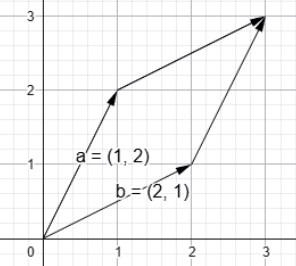
\includegraphics[scale=.5]{./tex/geo/pics/cross1.png}
\end{center}
la implementación también es sencilla y nos da una forma rápida de comprobar si tres puntos son colineales.
\lstinputlisting[language=C++]{./tex/geo/codes/cross.cpp}
Con lo anterior ya tenemos las herramientas suficientes para resolver nuestro problema de ordenar los puntos del plano de forma horaria o antihoraria alrededor de un punto.
\\
Supongamos que queremos ordenar los puntos del plano de forma antihoraria respecto al origen y con una referencia de ''inicio'' que tomaremos como $v=(0,1)$.
\\Notemos que si tenemos un conjunto de puntos $A$, podemos dividir el plano en dos partes, la primera que llamaremos $N$ que tendrá a todos los puntos que estén a la izquierda de $v$ y todos los puntos que sean colineales apuntando a la misma dirección, la segunda se llamará $S$ y serán los restantes, es decir, aquellos a la derecha de $v$ y los colineales que apuntan en dirección opuesta es decir, los puntos en el área roja estarían en $N$ y los del área azul en $S$.
\begin{center}
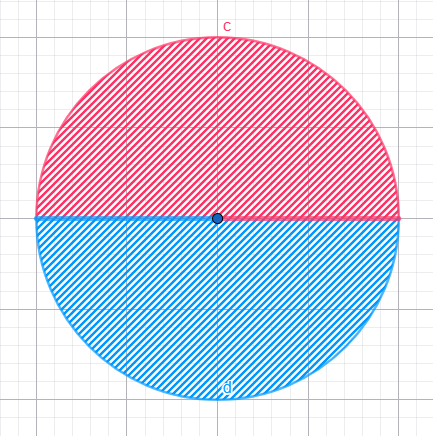
\includegraphics[scale=.5]{./tex/geo/pics/sort.png}
\end{center}
Entonces de aquí que digamos que para un punto $x$ en $A$, $x$ está en $N$ si y sólo si se cumple que $v\times x >0$ o $v\cdot x >0$ y además $v\times x=0$, estás siendo las operaciones de producto punto y cruz que vimos arriba, con esto podemos hacer una función que nos verifique si un punto de $A$ está o no en $N$ facilmente
\lstinputlisting[language=C++]{./tex/geo/codes/sort1.cpp}
Una vez dividido en dos partes notemos que dados $x$ y $y$, podemos decir que $x < y$ si $x \in N$ y $y \in S$ o ambos están en la misma parte y además $x \times y >0$, para esto entonces sólo nos basta definir un operador como sigue que es más fácil de manipular.
\lstinputlisting[language=C++]{./tex/geo/codes/sort2.cpp}



\chapter{Teoría de gráficas}
Una gráfica $G = (V, E)$ consiste en un conjunto de \textbf{vértices} $V$ y un conjunto de \textbf{aristas} $E \subseteq \binom{V}{2}$. Partimos de las nociones elementales de vecindad, grado, caminos, ciclos y conectividad, sin repetirlas aquí. Esta sección se enfoca en resultados matemáticos que fundamentan el resto del capítulo y que raramente se ven en cursos de computación.
\\\\
Existen dos representaciones estándar de una gráfica, con complejidades muy distintas:
\begin{itemize}
    \item \textbf{Lista de adyacencia}: conviene cuando el grafo es \emph{disperso}, es decir, cuando $E \ll V^2$.
    \item \textbf{Matriz de adyacencia}: conviene cuando se necesitan consultas de aristas en $O(1)$, o cuando $V$ es pequeño ($V \leq 500$) y ese costo de espacio es aceptable.
\end{itemize}
La tabla resume las operaciones más frecuentes en cada representación.

\begin{table}[H]
\centering
\renewcommand{\arraystretch}{1.4}
\begin{tabular}{lll}
\toprule
\textbf{Operación} & \textbf{Lista de adyacencia} & \textbf{Matriz de adyacencia} \\
\midrule
Espacio                    & $O(V + E)$  & $O(V^2)$ \\
¿Existe arista $(u,v)$?    & $O(\deg u)$ & $O(1)$ \\
Vecinos de $u$             & $O(\deg u)$ & $O(V)$ \\
Agregar arista             & $O(1)$      & $O(1)$ \\
\bottomrule
\end{tabular}
\end{table}
\section{Lema de los apretones de mano}
Si en una reunión cada persona estrecha la mano con algunos asistentes, podemos contar las ``manos involucradas'' de dos formas: sumando cuántas veces saludó cada persona, o bien contando cada apretón dos veces (una por cada extremo). El lema traduce esa idea a grafos: cada arista aporta $1$ al grado de cada uno de sus dos extremos.
\\\\
En todo grafo $G = (V, E)$:
\[
\sum_{v \in V} \deg(v) = 2|E|
\]

$Demostración$. Cada arista $\{u, v\}$ contribuye exactamente $1$ al grado de $u$ y $1$ al grado de $v$, es decir, contribuye $2$ a la suma total de grados. Sumando sobre todas las aristas: $\sum_v \deg(v) = 2|E|$. 

En todo grafo, el número de vértices de grado impar es par.
\\\\
$Demostración$.
Sea $I$ el conjunto de vértices de grado impar y $P$ el de grado par. Entonces:
\[
2|E| = \sum_{v \in I} \deg(v) + \sum_{v \in P} \deg(v)
\]
El segundo término es par (suma de números pares). Como $2|E|$ es par, el primer término también debe serlo.
\\\\
Este corolario tiene consecuencias sorprendentes en el ICPC. Por ejemplo: en un torneo (grafo dirigido completo), la suma de grados de salida es $\binom{n}{2}$; argumentos de paridad sobre los grados pueden determinar si cierta configuración es posible sin necesidad de construirla.

\section{Caminos y circuitos de Euler}
\subsection*{Los puentes de Königsberg}
En 1736, Leonhard Euler resolvió el siguiente problema planteado por los habitantes de la ciudad de Königsberg. La ciudad tenía 7 puentes que conectaban 4 zonas de tierra. ¿Es posible dar un paseo cruzando cada puente exactamente una vez y regresar al punto de partida?
\begin{figure}[H]
\centering
\begin{tikzpicture}[
  every node/.style={circle,draw,minimum size=0.8cm,font=\small},
  scale=1.2
]
  \node (A) at (0, 0)    {$A$};
  \node (B) at (3, 1.2)  {$B$};
  \node (C) at (3,-1.2)  {$C$};
  \node (D) at (6, 0)    {$D$};
 
  \draw (A) to[bend left=20]  node[draw=none,above,font=\scriptsize]{1}(B);
  \draw (A) to[bend right=20] node[draw=none,below,font=\scriptsize]{2}(B);
  \draw (A) to[bend left=20]  node[draw=none,above,font=\scriptsize]{3}(C);
  \draw (A) to[bend right=20] node[draw=none,below,font=\scriptsize]{4}(C);
  \draw (B) --                node[draw=none,right,font=\scriptsize]{5}(C);
  \draw (B) to[bend left=15]  node[draw=none,above,font=\scriptsize]{6}(D);
  \draw (C) to[bend right=15] node[draw=none,below,font=\scriptsize]{7}(D);
\end{tikzpicture}
\end{figure}
 
Euler demostró que tal paseo es \textbf{imposible} y al hacerlo fundó
la teoría de gráficas. Su argumento fue que cada vez que el paseo pasa por una
zona (sin empezar ni terminar ahí), usa un puente para entrar y otro
para salir. Por lo tanto esa zona debe tener un número par de puentes.
Las zonas $B$ y $C$ tienen 3 puentes cada una, así que el paseo
no puede existir.
 
\begin{definition}[Camino y circuito euleriano]
En una gráfica $G$:
\begin{itemize}
    \item Un \textbf{camino euleriano} es un camino que recorre cada
          arista exactamente una vez.
    \item Un \textbf{circuito euleriano} es un camino euleriano que
          empieza y termina en el mismo vértice.
    \item $G$ es \textbf{euleriano} si tiene un circuito euleriano.
\end{itemize}
\end{definition}
 
Sea $G$ conexa. Entonces:
\begin{itemize}
    \item $G$ tiene un \textbf{circuito euleriano} si y solo si todo
          vértice tiene grado par.
    \item $G$ tiene un \textbf{camino euleriano} (no circuito) si y solo
          si exactamente dos vértices tienen grado impar, y el camino
          debe empezar en uno de ellos y terminar en el otro.
\end{itemize}
\subsection{Algoritmo de Hierholzer}
 
Verificar si existe un circuito euleriano es fácil. Encontrarlo es lo que requiere el algoritmo de Hierholzer.
\\\\
Intuitivamente, el algoritmo parte de cualquier vértice y sigue aristas arbitrarias hasta regresar al punto de partida. Esto va a formar un circuito, pero puede no ser euleriano. Si algún vértice del circuito actual tiene aristas sin usar, se extiende el circuito
desde ese vértice. Se repite esto hasta usar todas las aristas.
 
\begin{lstlisting}[language=C++]
// Hierholzer: construye un circuito euleriano desde 'inicio'.
// Asume que adj[v] es la lista de vecinos (se consume al recorrer).
vector<int> hierholzer(int inicio) {
    stack<int> st;
    vector<int> circuito;
    st.push(inicio);

    while (!st.empty()) {
        int v = st.top();

        if (adj[v].empty()) {
            // No quedan aristas salientes: v entra al circuito.
            circuito.push_back(v);
            st.pop();
        } else {
            // Tomamos una arista v -> u y seguimos el recorrido.
            int u = adj[v].back();
            adj[v].pop_back();
            st.push(u);
        }
    }

    reverse(circuito.begin(), circuito.end());
    return circuito;
}
\end{lstlisting}
Muchos problemas se reducen a encontrar un camino o circuito euleriano
de forma no obvia. El patrón general es construir un grafo donde lo
que se quiere recorrer son las \textbf{aristas}, no los vértices. Imaginemos que nos dan
un conjunto de palabras y nos preguntan, ¿es posible ordenarlas en una secuencia tal que la última letra de cada palabra sea la primera de la siguiente? Podemos modelar cada letra como un vértice, cada palabra como una arista dirigida de su primera letra a su última. La
secuencia existe si y solo si el grafo tiene un camino euleriano.
\section{Componentes fuertemente conexas}
En un grafo \textbf{no dirigido}, la conectividad es simple, hay un
camino entre dos nodos o no. Pero en un grafo \textbf{dirigido} la
situación es más complicada, pues puede haber un camino de $u$ a $v$ sin que
haya uno de $v$ a $u$.
 
\begin{definition}
Una \textbf{componente fuertemente conexa} (SCC) de una gráfica dirigida
es un subconjunto maximo de vértices $C$ tal que para todo par
$u, v \in C$ existe un camino de $u$ a $v$ y un camino de $v$ a $u$.
\end{definition}
\subsection{Algoritmo de Kosaraju}
El algoritmo de Kosaraju encuentra todas las SCCs en $O(V + E)$ con dos DFS. Se apoya en el \textbf{grafo transpuesto} $G^T$ (mismos nodos, aristas invertidas). Las SCCs de $G$ y $G^T$ son las mismas, aunque cambia el orden en que conviene descubrirlas.
\\\\
El procedimiento tiene dos pasos:
\begin{enumerate}
    \item \textbf{DFS en $G$.} Al terminar de explorar cada nodo, lo añadimos al final de una lista \texttt{order}. Un nodo se registra tarde cuando aún quedaban descendientes por visitar; por eso el último de la lista pertenece a una SCC sin aristas entrantes desde otras componentes.
    \item \textbf{DFS en $G^T$, en orden inverso.} Recorremos \texttt{order} de atrás hacia adelante. Cada vez que encontramos un nodo sin componente asignada, lanzamos un DFS en $G^T$ desde ahí. Ese DFS descubre \emph{exactamente} una SCC: en $G^T$ las aristas que salían hacia otras componentes se volvieron entradas, así que no podemos salir de la componente actual.
\end{enumerate}
 
\begin{figure}[H]
\centering
\begin{tikzpicture}[
  every node/.style={circle,draw,minimum size=0.65cm,font=\small},
  scale=1.1
]
  \begin{scope}[->, >=stealth]
    \node (a) at (0,2)   {$a$};
    \node (b) at (2,3)   {$b$};
    \node (c) at (2,1)   {$c$};
    \node (d) at (4,2)   {$d$};
    \node (e) at (6,3)   {$e$};
    \node (f) at (6,1)   {$f$};
    \draw (a)--(b); \draw (b)--(c); \draw (c)--(a);
    \draw (b)--(d); \draw (c)--(d);
    \draw (d)--(e); \draw (e)--(f); \draw (f)--(d);
    \node[draw=none,font=\small] at (3,-0.3) {$G$};
  \end{scope}
 
  \begin{scope}[xshift=8cm, ->, >=stealth]
    \node (a2) at (0,2)  {$a$};
    \node (b2) at (2,3)  {$b$};
    \node (c2) at (2,1)  {$c$};
    \node (d2) at (4,2)  {$d$};
    \node (e2) at (6,3)  {$e$};
    \node (f2) at (6,1)  {$f$};
    \draw (b2)--(a2); \draw (c2)--(b2); \draw (a2)--(c2);
    \draw (d2)--(b2); \draw (d2)--(c2);
    \draw (e2)--(d2); \draw (f2)--(e2); \draw (d2)--(f2);
    \node[draw=none,font=\small] at (3,-0.3) {$G^T$};
  \end{scope}
\end{tikzpicture}
\end{figure}
 
En el ejemplo de la figura las SCCs son $\{a,b,c\}$ y $\{d,e,f\}$. Veamos el algoritmo paso a paso suponiendo que los nodos se numeran $a=0,b=1,c=2,d=3,e=4,f=5$ y que el primer DFS recorre $G$ en ese orden.

\textbf{Paso 1 (DFS en $G$).} Empezamos en $a$: visitamos $a \to b \to c$; desde $c$ seguimos a $d$, luego $d \to e \to f$, y al retroceder registramos cada nodo al terminar:
\[
\texttt{order} = [f,\, e,\, d,\, c,\, b,\, a].
\]
El último en la lista es $a$, de la componente $\{a,b,c\}$. Intuitivamente, al explorar desde $a$ ``empujamos'' todo el triángulo $\{d,e,f\}$ antes de cerrar $a$.

\textbf{Paso 2 (DFS en $G^T$, orden inverso).} Procesamos \texttt{order} de derecha a izquierda:
\begin{itemize}
    \item Desde $a$ (primero en este orden): en $G^T$ solo podemos retroceder por aristas invertidas dentro de $\{a,b,c\}$ (ciclo $a \to c \to b \to a$). Las flechas $b \to d$ y $c \to d$ de $G$ se vuelven $d \to b$ y $d \to c$ en $G^T$, pero $d$ aún no se visita desde $a$ porque esas aristas \emph{entran} a $\{a,b,c\}$, no salen de $a$. Resultado: $\{a,b,c\}$ recibe \texttt{comp} $= 0$.
    \item Los nodos $b$ y $c$ ya tienen componente; el siguiente libre es $d$. Desde $d$ en $G^T$ alcanzamos $e \to f \to d$ y también los predecesores $b,c$ (ya visitados). Solo se agrega $\{d,e,f\}$ con \texttt{comp} $= 1$.
\end{itemize}
Así cada llamada a \texttt{dfs2} aísla exactamente una SCC.
 
\begin{lstlisting}[language=C++]
vector<int> adj[MAXN], radj[MAXN];  // G y G^T
bool visited[MAXN];
vector<int> order;                  // orden de salida del primer DFS
int comp[MAXN];                     // SCC de cada nodo

void dfs1(int v) {
    visited[v] = true;
    for (int u : adj[v]) {
        if (!visited[u]) {
            dfs1(u);
        }
    }
    order.push_back(v);
}

void dfs2(int v, int c) {
    comp[v] = c;
    for (int u : radj[v]) {
        if (comp[u] == -1) {
            dfs2(u, c);
        }
    }
}

int kosaraju(int n) {
    // Primer DFS en G: construye el orden de salida.
    fill(visited, visited + n, false);
    for (int i = 0; i < n; i++) {
        if (!visited[i]) {
            dfs1(i);
        }
    }

    // Segundo DFS en G^T, en orden inverso de salida.
    fill(comp, comp + n, -1);
    int numScc = 0;
    for (int i = n - 1; i >= 0; i--) {
        int v = order[i];
        if (comp[v] == -1) {
            dfs2(v, numScc++);
        }
    }
    return numScc;
}
\end{lstlisting}
 
\subsection*{Gráfica de condensación}
 
Una vez encontradas las SCCs, podemos construir la \textbf{gráfica de
condensación}, una gráfica donde cada nodo representa una SCC y hay una arista de la SCC $i$ a la SCC $j$ si existe alguna arista en $G$ de un nodo en $i$ a un nodo en $j$. Esta gráfica siempre es un DAG (gráfica dirigida acíclica).
 
\begin{figure}[H]
\centering
\begin{tikzpicture}[
  every node/.style={circle,draw,minimum size=0.65cm,font=\small},
  scale=1.1, ->, >=stealth
]
  \begin{scope}
    \node (a) at (0,2)   {$a$};
    \node (b) at (2,3)   {$b$};
    \node (c) at (2,1)   {$c$};
    \node (d) at (4,2)   {$d$};
    \node (e) at (6,3)   {$e$};
    \node (f) at (6,1)   {$f$};
    \draw (a)--(b); \draw (b)--(c); \draw (c)--(a);
    \draw (b)--(d); \draw (c)--(d);
    \draw (d)--(e); \draw (e)--(f); \draw (f)--(d);
    \draw[teal,dashed,rounded corners] (-0.5,0.7) rectangle (2.6,3.8);
    \draw[red,dashed,rounded corners] (3.4,0.7) rectangle (6.7,3.8);
    \node[draw=none,teal,font=\scriptsize] at (1.0,4.2) {SCC 1};
    \node[draw=none,red,font=\scriptsize] at (5.0,4.2) {SCC 2};
  \end{scope}
 
  \begin{scope}[xshift=9cm]
    \node[fill=teal!20,minimum size=0.9cm]  (s1) at (0,2) {\scriptsize SCC1};
    \node[fill=red!20,minimum size=0.9cm] (s2) at (2,2) {\scriptsize SCC2};
    \draw (s1)--(s2);
    \node[draw=none,font=\small] at (1,0.8) {condensación (DAG)};
  \end{scope}
\end{tikzpicture}
\end{figure}
La gráfica de condensación es útil porque permite aplicar programación
dinámica sobre el DAG para resolver preguntas sobre la gráfica original.
\section{2-SAT\adv}
\advnote{Requiere componentes fuertemente conexas (sección anterior). Puede omitirse en una primera lectura.}
Motivemos esta sección con este problema: \href{https://codeforces.com/problemset/problem/776/D}{The door problem}. Se nos dice que hay $n$ personas atrapadas en $n$ cuartos (una puerta por cuarto). Hay $m$ interrumptores; en general $m$ puede ser mayor, igual o menor que $n$, y no hay relación fija entre ambos. Activar o desactivar un interrumptor cambia el estado de las puertas que controla. Cada puerta es controlada por exactamente dos interrumptores. ¿Es posible operar los
interruptores para que todas las puertas queden desbloqueadas al mismo
tiempo?
\\\\
Para resolver este problema, usaremos componentes fuertemente conexas, en este momento puede que el lector no vea la relación entre las $SCC$ y el problema, pero esta sección buscará reducir el problema a $SCC$.
\\\\
Supongamos que tenemos $n$ variables booleanas, cada una puede ser verdadera ($V$) o falsa ($F$). Las \textbf{restricciones} exigen que ciertas condiciones se cumplan; cada una involucra dos literales (una variable o su negación) unidos por ``o''. Por ejemplo, con $n = 3$:
\begin{itemize}
    \item $(x_1 \lor x_2)$: al menos uno de $x_1$, $x_2$ debe ser verdadero.
    \item $(\neg x_1 \lor x_3)$: si $x_1$ es falso, entonces $x_3$ debe ser verdadero.
    \item $(\neg x_2 \lor \neg x_3)$: $x_2$ y $x_3$ no pueden ser verdaderos a la vez.
\end{itemize}
La asignación $x_1 = V,\; x_2 = F,\; x_3 = V$ satisface las tres. En general, la pregunta es: ¿existe una asignación de verdadero/falso a \emph{todas} las variables que cumpla \emph{todas} las restricciones?
\\\\
A diferencia del problema general de satisfacibilidad (que es
NP-completo), cuando cada restricción involucra \textbf{exactamente
dos variables} el problema se puede resolver en $O(V + E)$ usando SCCs.
Este caso especial se llama \textbf{2-SAT}.
\\\\
La observación fundamental que reduce este problema a $SCC$ es que toda disyunción de 2 literales $(a \lor b)$ es equivalente a dos implicaciones:
\[
\neg a \Rightarrow b \qquad \text{y} \qquad \neg b \Rightarrow a
\]
Si $a$ es falso, entonces $b$ debe ser verdadero (y viceversa).
\\\\
Esto permite construir una gráfica dirigida con $2n$ nodos ($x_i$ y $\neg x_i$ para cada variable) donde cada disyunción agrega dos aristas.
 
\begin{figure}[H]
\centering
\begin{tikzpicture}[
  every node/.style={circle,draw,minimum size=0.75cm,font=\small},
  scale=1.1, ->, >=stealth
]
  \node (x1)  at (0,3)   {$x_1$};
  \node (nx1) at (0,1.5) {$\neg x_1$};
  \node (x2)  at (3,3)   {$x_2$};
  \node (nx2) at (3,1.5) {$\neg x_2$};
  \node (x3)  at (6,3)   {$x_3$};
  \node (nx3) at (6,1.5) {$\neg x_3$};
 
  \draw[teal] (nx1)--node[draw=none,below,font=\scriptsize]{$\neg x_1\Rightarrow x_2$}(x2);
  \draw[teal] (nx2)--node[draw=none,above,font=\scriptsize]{$\neg x_2\Rightarrow x_1$}(x1);
 
  \draw[red] (x2)--node[draw=none,above,font=\scriptsize]{$x_2\Rightarrow x_3$}(x3);
  \draw[red] (nx3)--node[draw=none,above,font=\scriptsize]{$\neg x_3\Rightarrow\neg x_2$}(nx2);
 
  \node[draw=none,font=\scriptsize,teal]  at (1.5,0.6) {$(x_1\lor x_2)$};
  \node[draw=none,font=\scriptsize,red] at (4.5,0.6) {$(\neg x_2\lor x_3)$};
\end{tikzpicture}
\end{figure}

Una fórmula 2-SAT es satisfacible si y solo si en el grafo de implicaciones ninguna variable $x_i$ está en la misma SCC que su negación $\neg x_i$. Si la fórmula es satisfacible, la asignación se obtiene directamente de los números de SCC que asigna Kosaraju:
 
\begin{itemize}
    \item $x_i = \text{verdadero}$ si $\text{comp}(x_i) > \text{comp}(\neg x_i)$
    \item $x_i = \text{falso}$ si $\text{comp}(x_i) < \text{comp}(\neg x_i)$
\end{itemize}
Kosaraju numera las SCCs de forma que si existe una implicación de la SCC $A$ hacia la SCC $B$, entonces $A$ recibe un número menor que $B$. La SCC con número mayor es la ``consecuencia'' de la cadena de implicaciones. Asignar verdadero a la variable cuya
SCC tiene número mayor garantiza que ninguna implicación se viola, siempre se va de falso hacia verdadero, nunca al revés.
\\\\
\\\\
En el problema de las puertas, cada puerta controlada por los interruptores $a$ y $b$ genera restricciones de exactamente esta forma.
\\\\Si la puerta está abierta, necesitamos que ambos interrumptores que la controlan se activen (sean verdaderos) o que ninguno lo haga (sean falsos). 
Esto se expresa con dos restricciones:
\begin{itemize}
    \item Si $x_a$ es verdadero, $x_b$ también debe serlo:
          $(\neg x_a \lor x_b)$
    \item Si $x_b$ es verdadero, $x_a$ también debe serlo:
          $(x_a \lor \neg x_b)$
\end{itemize}
Si está bloqueada, necesitamos que solamente uno de los interrumptores se active.
\begin{itemize}
    \item Si $x_a$ es verdadero, $x_b$ debe ser falso:
          $(\neg x_a \lor \neg x_b)$
    \item Si $x_a$ es falso, $x_b$ debe ser verdadero:
          $(x_a \lor x_b)$
\end{itemize}
Para resolver el problema entonces basta con construir la gráfica, correr Kosaraju y verificar que ningún $x_i$ esté en la misma SCC que $\neg x_i$.

\textbf{Ejercicio.} Implementar la solución del problema \href{https://codeforces.com/problemset/problem/776/D}{The door problem}.
 
\section{Puentes y puntos de articulación}
Para esta sección, pensemos el siguiente problema llamado \href{https://onlinejudge.org/external/3/315.pdfL}{Network}. En este problema, nos dicen que hay $n$ centrales de telefonía conectadas por cables bidireccionales de forma que desde cualquier central se puede llegar a otra no necesariamente de forma directa. En ocasiones, puede haber un apagón en alguna central por lo que deja de operar. Esto puede causar que otras centrales queden incomunicadas entre sí, en tal caso se dice son centrales críticas. Nos piden encontrar cuántas centrales son críticas.
\\\\
Nótese el siguiente ejemplo, si la central $4$ falla, las centrales
  $\{5,6\}$ quedan incomunicadas de $\{1,2,3\}$.
 
\begin{figure}[H]
\centering
\begin{tikzpicture}[
  every node/.style={circle,draw,minimum size=0.65cm,font=\small},
  scale=1.1
]
  \node (1) at (0,1.5)  {1};
  \node (2) at (1.5,3)  {2};
  \node (3) at (1.5,0)  {3};
  \node[fill=orange!20] (4) at (3,1.5) {4};
  \node (5) at (4.5,3)  {5};
  \node (6) at (4.5,0)  {6};
 
  \draw (1)--(2) (2)--(3) (3)--(1);
  \draw (2)--(4) (3)--(4);
  \draw (4)--(5) (4)--(6) (5)--(6);
 
  \node[draw=none,font=\scriptsize,orange!80!black] at (3,0.7)
    {crítica};
\end{tikzpicture}
\end{figure}
  
\begin{definition}[Puente y punto de articulación]
En un grafo conexo $G$:
\begin{itemize}
    \item Una arista es un \textbf{puente} si al eliminarla el grafo
          se desconecta.
    \item Un vértice es un \textbf{punto de articulación} si al
          eliminarlo (junto con sus aristas incidentes) el grafo se
          desconecta.
\end{itemize}
\end{definition}

En la siguiente gráfica, la arista roja $d$-$e$ es un puente. Los vértices $d$ y $e$ porque al eliminarlos desconectan la gráfica.
\begin{figure}[H]
\centering
\begin{tikzpicture}[
  every node/.style={circle,draw,minimum size=0.65cm,font=\small},
  scale=1.1
]
  \node (a) at (0,1.5)  {$a$};
  \node (b) at (1.5,3)  {$b$};
  \node (c) at (1.5,0)  {$c$};
  \node[fill=orange!20] (d) at (3,1.5)  {$d$};
  \node[fill=orange!20] (e) at (4.5,3)  {$e$};
  \node (f) at (6,1.5)  {$f$};
  \node (g) at (4.5,0)  {$g$};
 
  \draw (a)--(b) (b)--(c) (c)--(a);
  \draw (b)--(d) (c)--(d);
  \draw[red,very thick] (d)--(e);
  \draw (e)--(f) (f)--(g) (g)--(e);
 
  \node[draw=none,font=\scriptsize,red]            at (3.5,2.8) {puente};
  \node[draw=none,font=\scriptsize,orange!80!black] at (3,0.7)  {articulación};
  \node[draw=none,font=\scriptsize,orange!80!black] at (5.8,3)  {articulación};
\end{tikzpicture}
\end{figure}
Regresando al problema de las centrales, notemos que el problema nos pide imprimir cuántos puntos de articulación tiene la gráfica dada. Podríamos intentar revisar cada vértice y ver si al quitarlo desconecta la gráfica con $BFS/DFS$ pero esto costaría $O((V+E)V)$ lo que nos daría $TLE$, necesitamos algo más eficiente.
\\\\
Al hacer DFS, el árbol de llamadas forma un árbol DFS. Las
aristas que no forman parte de este árbol conectan un nodo con algún \textbf{ancestro} suyo les llamaremos aristas hacia atrás.
\\\\
La idea para cosntruir un algoritmo más eficiente es ver que un nodo $U$ es punto de articulación si tiene algún hijo $V$ tal que
\textbf{ningún nodo del subárbol de $V$ puede llegar a un ancestro de
$U$ sin pasar por $U$}. Para revisar esto, asignamos a cada vértice
un tiempo de descubrimiento $\texttt{disc}[v]$ que corresponde al orden
en que el DFS lo visitó. Ahora definimos $\texttt{low}[v]$ como el menor $\texttt{disc}$ alcanzable desde el subárbol de $v$:
\[
\texttt{low}[v] = \min \begin{cases}
\texttt{disc}[v] \\
\texttt{disc}[u] & \text{para toda arista hacia atrás } (v,u) \\
\texttt{low}[w] & \text{para todo hijo } w \text{ de } v \text{ en el árbol DFS}
\end{cases}
\]
Intuitivamente, $\texttt{low}[v]$ mide qué tan ``arriba'' puede
escapar el subárbol de $v$ sin usar la arista que lo conecta a su padre. En la siguiente gráfica $v$ tiene $low=0$ porque tiene una arista hacia atrás que le permite llegar a $r$ que tiene $low=0$ sin pasar por su padre. De forma similar, $u$ hereda el $low=0$ de su hijo $u$.
 
\begin{figure}[H]
\centering
\begin{tikzpicture}[
  every node/.style={circle,draw,minimum size=0.65cm,font=\small},
  scale=1.1, ->, >=stealth
]
  \node (r) at (3,4)   {$r$};
  \node (u) at (3,2.5) {$u$};
  \node (v) at (3,1)   {$v$};
  \node (w) at (1.5,1) {$w$};
 
  \draw (r)--(u) (u)--(v) (u)--(w);
  \draw[teal,dashed,->] (v) to[bend right=50]
    node[draw=none,right,font=\scriptsize,teal]{arista hacia atrás}(r);
 
  \node[draw=none,left,font=\scriptsize] at (2.5,4.0)
    {$\texttt{disc}[r]=0,\ \texttt{low}[r]=0$};
  \node[draw=none,left,font=\scriptsize] at (2.5,2.5)
    {$\texttt{disc}[u]=1,\ \texttt{low}[r]=0$};
  \node[draw=none,right,font=\scriptsize] at (3.4,1)
    {$\texttt{disc}[v]=2,\ \texttt{low}[v]=0$};
  \node[draw=none,left,font=\scriptsize]  at (1.1,1)
    {$\texttt{disc}[w]=3,\ \texttt{low}[w]=3$};
\end{tikzpicture}
\end{figure}
Para que una arista $(uv)$  con $v$ hijo de $u$ n el DFS sea un puente, se debe cumplir que $\texttt{low}[v] > \texttt{disc}[u]$. Ya que eso significa que el subárbol de $v$ no puede alcanzar a $u$ sin pasar por la arista $(u,v)$. Dicho esto, es lógico que la condición para que un vértice $u$ sea punto de articulación sea:
\begin{itemize}
    \item Si $u$ es la raíz del DFS, es punto de articulación si tiene
          $\geq 2$ hijos en el árbol DFS.
    \item Si $u$ no es raíz, es punto de articulación si tiene algún hijo $v$ tal con $\texttt{low}[v] \geq \texttt{disc}[u]$.
\end{itemize}
Finalmente, la implementación nos quedaría:
\begin{lstlisting}[language=C++]
vector<int> adj[MAXN];
int disc[MAXN], low[MAXN], timer = 0;
bool visited[MAXN], art[MAXN];
vector<pair<int, int>> bridges;

void dfs(int u, int parent) {
    visited[u] = true;
    disc[u] = low[u] = timer++;
    int children = 0;

    for (int v : adj[u]) {
        if (!visited[v]) {
            children++;
            dfs(v, u);
            low[u] = min(low[u], low[v]);

            // Arista u-v es puente.
            if (low[v] > disc[u]) {
                bridges.push_back({u, v});
            }

            // u es articulacion (caso no raiz).
            if (parent != -1 && low[v] >= disc[u]) {
                art[u] = true;
            }
        } else if (v != parent) {
            // Arista hacia atras.
            low[u] = min(low[u], disc[v]);
        }
    }

    // u es articulacion (caso raiz).
    if (parent == -1 && children >= 2) {
        art[u] = true;
    }
}
\end{lstlisting}
\textbf{Ejercicio.} Implementar la solución completa de \href{https://onlinejudge.org/external/3/315.pdfL}{Network} usando
este algoritmo.
 
\section{Árboles}
 
Un \textbf{árbol} es un grafo conexo, es decir, todos sus vértices están conectados por un camino, sin ciclos. Esta definición es solo una de varias caracterizaciones equivalentes, todas igualmente válidas como definición y útiles en distintos contextos.
 
Para un grafo $G$ con $n$ vértices, las siguientes afirmaciones son equivalentes:
\begin{enumerate}
    \item $G$ es conexo y acíclico.
    \item $G$ es conexo y tiene exactamente $n-1$ aristas.
    \item Entre todo par de vértices existe exactamente un camino simple.
\end{enumerate}
 
La caracterización (3), camino único entre todo par, será importante porque convierte preguntas sobre caminos en preguntas sobre estructura del árbol. Es la base del LCA y de la mayoría de técnicas sobre árboles.
 
Para motivar este capítulo de árboles, véamos el problema \href{https://codeforces.com/contest/342/problem/E}{Xenia and Tree}, en este nos dan un árbol con n nodos. El nodo $1$ está pintado de rojo y los demás de azul. Nos darán queries de dos tipos:
\begin{itemize}
    \item[1.] Nos dan un numero $a$ que corresponde a un nodo azul y tenemos que pintarlo rojo.
    \item[2.] Nos dan un numero $b$ que corresponde a un nodo del arbol y tenemos que imprimir la distancia entre $b$ y el nodo rojo más cercano.
\end{itemize}
Nótese que calcular la distancia a cada uno de los nodos rojos cada que nos dan una querie no es eficiente y en este problema que nos pueden dar $10^5$ queries en un arbol de $10^5$ vértices, esta solución ingenua resultaría en $TLE$. Veremos algunas herramientas que nos ayudarían a resolver este problema.

\section{Centroide\adv}
\advnote{Requiere manejo cómodo de árboles (DFS, subtamaños). Puede omitirse en una primera lectura.}
 
El \textbf{centroide} de un árbol es un vértice $c$ tal que al eliminarlo, ninguna componente conexa resultante tiene más de $\lfloor n/2 \rfloor$ vértices. Todo árbol tiene uno o dos centroides. Si tiene dos, son adyacentes. En la siguiente figura el vértice amarillo es el centroide, nótese que entonces si se elimina las componentes conexas se quedan con un vértice.
 
\begin{figure}[H]
\centering
\begin{tikzpicture}[
  every node/.style={circle, draw, minimum size=0.65cm, font=\small},
  scale=1.0
]
  \node[fill=yellow!40] (c) at (3, 2) {$c$};
  \node (a) at (1, 3)   {$a$};
  \node (b) at (1, 2)   {$b$};
  \node (d) at (1, 1)   {$d$};
  \node (e) at (5, 3)   {$e$};
  \node (f) at (5, 2)   {$f$};
  \node (g) at (4, 1)   {$g$};
  \node (h) at (6, 1)   {$h$};
  \node (i) at (3, 0.5) {$i$};
 
  \draw (c)--(a) (c)--(b) (c)--(d) (c)--(e) (c)--(f) (c)--(g) (c)--(h) (c)--(i);
\end{tikzpicture}
\end{figure}
 
\subsubsection*{Descomposición por centroide}

Tomemos un árbol más grande que el anterior y tomemos su centroide $c$. Al eliminarlo, el árbol se divide en varias componentes, cada una de tamaño $\leq \lfloor n/2 \rfloor$. Nótese que entonces cualquier camino de un nodo $v$ en una componente a otro $u$ en otra componente, este pasa por $c$, entonces si quisieramos la distancia entre $u$ y $v$ podemos sumar la distancia entre $c$ y $v$ y la distancia entre $c$ y $u$.

\begin{figure}[H]
\centering
\begin{tikzpicture}[
  every node/.style={circle, draw, minimum size=0.65cm, font=\small},
  scale=1.0
]
  \node[fill=yellow!40] (c) at (4, 3) {$c$};
 
  \node (a) at (1.5, 4.5) {$a$};
  \node (b) at (1.5, 3.0) {$b$};
  \node (e) at (0.0, 3.0) {$e$};
 
  \node (f) at (4.0, 1.5) {$f$};
  \node (g) at (3.0, 0.5) {$g$};
 
  \node (h) at (6.5, 4.5) {$h$};
  \node (i) at (6.5, 3.0) {$i$};
  \node (j) at (8.0, 3.0) {$j$};
 
  \draw (b)--(a) (c)--(b) (c)--(f) (c)--(h);
 
  \draw (b)--(e) (f)--(g) (h)--(i) (i)--(j);
 
  \draw[dashed, teal, rounded corners] (-0.5,2.5) rectangle (2.2,5.2);
  \draw[dashed, red, rounded corners] (2.5,0.0) rectangle (4.8,2.2);
  \draw[dashed, blue!40, rounded corners] (5.8,2.5) rectangle (8.7,5.2);
 
  \node[draw=none, teal, font=\scriptsize] at (0.85, 5.5) {comp. 1};
  \node[draw=none, red, font=\scriptsize] at (3.65, -0.4) {comp. 2};
  \node[draw=none, blue!40, font=\scriptsize] at (7.25, 5.5) {comp. 3};
\end{tikzpicture}
\end{figure}
 La observación anterior solo resuelve caminos entre componentes distintas. Pero los nodos rojos también pueden estar en la misma componente que $v$. La solución es aplicar el mismo argumento recursivamente, cada componente tiene su propio centroide, y todo camino dentro de ella que no pasa por ese centroide, pasará por el centroide de alguna subcomponente más pequeña.

 Esto define el \textbf{árbol de centroide}: tomamos el centroide $c$ del árbol completo como raíz, recursamos en cada componente que queda al eliminarlo, y los centroides de esas componentes se vuelven hijos de $c$ en el árbol de centroide.
 
\begin{figure}[H]
\centering
\begin{tikzpicture}[
  every node/.style={circle, draw, minimum size=0.65cm, font=\small},
  scale=1.0
]
  \node[fill=yellow!40] (c)  at (4.0, 4.0) {$c$};
  \node[fill=yellow!20] (c1) at (1.5, 2.5) {$b$};
  \node[fill=yellow!20] (c2) at (4.0, 2.5) {$f$};
  \node[fill=yellow!20] (c3) at (6.5, 2.5) {$i$};
  \node (e)  at (0.5, 1.0) {$e$};
  \node (a)  at (2.5, 1.0) {$a$};
  \node (g)  at (4.0, 1.0) {$g$};
  \node (h)  at (5.5, 1.0) {$h$};
  \node (j)  at (7.5, 1.0) {$j$};
 
  \draw (c)--(c1) (c)--(c2) (c)--(c3);
  \draw (c1)--(e) (c1)--(a);
  \draw (c2)--(g);
  \draw (c3)--(h) (c3)--(j);
 
  \node[draw=none, font=\small, gray] at (-0.8, 4.0) {nivel 0};
  \node[draw=none, font=\small, gray] at (-0.8, 2.5) {nivel 1};
  \node[draw=none, font=\small, gray] at (-0.8, 1.0) {nivel 2};
\end{tikzpicture}
\end{figure}

Notemos entonces que para cualquier par de nodos $u$ y $v$, existe un ancestro común en el árbol de centroide tal que el camino entre los nodos en el árbol original pasa por ese ancestro, el cual es el ancestro común de $u$ y $v$, por ejemplo, para $g$ y $e$ en el árbol anterior, este es $c$, es decir el primer ancestro que comparten. En caso de $e$ y $a$, es $b$.

%NOTA (buscar algun recuadro de color para estas cosas)
Una propiedad importante es que el árbol de centroide tiene profundidad $O(\log n)$, ya que cada vez que bajamos un nivel, el subárbol tiene tamaño $\leq \lfloor n/2 \rfloor$ (por la propiedad del centroide). Tras $k$ niveles el tamaño es $\leq n/2^k$. La recursión termina cuando el tamaño llega a 1, es decir a profundidad $\lceil \log_2 n \rceil$, esto es relevante para calcular la compleljidad del algortimo.

Volviendo al problema, con el árbol de centroide construido, mantenemos para cada nodo $c$:
\[
\texttt{minDist}[c] = \min_{u \text{ rojo}} \text{dist}(c,\, u)
\]
la distancia mínima desde $c$ a cualquier nodo rojo en el subárbol \emph{original} sobre el que $c$ fue centroide. Inicialmente $\texttt{minDist}[c] = \infty$ para todo $c$. Ahora, cada que recibamos una query del tipo $1$, en la que nos pidan pintar un vértice $v$ de rojo, para todo nodo $c$ ancestro de $v$ en el árbol de centroide, debemos actualizar:
\[
\texttt{minDist}[c] \leftarrow \min\, \!\bigl(\texttt{mindist}[c],\ \text{dist}(v, c)\bigr)
\]
Como hay $O(\log n)$ ancestros, esta operación cuesta $O(\log n)$ llamadas a \texttt{dist}.
 
\medskip
Para el segundo tipo de query notemos que para cualquier nodo rojo $u$, existe un ancestro $c$ de $v$ en el árbol de centroide tal que el camino de $v$ a $u$ pasa por $c$.
Entonces la respuesta es:
\[
\min_{c \text{ ancestro de } v \text{ en árbol de centroide}} \bigl(\text{dist}(v, c) + \texttt{minDist}[c]\bigr)
\]
De nuevo $O(\log n)$ llamadas a \texttt{dist}.
\\\\
Podría parecer que ya logramos optimizar la solución, sin embargo, estamos olvidando un detalle ¿cuánto cuesta calcular $\text{dist}(v, c)$?
\\\\
La forma más directa es hacer un BFS o DFS desde $c$ cada vez, pero eso cuesta $O(n)$ por llamada. Con $O(\log n)$ ancestros por query y $m$ queries, el costo total sería $O(mn \log n)$ que para $n = m = 10^5$ da $\sim 10^{11}$ operaciones. Demasiado lento.
\\\\
Necesitamos calcular $\text{dist}(u, v)$ en $O(\log n)$. Esto se logra con el \textbf{ancestro común más bajo} (LCA), que veremos en la siguiente sección.
\\\\
La implementación para construir el árbol de centroide queda:
\begin{lstlisting}[language=C++]
const int MAXN = 100005;

vector<int> g[MAXN];   // grafica original
int sz[MAXN];          // tamano del subarbol en la componente actual
bool removed[MAXN];    // true si el nodo ya fue usado como centroide
int cpar[MAXN];        // padre en el arbol de centroide (-1 para la raiz)

// Calcula el tamano del subarbol de u en la componente actual.
int calcSz(int u, int p) {
    sz[u] = 1;
    for (int v : g[u]) {
        if (v != p && !removed[v]) {
            sz[u] += calcSz(v, u);
        }
    }
    return sz[u];
}

// Encuentra el centroide de la componente que contiene a u.
int centroid(int u, int p, int treeSz) {
    for (int v : g[u]) {
        if (v != p && !removed[v] && sz[v] > treeSz / 2) {
            return centroid(v, u, treeSz);
        }
    }
    return u;
}

// Construye el arbol de centroide recursivamente.
// u: cualquier nodo de la componente actual.
// p: padre en el arbol de centroide (-1 para la raiz).
void build(int u, int p) {
    int total = calcSz(u, -1);
    int c = centroid(u, -1, total);

    cpar[c] = p;
    removed[c] = true;

    // Recursar en cada componente que queda al eliminar c.
    for (int v : g[c]) {
        if (!removed[v]) {
            build(v, c);
        }
    }
}
\end{lstlisting}
 El patrón estándar para cualquier problema que use descomposición por centroide es este problema, subir por los $O(\log n)$ ancestros en el árbol de centroide y agregar o consultar información en cada uno. Lo que varía entre problemas es qué información se guarda y cómo se combina.
\section{Ancestro común más bajo (LCA)\adv}
\advnote{Requiere árboles con raíz y, para la versión eficiente, preprocesamiento (binary lifting). Puede omitirse en una primera lectura.}
Dado un árbol con raíz, el \textbf{ancestro común más bajo} (LCA) de dos vértices $u$ y $v$ es el vértice más abajo que es ancestro de ambos.
\begin{figure}[H]
\centering
\begin{tikzpicture}[
  every node/.style={circle, draw, minimum size=0.65cm, font=\small},
  scale=1.1
]
  \node (r) at (4, 4)   {$r$};
  \node (a) at (2, 3)   {$a$};
  \node (b) at (6, 3)   {$b$};
  \node (c) at (1, 2)   {$c$};
  \node[fill=yellow!40] (d) at (3, 2) {$d$};
  \node (e) at (5, 2)   {$e$};
  \node (f) at (7, 2)   {$f$};
  \node[fill=teal!20] (u) at (2, 1)   {$u$};
  \node[fill=teal!20] (v) at (4, 1)   {$v$};
 
  \draw (r)--(a) (r)--(b) (a)--(c) (a)--(d) (b)--(e) (b)--(f) (d)--(u) (d)--(v);
 
  \draw[teal!60, very thick, dashed] (u)--(d)--(v);
  \node[draw=none, font=\scriptsize, teal] at (3, 0.5) {$\text{LCA}(u,v) = d$};
\end{tikzpicture}
\end{figure}
La solución más directa que podríamos pensar es ver qué nodo está más bajo o profundo y llevarlo al mismo nivel que el otro subiendo de a un paso, luego subir ambos juntos hasta que coincidan. Por ejemplo para $c$ y $u$ en la figura de arriba, primero subiríamos $u$ a su ancestro $d$ y ya que ambos $d$ y $c$ estpan en el mismo nivel, los subiriamos a su ancestro $a$ que como coincide, diríamos que este es su $LCA$.
\\\\
Imaginemos que tenemos un árbol en forma de cadena ($1 - 2 - 3 - \cdots - n$), calcular $\text{LCA}(1, n)$ cuesta $O(n)$ pasos. Con $m$ queries, el costo total es $O(mn)$, lo que nos deja con el mismo problema que teníamos antes, necesitamos algo más eficiente. En lugar de subir de $1$ en $1$, ¿podríamos subir de a $2^k$ niveles de una vez?
\\\\
 Para subir $d$ niveles desde un nodo $v$, podemos descomponer $d$ en potencias de 2 (como en la representación binaria) y dar saltos de tamaño $1, 2, 4, 8, \ldots$ según corresponda. Si $d = 13 = 8 + 4 + 1$, damos un salto de 8, luego uno de 4, luego uno de 1, tres saltos en lugar de 13.
\\\\
Entonces necesitamos precalcular, para cada nodo $v$ y cada $k$:
\[
\texttt{up}[v][k] = \text{ancestro de } v \text{ a distancia } 2^k
\]
La forma de calcular esto será con una recurrencia, el ancestro a distancia $2^k$ es el ancestro a distancia $2^{k-1}$ del ancestro a distancia $2^{k-1}$:
\[
\texttt{up}[v][0] = \text{padre}(v), \qquad \texttt{up}[v][k] = \texttt{up}[\texttt{up}[v][k-1]][k-1]
\]
 
Como estamos subiendo en potencias de $2$, $\lfloor \log_2 n \rfloor + 1$ niveles basta para cubrir cualquier distancia hasta $n$. En la siguiente imagen, vemos como para el arbol que es una cadena que mencionamos antes, esta forma de encontrar el ancestro sí resulta eficiente. Para el nodo $v$, los ancestros a distancia $2^0=1$, $2^1=2$ y $2^2=4$ se precalculan. Para subir 5 niveles, basta un salto de 4 y un salto de 1, solo 2 operaciones.
 
\begin{figure}[H]
\centering
\begin{tikzpicture}[
  every node/.style={circle, draw, minimum size=0.65cm, font=\small},
  scale=1.0
]
  \node (r)  at (4.0, 5.0) {$r$};
  \node (a)  at (4.0, 4.0) {$a$};
  \node (b)  at (4.0, 3.0) {$b$};
  \node (c)  at (4.0, 2.0) {$c$};
  \node (d)  at (4.0, 1.0) {$d$};
  \node[fill=teal!20] (v)  at (4.0, 0.0) {$v$};
 
  \draw (r)--(a)--(b)--(c)--(d)--(v);
 
  \draw[teal, thick, ->] (v.west) to[bend left=40]
    node[draw=none, left, font=\scriptsize] {$2^0=1$} (d.west);
 
  \draw[orange, thick, ->] (v.east) to[bend right=50]
    node[draw=none, right, font=\scriptsize] {$2^1=2$} (c.east);
 
  \draw[red, thick, ->] (v.east) to[bend right=70]
    node[draw=none, right=0.6cm, font=\scriptsize] {$2^2=4$} (a.east);
\end{tikzpicture}
\end{figure}

Lo que haremos entonces para calcular el $LCA$  de dos nodos $u$ y $v$ será primero igualar sus profundidades. Si $\text{prof}(u) > \text{prof}(v)$, necesitamos subir $u$ exactamente $d = \text{prof}(u) - \text{prof}(v)$ niveles. Descomponemos $d$ en binario y usamos los saltos correspondientes.
\\\\
Una vez que coinciden, revisamos si $u = v$, ai se cumple, ese es el LCA. De lo contrario, subimos ambos nodos simultáneamente, usando el salto más grande posible tal que $\texttt{up}[u][k] \neq \texttt{up}[v][k]$ (es decir, que no hayan convergido todavía). Después de este proceso, $u$ y $v$ son hijos del LCA.

\begin{lstlisting}[language=C++]
const int LOG = 17;
int up[MAXN][LOG];  // up[v][k] = ancestro de v a distancia 2^k
int prof[MAXN];

// Precalcula ancestros con DFS desde la raiz.
void dfs(int v, int p, int d) {
    up[v][0] = p;
    prof[v] = d;

    for (int k = 1; k < LOG; k++) {
        up[v][k] = up[up[v][k - 1]][k - 1];
    }

    for (int u : g[v]) {
        if (u != p) {
            dfs(u, v, d + 1);
        }
    }
}

int lca(int u, int v) {
    // Igualar profundidades.
    if (prof[u] < prof[v]) {
        swap(u, v);
    }
    int diff = prof[u] - prof[v];
    for (int k = 0; k < LOG; k++) {
        if ((diff >> k) & 1) {
            u = up[u][k];
        }
    }

    if (u == v) {
        return u;
    }

    // Subir ambos nodos juntos hasta quedar justo debajo del LCA.
    for (int k = LOG - 1; k >= 0; k--) {
        if (up[u][k] != up[v][k]) {
            u = up[u][k];
            v = up[v][k];
        }
    }

    return up[u][0];
}
\end{lstlisting}

Notemos que para calcular la distancia entre dos nodos $u$ y $v$, el camino de $u$ a $v$ sube desde $u$ hasta el LCA $d$ y luego baja hasta $v$. La distancia total es la suma de los dos tramos, que se simplifica a $\text{prof}(u)+\text{prof}(v)-2\cdot\text{prof}(\text{LCA})$.
\begin{figure}[H]
\centering
\begin{tikzpicture}[
  every node/.style={circle, draw, minimum size=0.7cm, font=\small},
  scale=1.15
]
 
\node (r) at (4.0, 5.0) {$r$};
\node (a) at (2.0, 4.0) {$a$};
\node (b) at (6.0, 4.0) {$b$};
\node (c) at (1.0, 3.0) {$c$};
\node[fill=yellow!40] (d) at (3.0, 3.0) {$d$};
\node (e) at (5.0, 3.0) {$e$};
\node (f) at (7.0, 3.0) {$f$};
\node[fill=teal!20] (u) at (2.0, 2.0) {$u$};
\node[fill=teal!20] (v) at (4.0, 2.0) {$v$};
 
\draw[gray!60] (r)--(a) (r)--(b);
\draw[gray!60] (a)--(c) (a)--(d);
\draw[gray!60] (b)--(e) (b)--(f);
 
\draw[teal, very thick] (u)--(d)--(v);
 
\draw[dashed, gray!50] (3.0, 4.85) -- (3.0, 3.35);
\draw[gray!50] (3.0, 4.85) -- (3.2, 4.85);
\draw[gray!50] (3.0, 3.35) -- (3.2, 3.35);
\node[draw=none, right, font=\scriptsize, text=gray] at (3.2, 4.1) {$\text{prof}(d) = 2$};
 
\draw[teal!60, dashed] (0.5, 4.85) -- (0.5, 2.35);
\draw[teal!60] (0.5, 4.85) -- (0.7, 4.85);
\draw[teal!60] (0.5, 2.35) -- (0.7, 2.35);
\node[draw=none, left, font=\scriptsize, text=teal!80!black] at (0.5, 3.6)
  {$\text{prof}(u) = 3$};
 
\node[draw=none, below right, font=\scriptsize, text=orange!70!black] at (2.5, 4.1)
  {\textbf{LCA}$(u,v)$};
 
\node[draw=none, right, font=\small] at (7.8, 3.5) {
  $\begin{aligned}
    \text{dist}(u,v)
      &= \underbrace{\text{prof}(u) - \text{prof}(d)}_{\text{subida}} 
       + \underbrace{\text{prof}(v) - \text{prof}(d)}_{\text{bajada}}\\[4pt]
      &= \text{prof}(u) + \text{prof}(v) - 2\cdot\text{prof}(d)\\[4pt]
      &= 3 + 3 - 2\cdot 2 = 2\ 
  \end{aligned}$
};
\end{tikzpicture}
\end{figure}

Finalmente, volviendo al problema, con \texttt{dist(u, v)} implementado en $O(\log n)$, la solución completa consiste en:
 
\begin{enumerate}
    \item Preprocesar LCA con DFS. $O(n \log n)$.
    \item Construir el árbol de centroide. $O(n \log n)$.
    \item Para cada query de tipo 1 (pintar $v$), subir $O(\log n)$ ancestros en el árbol de centroide, calcular \texttt{dist} en $O(\log n)$ en cada uno. $O(\log^2 n)$.
    \item Para cada query de tipo 2 (distancia mínima desde $v$), igual que el tipo 1, subir $O(\log n)$ ancestros en el árbol de centroide calculando \texttt{dist} en $O(\log n)$ en cada uno. $O(\log^2 n)$.
\end{enumerate}
 
Nótese que la complejidad es $O(n \log n + m \log^2 n)$, que para $n = m = 10^5$ da $\sim 10^7$ operaciones, lo que sí es eficiente.
 
\textbf{Ejercicio.} Implementar la solución completa del problema \href{https://codeforces.com/contest/342/problem/E}{Xenia and Tree (Codeforces 342E)} usando lo visto en esta sección.
 
\section{Flujo máximo\adv}
\advnote{Tema avanzado de gráficas: incluye Ford--Fulkerson, Dinic, matching y los teoremas de König y Hall. Puede omitirse en una primera lectura.}
Imagina que tienes una red de servidores conectados por cables. Cada cable tiene un ancho de banda máximo (en MB/s). Quieres descargar un archivo de un servidor $s$ a un servidor $t$ lo más rápido posible. Puedes dividir la descarga en varias rutas que pasen información simultáneamente, pero ningún cable puede superar su capacidad. ¿Cuántos MB/s puedes transferir en total?
 
\begin{figure}[H]
\centering
\begin{tikzpicture}[
  every node/.style={circle, draw, minimum size=0.7cm, font=\small},
  scale=1.1, ->, >=stealth
]
  \node[fill=teal!20]  (s) at (0, 1.5) {$s$};
  \node (a) at (2, 3)   {$a$};
  \node (b) at (2, 0)   {$b$};
  \node (c) at (4, 3)   {$c$};
  \node (d) at (4, 0)   {$d$};
  \node[fill=red!20] (t) at (6, 1.5) {$t$};
 
  \draw (s) -- node[draw=none,above left,font=\scriptsize]  {3} (a);
  \draw (s) -- node[draw=none,below left,font=\scriptsize]  {2} (b);
  \draw (a) -- node[draw=none,above,font=\scriptsize]       {2} (c);
  \draw (a) -- node[draw=none,right,font=\scriptsize]       {1} (d);
  \draw (b) -- node[draw=none,below,font=\scriptsize]       {2} (d);
  \draw (c) -- node[draw=none,above right,font=\scriptsize] {2} (t);
  \draw (d) -- node[draw=none,below right,font=\scriptsize] {3} (t);
\end{tikzpicture}
\end{figure}
 
Lo que buscamos se llama el \textbf{flujo máximo} de $s$ a $t$; sin embargo antes del algoritmo, veremos algunas definiciones que nos serán de utilidad.
\begin{definition}[Red de flujo]
Una \textbf{red de flujo} es una gráfica dirigida $G = (V, E)$ con:
\begin{itemize}
    \item Una función de \textbf{capacidad} $c: E \to \mathbb{R}_{\geq 0}$
          (el ancho de banda de cada cable).
    \item Una \textbf{fuente} $s$ (servidor de origen) y un
          \textbf{sumidero} $t$ (servidor de destino).
\end{itemize}
Un \textbf{flujo factible} es una función $f: E \to \mathbb{R}_{\geq 0}$
que satisface:
\begin{itemize}
    \item \textbf{Capacidad}: $0 \leq f(u,v) \leq c(u,v)$ para toda
          arista, no se puede superar el ancho de banda del cable.
    \item \textbf{Conservación}: para todo $v \neq s, t$:
          \[
          \sum_{u} f(u,v) = \sum_{w} f(v,w)
          \]
          lo que llega a un servidor intermedio también sale de él.
\end{itemize}
El \textbf{valor del flujo} es $|f| = \sum_v f(s,v)$: cuántos MB/s
salen de $s$ en total.
\end{definition}
 
\begin{definition}[Gráfica residual]
Dado un flujo $f$, la \textbf{gráfica residual} $G_f$ indica cuánta
capacidad queda disponible para ajustar el flujo. Por cada cable
$(u,v)$ se construyen las siguientes aristas dirigidas si la capacidad residual corresponndiente es mayor a $0$:
\begin{itemize}
    \item $(u,v)$ con capacidad residual $c(u,v) - f(u,v)$, cuánto más puedo enviar por este cable.
    \item $(v,u)$ con capacidad residual $f(u,v)$, cuánto flujo puedo ``cancelar'', es decir redirigir a otra ruta.
\end{itemize}
\end{definition}
 
La arista hacia atrás es la idea clave que permite corregir decisiones
anteriores. Si envié 2 MB/s por el cable $(u,v)$ y encuentro una ruta
mejor que pasa por $(v,u)$, puedo ``devolver'' hasta 2 MB/s de ese
cable y redirigirlos.

\subsection{Ford-Fulkerson}
 
La idea de este algoritmo es tomar la gráfica residual y mientras exista una ruta de $s$ a $t$ con capacidad disponible, enviar flujo por ella. En la siguiente red, todas las capacidades son $1$ y el flujo máximo es $2$ (ruta $s\to u\to t$ y ruta $s\to v\to t$ simultáneamente).
 
\begin{figure}[H]
\centering
\begin{tikzpicture}[
  every node/.style={circle,draw,minimum size=0.7cm,font=\small},
  scale=1.2, ->, >=stealth
]
  \node[fill=teal!20]  (s) at (0,1)  {$s$};
  \node (u) at (2,2)   {$u$};
  \node (v) at (2,0)   {$v$};
  \node[fill=red!20] (t) at (4,1)  {$t$};
 
  \draw (s)--node[draw=none,above left,font=\scriptsize]{1}(u);
  \draw (s)--node[draw=none,below left,font=\scriptsize]{1}(v);
  \draw (u)--node[draw=none,right,font=\scriptsize]{1}(v);
  \draw (u)--node[draw=none,above right,font=\scriptsize]{1}(t);
  \draw (v)--node[draw=none,below right,font=\scriptsize]{1}(t);
\end{tikzpicture}
\end{figure}
 
Lo primero que haríamos sería buscar cualquier ruta de $s$ a $t$ con capacidad disponible. Encontramos $s \to u \to v \to t$ (capacidad 1 en cada cable). Enviamos 1 MB/s por esta ruta.
 
\begin{figure}[H]
\centering
\begin{tikzpicture}[
  every node/.style={circle,draw,minimum size=0.7cm,font=\small},
  scale=1.2, ->, >=stealth
]
  \node[fill=teal!20]  (s) at (0,1)  {$s$};
  \node (u) at (2,2)   {$u$};
  \node (v) at (2,0)   {$v$};
  \node[fill=red!20] (t) at (4,1)  {$t$};
 
  \draw[orange,very thick] (s)--node[draw=none,above left,font=\scriptsize]{1/1}(u);
  \draw[gray!50]           (s)--node[draw=none,below left,font=\scriptsize]{0/1}(v);
  \draw[orange,very thick] (u)--node[draw=none,right,font=\scriptsize]{1/1}(v);
  \draw[gray!50]           (u)--node[draw=none,above right,font=\scriptsize]{0/1}(t);
  \draw[orange,very thick] (v)--node[draw=none,below right,font=\scriptsize]{1/1}(t);
 
  \node[draw=none,font=\small] at (2,-0.9)
    {flujo actual = 1 MB/s};
 
  \begin{scope}[xshift=5.5cm]
    \node[fill=teal!20]  (s2) at (0,1) {$s$};
    \node (u2) at (2,2)  {$u$};
    \node (v2) at (2,0)  {$v$};
    \node[fill=red!20] (t2) at (4,1) {$t$};
 
    \draw[gray!70,dashed] (u2)--node[draw=none,above left,font=\scriptsize,gray]{1}(s2);
    \draw (s2)--node[draw=none,below left,font=\scriptsize]{1}(v2);
    \draw[gray!70,dashed] (v2)--node[draw=none,right,font=\scriptsize,gray]{1}(u2);
    \draw (u2)--node[draw=none,above right,font=\scriptsize]{1}(t2);
    \draw[gray!70,dashed] (t2)--node[draw=none,below right,font=\scriptsize,gray]{1}(v2);
 
    \node[draw=none,font=\small] at (2,-0.9) {gráfica residual};
    \node[draw=none,font=\scriptsize,gray] at (2,-1.4) {(punteado = arista inversa)};
  \end{scope}
\end{tikzpicture}
\end{figure}
Mirando el grafo residual, buscamos otra ruta de $s$ a $t$. Vemos que $s\to v\to t$ no funciona porque $v\to t$ está saturado (capacidad
residual 0).
\\\\
Pero notemos que la ruta $s \to v \to u \to t$ usa la \textbf{arista inversa} $v\to u$ y así ``cancela'' 1 MB/s que íbamos enviando de $u$ a $v$, y lo redirige directamente de $u$ a $t$.
 
\begin{figure}[H]
\centering
\begin{tikzpicture}[
  every node/.style={circle,draw,minimum size=0.7cm,font=\small},
  scale=1.2, ->, >=stealth
]
  \node[fill=teal!20]  (s) at (0,1) {$s$};
  \node (u) at (2,2)  {$u$};
  \node (v) at (2,0)  {$v$};
  \node[fill=red!20] (t) at (4,1) {$t$};
 
  \draw[gray!50]           (s)--node[draw=none,above left,font=\scriptsize]{1/1}(u);
  \draw[orange,very thick] (s)--node[draw=none,below left,font=\scriptsize]{1/1}(v);
  \draw[gray!50]           (u)--node[draw=none,right,font=\scriptsize]{0/1}(v);
  \draw[orange,very thick] (u)--node[draw=none,above right,font=\scriptsize]{1/1}(t);
  \draw[gray!50]           (v)--node[draw=none,below right,font=\scriptsize]{0/1}(t);
 
  \draw[orange,very thick,dashed] (v)--node[draw=none,left,font=\scriptsize,orange]{inv}(u);
\end{tikzpicture}
\end{figure}
 Enviamos 1 MB/s por esta ruta y actualizamos:
\begin{center}
\begin{tabular}{lccc}
\toprule
Cable & Flujo antes & Cambio & Flujo después \\
\midrule
$s\to v$ & 0 & $+1$ & 1 \\
$v\to u$ (inversa) & — & cancela $u\to v$ & — \\
$u\to v$ & 1 & $-1$ & \textbf{0} \\
$u\to t$ & 0 & $+1$ & 1 \\
\midrule
$s\to u$ & 1 & sin cambio & 1 \\
$v\to t$ & 1 & sin cambio & 1 \\
\bottomrule
\end{tabular}
\end{center}
Nótese que entonces nos deja con el siguiente flujo en la red original:
\begin{figure}[H]
\centering
\begin{tikzpicture}[
  every node/.style={circle,draw,minimum size=0.7cm,font=\small},
  scale=1.2, ->, >=stealth
]
  \node[fill=teal!20]  (s) at (0,1) {$s$};
  \node (u) at (2,2)  {$u$};
  \node (v) at (2,0)  {$v$};
  \node[fill=red!20] (t) at (4,1) {$t$};
 
  \draw[teal,very thick] (s)--node[draw=none,above left,font=\scriptsize]{1/1}(u);
  \draw[teal,very thick] (s)--node[draw=none,below left,font=\scriptsize]{1/1}(v);
  \draw[gray!40]         (u)--node[draw=none,right,font=\scriptsize]{0/1}(v);
  \draw[teal,very thick] (u)--node[draw=none,above right,font=\scriptsize]{1/1}(t);
  \draw[teal,very thick] (v)--node[draw=none,below right,font=\scriptsize]{1/1}(t);
\end{tikzpicture}
\end{figure}
No hay más rutas disponibles en la gráfica residual, es aquí cuándo el algoritmo termina con flujo máximo = \textbf{2 MB/s}.
\\\\
Notemos que con capacidades enteras, cada iteración aumenta el
flujo en al menos 1, dando $O(|f^*| \cdot E)$ iteraciones donde $|f^*|$
es el flujo máximo. Si las capacidades son grandes esto es bastante lento, es por esto que veremos otro algoritmo que lo resuelve más rápido.
\subsection{Dinic} 
Dinic resuelve el problema de la cantidad de iteraciones eligiendo
sistemáticamente los caminos \textbf{más cortos} primero y saturando
\textbf{todos} los de esa longitud antes de pasar a los más largos. Veámos con el siguiente ejemplo cómo funciona:
 \\\\Lo primero que haremos será correr un $BFS$ desde $s$ para calcular las distancias de $s$ a los nodos y asignar niveles que representaremos con $\ell$. Véase que $t$ es alcanzable a distancia 3 (por $c\to t$) y también a distancia 4 (por $e\to t$),entonces $\ell(t)=3$. Para que una arista $(u,v)$ entre en la gráfica por niveles debe cumplir una regla: $\ell(v) = \ell(u)+1$. La arista $e\to t$ no cumple, pues ($\ell(t)=3 \neq \ell(e)+1=4$) por lo que se ignora.
 
\begin{figure}[H]
\centering
\begin{tikzpicture}[
  every node/.style={circle,draw,minimum size=0.7cm,font=\small},
  scale=1.1, ->, >=stealth
]
  \node[fill=teal!20]  (s) at (0,1.5)  {$s$};
  \node (a) at (2,3)    {$a$};
  \node (b) at (2,0)    {$b$};
  \node (c) at (4,3)    {$c$};
  \node (d) at (4,0)    {$d$};
  \node (e) at (6,0)  {$e$};
  \node[fill=red!20] (t) at (8,1.5)  {$t$};
 
  \draw[teal,very thick] (s)--node[draw=none,above left,font=\scriptsize]{2}(a);
  \draw[teal,very thick] (s)--node[draw=none,below left,font=\scriptsize]{2}(b);
  \draw[teal,very thick] (a)--node[draw=none,above,font=\scriptsize]{2}(c);
  \draw[teal,very thick] (a)--node[draw=none,right,font=\scriptsize]{1}(d);
  \draw[teal,very thick] (b)--node[draw=none,below,font=\scriptsize]{2}(d);
  \draw[teal,very thick] (c)--node[draw=none,above right,font=\scriptsize]{1}(t);
  \draw[teal,very thick] (d)--node[draw=none,above,font=\scriptsize]{2}(e);
  \draw[gray!30] (e)--node[draw=none,above,font=\scriptsize,gray]{2}(t);

  \node[draw=none,font=\scriptsize,orange!80!black] at (6,0.9) {sin salida};
 
  \node[draw=none,below,font=\scriptsize,gray] at (0,1.1)   {$\ell=0$};
  \node[draw=none,above,font=\scriptsize,gray] at (2,3.4)   {$\ell=1$};
  \node[draw=none,below,font=\scriptsize,gray] at (2,-0.4)  {$\ell=1$};
  \node[draw=none,above,font=\scriptsize,gray] at (4,3.4)   {$\ell=2$};
  \node[draw=none,below,font=\scriptsize,gray] at (4,-0.4)  {$\ell=2$};
  \node[draw=none,above,font=\scriptsize,gray] at (6,3)   {$\ell=3$};
  \node[draw=none,below,font=\scriptsize,gray] at (8,1.1)   {$\ell=3$};
\end{tikzpicture}
\end{figure}
Notemos que el único camino disponible es $s\to a\to c\to t$, el flujo que salga de este será entonces $\min(2,2,1) = 1$. El cable $c\to t$ queda saturado.
\\\\
Ahora, el BFS en la gráfica residual ya no puede llegar a $t$ por $c\to t$
(saturado). Ahora la ruta más corta a $t$ pasa por $e$ y tiene longitud 4:
 
\begin{figure}[H]
\centering
\begin{tikzpicture}[
  every node/.style={circle,draw,minimum size=0.7cm,font=\small},
  scale=1.1, ->, >=stealth
]
  \node[fill=teal!20]  (s) at (0,1.5)  {$s$};
  \node (a) at (2,3)    {$a$};
  \node (b) at (2,0)    {$b$};
  \node (c) at (4,3)    {$c$};
  \node (d) at (4,0)    {$d$};
  \node (e) at (6,0)  {$e$};
  \node[fill=red!20] (t) at (8,1.5)  {$t$};
 
  \draw[teal,very thick] (s)--node[draw=none,above left,font=\scriptsize]{1}(a);
  \draw[teal,very thick] (s)--node[draw=none,below left,font=\scriptsize]{2}(b);
  \draw[teal,very thick] (a)--node[draw=none,above,font=\scriptsize]{1}(c);
  \draw[teal,very thick] (a)--node[draw=none,right,font=\scriptsize]{1}(d);
  \draw[teal,very thick] (b)--node[draw=none,below,font=\scriptsize]{2}(d);
  \draw[teal,very thick] (d)--node[draw=none,above,font=\scriptsize]{2}(e);
  \draw[teal,very thick] (e)--node[draw=none,above,font=\scriptsize]{2}(t);
  \draw[gray!30,dashed] (c)--node[draw=none,above right,font=\scriptsize,gray]{0}(t);
 
  \node[draw=none,below,font=\scriptsize,gray] at (0,1.1)   {$\ell=0$};
  \node[draw=none,above,font=\scriptsize,gray] at (2,3.4)   {$\ell=1$};
  \node[draw=none,below,font=\scriptsize,gray] at (2,-0.4)  {$\ell=1$};
  \node[draw=none,above,font=\scriptsize,gray] at (4,3.4)   {$\ell=2$};
  \node[draw=none,below,font=\scriptsize,gray] at (4,-0.4)  {$\ell=2$};
  \node[draw=none,above,font=\scriptsize,gray] at (6,3)   {$\ell=3$};
  \node[draw=none,below,font=\scriptsize,gray] at (8,1.1)   {$\ell=4$};
\end{tikzpicture}
\end{figure}
Lo que se hace a continuación es por medio de DFS, encontrar y saturar todos los caminos de longitud 4:
\\\\
Para el camino $s\to a\to d\to e\to t$, revisamos el mínimo de las capacidades en el camino, $\min(1,1,2,2) = 1$ y así agregamos $1$ de flujo a cada arista en él, saturando $s\to a$ y $a\to d$.
\\\\
Para el camino $s\to b\to d\to e\to t$, haremos lo mismo, recordemos que las capacidades de $d\to e$ y $e\to t$ tienen 1 restante porque usamos parte de su capacidad en el otro camino, entonces vemos el mínimo de las capacidades, $\min(2,2,1,1) = 1$ y sumamos $1$ al flujo de las aristas del camino.
\\\\
Entonces la red se vería cómo:
\begin{figure}[H]
\centering
\begin{tikzpicture}[
  every node/.style={circle,draw,minimum size=0.7cm,font=\small},
  scale=1.1, ->, >=stealth
]
  \node[fill=teal!20]  (s) at (0,1.5)  {$s$};
  \node (a) at (2,3)    {$a$};
  \node (b) at (2,0)    {$b$};
  \node (c) at (4,3)    {$c$};
  \node (d) at (4,0)    {$d$};
  \node (e) at (6,0)  {$e$};
  \node[fill=red!20] (t) at (8,1.5)  {$t$};
 
  \draw[teal] (s)--node[draw=none,above left,font=\scriptsize]{2/2}(a);
  \draw[teal]              (s)--node[draw=none,below left,font=\scriptsize]{1/2}(b);
  \draw[teal]              (a)--node[draw=none,above,font=\scriptsize]{1/2}(c);
  \draw[teal] (a)--node[draw=none,right,font=\scriptsize]{1/1}(d);
  \draw[teal]              (b)--node[draw=none,below,font=\scriptsize]{1/2}(d);
  \draw[teal] (c)--node[draw=none,above right,font=\scriptsize]{1/1}(t);
  \draw[teal] (d)--node[draw=none,above,font=\scriptsize]{2/2}(e);
  \draw[teal] (e)--node[draw=none,above,font=\scriptsize]{2/2}(t);
\end{tikzpicture}
\end{figure}
Nótese que si quisiésemos hacer otra fase, el BFS ya no encontraría a $t$, por lo que el algoritmo concluye aquí. Para esta red el flujo máximo es $3$. Con esto ya podemos resolver el problema inicial de servidores.
\\\\
Nótese que como  la longitud máxima es $|V|-1$, hay a lo más $|V|-1$ fases. Cada fase cuesta $O(VE)$, dando complejidad total $O(V^2 E)$.
\begin{lstlisting}[language=C++]
const long long INF = 1e17;

struct FlowEdge {
    int u, v;
    long long cap, flow = 0;

    FlowEdge(int u, int v, long long cap) : u(u), v(v), cap(cap) {}
};

struct Dinic {
    vector<FlowEdge> edges;
    vector<vector<int>> adj;
    int n, s, t;
    int edgeId = 0;
    vector<int> level, next;
    queue<int> q;

    Dinic(int n, int s, int t) : n(n), s(s), t(t) {
        adj.resize(n);
        level.resize(n);
        next.resize(n);
        fill(level.begin(), level.end(), -1);
        level[s] = 0;
        q.push(s);
    }

    void add(int u, int v, long long cap) {
        edges.emplace_back(u, v, cap);   // arista directa
        edges.emplace_back(v, u, 0);     // arista residual inversa
        adj[u].push_back(edgeId++);
        adj[v].push_back(edgeId++);
    }

    // Construye el grafo de niveles en la red residual.
    bool bfs() {
        while (!q.empty()) {
            int u = q.front();
            q.pop();

            for (int e : adj[u]) {
                int v = edges[e].v;
                if (edges[e].cap - edges[e].flow < 1) {
                    continue;
                }
                if (level[v] != -1) {
                    continue;
                }
                level[v] = level[u] + 1;
                q.push(v);
            }
        }
        return level[t] != -1;
    }

    // Empuja flujo a lo largo de un camino de niveles s -> ... -> t.
    long long dfs(int u, long long pushed) {
        if (pushed == 0) {
            return 0;
        }
        if (u == t) {
            return pushed;
        }

        for (int& cid = next[u]; cid < (int)adj[u].size(); cid++) {
            int e = adj[u][cid];
            int v = edges[e].v;

            if (level[u] + 1 != level[v] || edges[e].cap - edges[e].flow < 1) {
                continue;
            }

            long long tr = dfs(v, min(pushed, edges[e].cap - edges[e].flow));
            if (tr == 0) {
                continue;
            }

            edges[e].flow += tr;
            edges[e ^ 1].flow -= tr;
            return tr;
        }
        return 0;
    }

    long long maxFlow() {
        long long flow = 0;

        while (bfs()) {
            fill(next.begin(), next.end(), 0);

            while (true) {
                long long pushed = dfs(s, INF);
                if (pushed == 0) {
                    break;
                }
                flow += pushed;
            }

            fill(level.begin(), level.end(), -1);
            level[s] = 0;
            q.push(s);
        }

        return flow;
    }
};
\end{lstlisting}
\subsection{Teorema max-flow min-cut}
\begin{definition} Un \textbf{corte $s$-$t$} es una división de los vértices de $V$ en dos partes $(S, T)$ con $s \in S$ y $t \in T$. La \textbf{capacidad del corte} es la suma de las capacidades de los cables que van de $S$ a $T$:
\[
\text{cap}(S,T) = \sum_{\substack{u \in S,\, v \in T \\ (u,v)\in E}} c(u,v)
\]
El \textbf{corte mínimo} es el de menor capacidad.
\end{definition}
Un teorema muy importante es el \textbf{Teorema de Flujo Máximo y Corte Mínimo} que nos dice que el valor del flujo máximo de $s$ a $t$ es igual a la capacidad del corte mínimo $s$-$t$\footnote{\url{https://www.cs.toronto.edu/~lalla/373s16/notes/MFMC.pdf}}.
\\\\
Después de correr Dinic, si hacemos BFS en el grafo residual desde $s$.
Los nodos alcanzables forman $S$ y los no alcanzables $T$. Los cables
saturados de $S$ a $T$ forman el corte mínimo.
\\\\
Este teorema tiene consecuencias directas que usaremos en la sección siguiente de matching.
\\\\
Una aplicación bonita que podemos darle es encontrar \textbf{caminos arista-disjuntos}, es decir, el número máximo de caminos de $s$ a
$t$ que no comparten aristas. Este problema se traduce en buscar el mínimo número de aristas cuyo corte desconecta $s$ de $t$. Se calcula dando capacidad 1 a cada arista y corriendo flujo máximo.
 
\subsection{Matching máximo}

Para motivar esta sección, veamos el siguiente problema, \href{https://vjudge.net/problem/UVA-11419}{SAM I AM}, en este problema, hay una cuadrícula $R \times C$ con $N$ enemigos en ciertas celdas. Un cañón dispara en línea recta y elimina a todos los enemigos de una fila o columna. ¿Cuál es la mínima cantidad de disparos que se necesitan para eliminar a todos los enemigos y qué filas o columnas hay que disparar?
\\\\Podríamos intentar una estrategia greedy, es decir, intentar disparar las filas o columnas que tengan más enemigos, pero veámos en el siguiente ejemplo que pueden existir situaciones en las que alguna fila y columna tengan el mismo número de enemigos y no dé lo mismo cuál quitar. La solución optima es disparar la columna $1$ y $3$. Sin embargo, nuestro algoritmo greedy no tiene forma de distinguir entre la fila $1$ y las columnas $1$ y $3$ entonces podría iniciar disparando la fila $1$ y después, las filas $1$ y $3$, gastando $3$ disparos.

\begin{figure}[H]
\centering
\begin{tikzpicture}[scale=1.0]
    \begin{scope}
    \draw[gray!40] (0,0) grid (4,3);
    \fill[red!60] (0.5,2.5) circle (0.2) node[white, font=\tiny] {E};
    \fill[red!60] (2.5,2.5) circle (0.2) node[white, font=\tiny] {E};
    \fill[red!60] (0.5,1.5) circle (0.2) node[white, font=\tiny] {E};
    \fill[red!60] (2.5,0.5) circle (0.2) node[white, font=\tiny] {E};
  \end{scope}
\end{tikzpicture}
\end{figure}

Necesitamos otra forma de pensar el problema. Podemos intentar modelarlo como una gráfica bipartita, este pensamiento surge de la idea que cada enemigo es cubierto si disparamos la fila $r$ \textbf{o} la columna $c$.
 
\begin{itemize}
    \item Lado izquierdo, un vértice por cada fila ($R$ vértices)
    \item Lado derecho, un vértice por cada columna ($C$ vértices)
    \item Por cada enemigo en $(r,c)$, una arista entre la fila $r$ y la columna $c$
\end{itemize}
 
\begin{figure}[H]
\centering
\begin{tikzpicture}[scale=1.0]
  \begin{scope}
    \draw[gray!40] (0,0) grid (4,3);
    \fill[red!60] (0.5,2.5) circle (0.2) node[white, font=\tiny] {E};
    \fill[red!60] (2.5,2.5) circle (0.2) node[white, font=\tiny] {E};
    \fill[red!60] (1.5,1.5) circle (0.2) node[white, font=\tiny] {E};
    \fill[red!60] (3.5,0.5) circle (0.2) node[white, font=\tiny] {E};
    \node[font=\scriptsize] at (-0.4, 2.5) {$f_1$};
    \node[font=\scriptsize] at (-0.4, 1.5) {$f_2$};
    \node[font=\scriptsize] at (-0.4, 0.5) {$f_3$};
    \node[font=\scriptsize] at (0.5, -0.3) {$c_1$};
    \node[font=\scriptsize] at (1.5, -0.3) {$c_2$};
    \node[font=\scriptsize] at (2.5, -0.3) {$c_3$};
    \node[font=\scriptsize] at (3.5, -0.3) {$c_4$};
    \node[font=\small] at (2, -0.8) {cuadrícula};
  \end{scope}
 
  \begin{scope}[xshift=6cm]
    \node[circle, draw, minimum size=0.6cm, font=\small] (f1) at (0, 2.5) {$f_1$};
    \node[circle, draw, minimum size=0.6cm, font=\small] (f2) at (0, 1.5) {$f_2$};
    \node[circle, draw, minimum size=0.6cm, font=\small] (f3) at (0, 0.5) {$f_3$};
    \node[circle, draw, minimum size=0.6cm, font=\small] (c1) at (2.5, 2.5) {$c_1$};
    \node[circle, draw, minimum size=0.6cm, font=\small] (c2) at (2.5, 1.5) {$c_2$};
    \node[circle, draw, minimum size=0.6cm, font=\small] (c3) at (2.5, 0.8) {$c_3$};
    \node[circle, draw, minimum size=0.6cm, font=\small] (c4) at (2.5, 0.1) {$c_4$};
    \draw (f1)--(c1); 
    \draw (f1)--(c3);  
    \draw (f2)--(c2); 
    \draw (f3)--(c4);  
    \node[font=\small] at (1.25, -0.5) {grafica bipartita};
  \end{scope}
\end{tikzpicture}
\end{figure}

Nótese entonces que queremos seleccionar un conjunto de vértices $S$ de forma que cualquier arista tenga al menos un extremo en $S$, a esto se le llama \textbf{cobertura de vértices}. Queremos entonces la cobertura de menor tamaño, en gráficas generales este problema es $NP$, pero en gráficas bipartitas como esta resulta que la clave para resolver el problema es usar flujo máximo.
\\\\Esto puede parecer raro porque la gráfica que construimos no parece indicar por ningún lado un flujo, pero podemos cosntruir la red agregando un nodo $s$ conectado a cada fila y un nodo $t$ conectado a cada columna. A todas las aristas les pondremos capacidad $1$.
\begin{figure}[H]
\centering
\begin{tikzpicture}[
  every node/.style={circle,draw,minimum size=0.65cm,font=\small},
  scale=1.0, ->, >=stealth
]
  \node[fill=teal!20]  (s)  at (0,1.5)  {$s$};
  \node (f1) at (2,3)    {$f_1$};
  \node (f2) at (2,1.5)  {$f_2$};
  \node (f3) at (2,0)    {$f_3$};
  \node (c1) at (5,3.5)  {$c_1$};
  \node (c2) at (5,2.3)  {$c_2$};
  \node (c3) at (5,1.2)  {$c_3$};
  \node (c4) at (5,0)    {$c_4$};
  \node[fill=red!20] (t)  at (7,1.5)  {$t$};
 
  \draw (s)--node[draw=none,above,font=\scriptsize]{1}(f1);
  \draw (s)--node[draw=none,below,font=\scriptsize]{1}(f2);
  \draw (s)--node[draw=none,below,font=\scriptsize]{1}(f3);
  \draw (f1)--node[draw=none,above,font=\scriptsize]{1}(c1);
  \draw (f1)--node[draw=none,above,font=\scriptsize]{1}(c3);
  \draw (f2)--node[draw=none,below,font=\scriptsize]{1}(c2);
  \draw (f3)--node[draw=none,below,font=\scriptsize]{1}(c4);
  \draw (c1)--node[draw=none,above,font=\scriptsize]{1}(t);
  \draw (c2)--node[draw=none,right,font=\scriptsize]{1}(t);
  \draw (c3)--node[draw=none,right,font=\scriptsize]{1}(t);
  \draw (c4)--node[draw=none,below,font=\scriptsize]{1}(t);
\end{tikzpicture}
\end{figure}
Si corremos Dinic en esta red, el flujo máximo resulta ser 3, que es
exactamente el número mínimo de disparos que necesitamos. ¿Casualidad? Como veremos en esta sección, no lo es.

\begin{definition}Un \textbf{matching} es un subconjunto de aristas tal que ningún vértice es extremo de más de una arista. El \textbf{matching máximo} es el de mayor cardinalidad.
\end{definition}
 
Traducido al problema que estamos resolviendo, un matching en nuestra gráfica es un conjunto de enemigos tal que no hay dos en la misma fila ni en la misma columna. El matching máximo es el mayor conjunto así.
 
\begin{figure}[H]
\centering
\begin{tikzpicture}[
  every node/.style={circle,draw,minimum size=0.65cm,font=\small},
  scale=1.1
]
  \node (f1) at (0,3)   {$f_1$};
  \node (f2) at (0,1.5) {$f_2$};
  \node (f3) at (0,0)   {$f_3$};
  \node (c1) at (4,3)   {$c_1$};
  \node (c2) at (4,2)   {$c_2$};
  \node (c3) at (4,1)   {$c_3$};
  \node (c4) at (4,0)   {$c_4$};
 
  \draw[gray!40] (f1)--(c1);
  \draw[gray!40] (f1)--(c3);
  \draw[gray!40] (f2)--(c2);
  \draw[gray!40] (f3)--(c4);
  \draw[teal,very thick] (f1)--(c1);
  \draw[teal,very thick] (f2)--(c2);
  \draw[teal,very thick] (f3)--(c4);
  \node[draw=none,font=\small,teal] at (2,-0.8) {matching máximo = 3};
\end{tikzpicture}
\end{figure}

\subsection*{Hopcroft-Karp: Dinic en bipartitos}
 
El matching máximo en una gráfica bipartita se puede calcular directamente
con la red de flujo anterior usando Dinic. Pero como esta gráfica tiene
estructura especial (bipartito, todas las capacidades 1), se puede
optimizar, el algoritmo \textbf{Hopcroft-Karp} es exactamente Dinic
aplicado a gráficas bipartitos, con complejidad $O(E\sqrt{V})$ en lugar
de $O(V^2 E)$.
 
\begin{lstlisting}[language=C++]
const int INF = 1e9;
int n, m;                           // |L| = n, |R| = m
vector<int> adj[MAXN];              // adj[u] = vecinos de u (lado izquierdo)
int matchL[MAXN], matchR[MAXN];    // emparejamiento actual
int dist[MAXN];

// Construye capas de caminos aumentantes disjuntos.
bool bfs() {
    queue<int> q;
    for (int u = 1; u <= n; u++) {
        if (!matchL[u]) {
            dist[u] = 0;
            q.push(u);
        } else {
            dist[u] = INF;
        }
    }

    bool found = false;
    while (!q.empty()) {
        int u = q.front();
        q.pop();

        for (int v : adj[u]) {
            int w = matchR[v];
            if (!w) {
                found = true;  // camino aumentante libre
            } else if (dist[w] == INF) {
                dist[w] = dist[u] + 1;
                q.push(w);
            }
        }
    }
    return found;
}

// Intenta aumentar el matching desde u siguiendo las capas de BFS.
bool dfs(int u) {
    for (int v : adj[u]) {
        int w = matchR[v];
        if (!w || (dist[w] == dist[u] + 1 && dfs(w))) {
            matchL[u] = v;
            matchR[v] = u;
            return true;
        }
    }
    dist[u] = INF;
    return false;
}

int hopcroftKarp() {
    fill(matchL + 1, matchL + n + 1, 0);
    fill(matchR + 1, matchR + m + 1, 0);

    int matching = 0;
    while (bfs()) {
        for (int u = 1; u <= n; u++) {
            if (!matchL[u] && dfs(u)) {
                matching++;
            }
        }
    }
    return matching;
}
\end{lstlisting}

\subsection{Teorema de König}
El \textbf{teorema de König} nos dice que en una gráfica bipartita el matching máximo es igual a la cobertura mínima de vértices\footnote{\url{https://www.math.nagoya-u.ac.jp/~richard/teaching/s2024/SML_Li_2.pdf}}.
\\\\
Veámos la red del problema de los cañones. El flujo máximo = matching
máximo (cada unidad de flujo es un par emparejado). El corte mínimo =
cubierta mínima (los vértices del corte son exactamente las
filas/columnas que hay que disparar). Por el teorema anterior, son lo mismo, entonces calculado el flujo máximo, ¿cómo construir la cubierta mínima?
Supongamos que tenemos esta cuadrícula con los enemigos:
\begin{figure}[H]
\centering
\begin{tikzpicture}[scale=0.85]
  \draw[gray!40] (0,0) grid (4,4);
  \fill[red!70] (0.5,3.5) circle (0.22) node[white,font=\scriptsize]{E};
  \fill[red!70] (2.5,3.5) circle (0.22) node[white,font=\scriptsize]{E};
  \fill[red!70] (1.5,2.5) circle (0.22) node[white,font=\scriptsize]{E};
  \fill[red!70] (3.5,1.5) circle (0.22) node[white,font=\scriptsize]{E};
  \fill[red!70] (1.5,0.5) circle (0.22) node[white,font=\scriptsize]{E};
  \node[font=\scriptsize] at (-0.4,3.5) {$f_1$};
  \node[font=\scriptsize] at (-0.4,2.5) {$f_2$};
  \node[font=\scriptsize] at (-0.4,1.5) {$f_3$};
  \node[font=\scriptsize] at (-0.4,0.5) {$f_4$};
  \node[font=\scriptsize] at (0.5,-0.35) {$c_1$};
  \node[font=\scriptsize] at (1.5,-0.35) {$c_2$};
  \node[font=\scriptsize] at (2.5,-0.35) {$c_3$};
  \node[font=\scriptsize] at (3.5,-0.35) {$c_4$};
\end{tikzpicture}
\hspace{1.5cm}
\begin{tikzpicture}[
  every node/.style={circle,draw,minimum size=0.65cm,font=\small},
  scale=1.05
]
  \node (f1) at (0,4)   {$f_1$};
  \node (f2) at (0,2.7) {$f_2$};
  \node (f3) at (0,1.4) {$f_3$};
  \node (f4) at (0,0)   {$f_4$};
  \node (c1) at (3.5,4)   {$c_1$};
  \node (c2) at (3.5,2.7) {$c_2$};
  \node (c3) at (3.5,1.4) {$c_3$};
  \node (c4) at (3.5,0)   {$c_4$};
  \draw (f1)--(c1); \draw (f1)--(c3);
  \draw (f2)--(c2); \draw (f3)--(c4); \draw (f4)--(c2);
\end{tikzpicture}
\end{figure}

Podemos usar Hopcroft-Karp o Dinic para encontrar el matching máximo de tamaño 3 con las aristas:
$f_1\text{-}c_1,\ f_2\text{-}c_2,\ f_3\text{-}c_4$.
\\\\
Lo siguiente que haremos, será partir desde cada vértice libre del lado izquierdo, en este caso solo tenemos $f_4$ y alternar aristas fuera/dentro del matching. En la figura de abajo, usamos $f_4\to c_2$ que está fuera del matching, luego $c_2\to f_2$ que está dentro del matching y ya no tenemos a dónde movernos pues $c_2\to f_2$ ya fue visitada.
 
\begin{figure}[H]
\centering
\begin{tikzpicture}[
  every node/.style={circle,draw,minimum size=0.65cm,font=\small},
  scale=1.05
]
  \node (f1) at (0,4)   {$f_1$};
  \node[fill=yellow!50] (f2) at (0,2.7) {$f_2$};
  \node (f3) at (0,1.4) {$f_3$};
  \node[fill=yellow!50] (f4) at (0,0)   {$f_4$};
  \node (c1) at (3.5,4)   {$c_1$};
  \node[fill=yellow!50] (c2) at (3.5,2.7) {$c_2$};
  \node (c3) at (3.5,1.4) {$c_3$};
  \node (c4) at (3.5,0)   {$c_4$};
 
  \draw[teal,very thick] (f1)--(c1);
  \draw[teal,very thick] (f2)--(c2);
  \draw[teal,very thick] (f3)--(c4);
  \draw[gray!40] (f1)--(c3);
 
  \draw[orange,very thick,->] (f4) to[bend right=20]
    node[draw=none,below,font=\scriptsize,orange]{1. fuera}(c2);
  \draw[orange,very thick,->] (c2) to[bend right=20]
    node[draw=none,above,font=\scriptsize,orange]{2. dentro}(f2);
\end{tikzpicture}
\end{figure}

Ahora, para constuir la cubierta usaremos estos vértices que marcamos (los que quedaron en amarillo), la cubierta mínima se forma con:
\begin{itemize}
    \item Los vértices del lado \textbf{izquierdo no marcados}
    \item Los vértices del lado \textbf{derecho marcados}
\end{itemize}
\begin{center}
\begin{tabular}{lcc}
\toprule
Vértice & Marcado & ¿En la cubierta? \\
\midrule
$f_1$ & No  & \textbf{Sí} (izq no marcada) \\
$f_2$ & Sí  & No \\
$f_3$ & No  & \textbf{Sí} (izq no marcada) \\
$f_4$ & Sí  & No \\
$c_1$ & No  & No \\
$c_2$ & Sí  & \textbf{Sí} (drch marcada) \\
$c_3$ & No  & No \\
$c_4$ & No  & No \\
\bottomrule
\end{tabular}
\end{center}
 De forma que la cubierta mínima es de tamaño $3$ y consiste en $\{f_1,\ f_3,\ c_2\}$.
 
\begin{figure}[H]
\centering
\begin{tikzpicture}[scale=0.85]
  \draw[gray!40] (0,0) grid (4,4);
  \fill[teal!15] (0,3) rectangle (4,4);   
  \fill[teal!15] (0,1) rectangle (4,2);   
  \fill[teal!15] (1,0) rectangle (2,4);   
  \draw[gray!40] (0,0) grid (4,4);
  \fill[red!70] (0.5,3.5) circle (0.22) node[white,font=\scriptsize]{E};
  \fill[red!70] (2.5,3.5) circle (0.22) node[white,font=\scriptsize]{E};
  \fill[red!70] (1.5,2.5) circle (0.22) node[white,font=\scriptsize]{E};
  \fill[red!70] (3.5,1.5) circle (0.22) node[white,font=\scriptsize]{E};
  \fill[red!70] (1.5,0.5) circle (0.22) node[white,font=\scriptsize]{E};
  \node[font=\scriptsize] at (-0.4,3.5) {$f_1$};
  \node[font=\scriptsize] at (-0.4,2.5) {$f_2$};
  \node[font=\scriptsize] at (-0.4,1.5) {$f_3$};
  \node[font=\scriptsize] at (-0.4,0.5) {$f_4$};
  \node[font=\scriptsize] at (0.5,-0.35) {$c_1$};
  \node[font=\scriptsize] at (1.5,-0.35) {$c_2$};
  \node[font=\scriptsize] at (2.5,-0.35) {$c_3$};
  \node[font=\scriptsize] at (3.5,-0.35) {$c_4$};
\end{tikzpicture}
\end{figure}

\textbf{Ejercicio.} Completar la solución del problema \href{https://vjudge.net/problem/UVA-11419}{SAM I AM}.

\subsection{Teorema de Hall}
Una pregunta natural que podría surgir es ¿cuándo existe un matching que empareja \textbf{todos} los vértices de un lado?
\\\\
En un grafo bipartito con lados $L$ y $R$, existe un matching que
empareja todos los vértices de $L$ si y solo si para todo
$S \subseteq L$:
\[
|N(S)| \geq |S|
\]
donde $N(S)$ es el conjunto de vecinos de $S$ en $R$.
 
\begin{figure}[H]
\centering
\begin{tikzpicture}[
  every node/.style={circle,draw,minimum size=0.65cm,font=\small},
  scale=1.0
]
  \begin{scope}
    \node[fill=red!20] (a) at (0,3) {$a$};
    \node[fill=red!20] (b) at (0,2) {$b$};
    \node[fill=red!20] (c) at (0,1) {$c$};
    \node (x) at (3,2.5) {$x$};
    \node (y) at (3,1.5) {$y$};
    \draw (a)--(x) (a)--(y) (b)--(x) (c)--(x);
    \draw[red,dashed,rounded corners] (-0.5,0.6) rectangle (0.5,3.4);
    \draw[teal,dashed,rounded corners]  (2.5,1.1) rectangle (3.5,2.9);
    \node[draw=none,red,font=\scriptsize] at (0,0.2)  {$S$, $|S|=3$};
    \node[draw=none,teal,font=\scriptsize]  at (3,0.8)  {$N(S)$, $|N(S)|=2$};
    \node[draw=none,font=\small] at (1.5,-0.4) {No existe};
    \node[draw=none,font=\small] at (1.5,-0.9) {matching perfecto};
  \end{scope}
 
  \begin{scope}[xshift=6cm]
    \node (a2) at (0,3) {$a$};
    \node (b2) at (0,2) {$b$};
    \node (c2) at (0,1) {$c$};
    \node (x2) at (3,3) {$x$};
    \node (y2) at (3,2) {$y$};
    \node (z2) at (3,1) {$z$};
    \draw[gray!40] (a2)--(x2) (a2)--(y2) (b2)--(y2) (c2)--(y2) (c2)--(z2);
    \draw[teal,very thick] (a2)--(x2) (b2)--(y2) (c2)--(z2);
    \node[draw=none,font=\small] at (1.5,-0.9) {Matching perfecto existe};
  \end{scope}
\end{tikzpicture}
\end{figure}
\subsection*{Matching de peso mínimo}
Cuando las aristas tienen pesos y queremos el matching perfecto de costo
mínimo (o máximo), se usa el \textbf{algoritmo Húngaro} (Kuhn-Munkres),
con complejidad $O(n^3)$. Aparece en problemas de asignación óptima: dados
$n$ trabajadores, $n$ tareas, y costos $c_{ij}$ de asignar el trabajador
$i$ a la tarea $j$, minimizar el costo total. La mejor referencia que he encontrado para este algoritmo es \url{https://www.topcoder.com/thrive/articles/Assignment%20Problem%20and%20Hungarian%20Algorithm}.

\section{Ejercicios}
\subsection*{9.10.1 \href{https://codeforces.com/problemset/problem/808/F}{Card Game (Codeforces)}}

\textbf{Descripción: }\url{https://codeforces.com/problemset/problem/808/F}

Si un conjunto de cartas con $l_i \leq L$ permite alcanzar potencia $\geq k$, entonces
también lo permite cualquier nivel mayor (hay más cartas disponibles). Podemos hacer búsqueda binaria sobre el nivel necesario.

Dado un nivel $L$, construimos una gráfica $G$ donde cada carta disponible (con $l_i \leq L$) es un vértice, con peso $p_i$, y conectamos dos
cartas $i,j$ con una arista si $c_i+c_j$ es primo es decir, si no pueden estar juntas en el mazo. Un subconjunto $S$ es un mazo válido si y solo si $S$ es un conjunto independiente en $G$ (no contiene ninguna arista).

Sea $P$ la suma de potencias de todas las cartas disponibles (con $l_i \leq L$). Buscamos un subconjunto $S$ sin pares prohibidos con $\sum_{i\in S} p_i \geq k$. Esto es equivalente a encontrar el conjunto descartado $D = V\setminus S$ de peso mínimo  tal que $D$ sea una cobertura de vértices de todas las aristas prohibidas, es decir, toda pareja prohibida tiene al menos un extremo en $D$ (así $S$ queda libre de conflictos). La condición para verificar que es un conjunto válido es
$P - \text{peso}(D) \geq k$.
 
Por el teorema de König, la covertura de vértices de peso mínimo en una gráfica bipartita es igual al matching máximo.
 
Notemos que si $c_i+c_j$ es un primo mayor que 2, entonces $c_i+c_j$ es impar, así que $c_i$ y $c_j$ tienen paridades distintas. Esto
sugiere separar las cartas en dos grupos — pares e impares y las aristas prohibidas solo conectarían cartas de grupos distintos, dando un gráfica bipartita.
 
Lo anterior tiene un caso especial si $c_i=1$, pues el único primo par es 2, y $1+1=2$. Entonces dos cartas con $c_i=c_j=1$ son
mutuamente prohibidas, pero ambas caen en el lado "impar", haciendo que la gráfica no sea bipartita. Para solucionar esto, notemos que si tomamos dos o más cartas con $c=1$, hay
un par prohibido entre ellas siempre. Por lo
tanto, en el conjunto óptimo $S$, a lo más puede haber una carta con $c=1$. Por lo que para cada $L$, si hubiera varias cartas con $c=1$ disponibles, tomaremos la de mayor potencia.
 
Sean $A$ las cartas con $c_i$ impar, y $B$ las
cartas con $c_i$ par disponibles con nivel $L$:
 
\begin{itemize}
    \item \textbf{Fuente $\to$ carta} $\in A$, con capacidad $p_i$.
    \item \textbf{Carta} $j \in B \to$ \textbf{Sumidero}, con capacidad $p_j$.
    \item \textbf{Carta} $i \to$ \textbf{Carta} $j$ (impar a par), con capacidad $\infty$, si $c_i+c_j$ es primo.
\end{itemize}
 
Un corte finito en esta red nunca incluye aristas $\infty$ (impar$\to$par), esas aristas garantizan que si una carta impar $i$ y una carta par $j$ tienen $c_i+c_j$ primo, al menos
una de las dos aristas (fuente$\to i$ o $j\to$sumidero) debe estar en el corte. Es decir, el corte mínimo identifica exactamente el conjunto $D$ de cartas a descartar con peso mínimo que rompe todas las parejas prohibidas. Por max-flow = min-cut, basta entonces calcular el maxFlow de la gráfica construida y ver si:
\[
P - \text{maxFlow} \geq k
\]
 
La complejidad es $O(\log n)$ para las iteraciones de búsqueda binaria, cada una con un max flow en una red de $O(n)$ nodos y $O(n^2)$ aristas.

Ver \codelink{https://codeforces.com/contest/808/submission/273807670}.

\subsection*{9.10.2 \href{https://www.spoj.com/problems/QTREE2/}{Query on a tree III (SPOJ)}}

\textbf{Descripción: }\url{https://www.spoj.com/problems/QTREE2/}

 Para resolver el primer tipo de consulta notemos que el camino de $a$ a $b$ pasa por su LCA $L$, y se descompone en el camino $a \to L$ más el camino $L \to b$. Si guardamos para cada vértice la distancia acumulada desde la raíz
(\texttt{distRoot}), entonces:
\[
\text{dist}(a,b) = \text{distRoot}(a) + \text{distRoot}(b) -
2\cdot\text{distRoot}(L)
\]
La resta de $2\cdot\text{distRoot}(L)$ elimina el camino duplicado desde la raíz hasta $L$, que está contado una vez en $\text{distRoot}(a)$ y otra vez en $\text{distRoot}(b)$.
 
Para el segundo tipo de consulta, veamos que el camino de $a$ a $b$ (en número de vértices) se compone de dos partes, el camino $a \to L$, con $\text{depth}(a) - \text{depth}(L) + 1$ vértices (incluyendo $a$ y $L$), y del camino $L \to b$ (sin repetir $L$), con $\text{depth}(b) - \text{depth}(L)$ vértices adicionales.
 
Sea $\text{len}_A = \text{depth}(a) - \text{depth}(L)$ (número
de \textbf{aristas} de $a$ a $L$).
 
\begin{itemize}
    \item Si $k-1 \leq \text{depth}(a)- \text{depth}(L)$:
    
          El $k$-ésimo vértice está en el camino $a \to L$, a $k-1$ aristas de
          distancia de $a$ hacia arriba, es decir es el $(k-1)$-ésimo ancestro de $a$.
 
    \item En caso contrario:
    
          El $k$-ésimo nodo está en el camino
          $L \to b$. El nodo está a:
          \[\text{s} = dist(a,b)-(k-1)\]
          aristas de distancia de $b$ hacia arriba, es decir, el $\text{s}$-ésimo ancestro de $b$.
\end{itemize}
 Para ambos casos es eficiente recuperar el ancestro con binary lifting (la técnica de descomponer los niveles que queremos subir en potencias de dos).

 Ver \codelink{https://github.com/MelitoMT/ICPC_Manual/tree/master/tex/codes/editorial/qtree2.cpp}.

\section{Problemas}
\begin{itemize}
  \item[9.11.1] \href{https://cses.fi/problemset/task/2079}{Finding a Centroid (Codeforces 2079)}
  \item[9.11.2] \href{https://codeforces.com/group/DH4HPwQlLU/contest/689800/problem/I}{Zuko vs Aang (Autoría $\filledstar$)}
  \item[9.11.3] \href{https://codeforces.com/problemset/problem/652/E}{Pursuit for artifacts (Codeforces 652E)}
  \item[9.11.4] \href{https://codeforces.com/contest/1404/problem/E}{Bricks (Codeforces 1404E)}
\end{itemize}

\chapter{\hspace{.3em} Soluciones}
\section*{Algebra}
\subsection*{Throwing Dice (CSES 1092)}
\textbf{Hint1}
\\\\
Llamemos $f(n)$ son las formas de obtener suma $n$ lanzando el dado. Notemos que $f(n-1)$ son las formas de obtener $f(n)$ si el último dado sale $1$.
\\\\
\textbf{Hint2}
\\\\
¿La observación de $f(n-1)$ también se cumple para $f(n-2)$? ¿Qué hay de $f(n-3)$?
\\\\
\textbf{Solución}
\\\\
A primer vistazo, este problema parece de combinatoria o DP, pero en realidad este problema se resuelve usando recurrencias. El último dado tiene $6$ resultados diferentes, si el último dado muestra $1$, la suma de los lanzamientos anteriores debe ser $n-1$ o de lo contrario nuestra suma final no podría ser $n$. Esto se cumple para todos los resultados del dado, es decir, que si nos sale $6$, la suma acumulada debería ser $n-6$. Esta observación nos sugiere que
\[f(n)=f(n-1)+f(n-2)+f(n-3)+f(n-4)+f(n-5)+f(n-6)\]
Como $n\leq10^{18}$ no podemos calcular $f(n)$ iterativametne. Aplicando exponenciación de matrices, la matriz de transición es:
\[
\begin{pmatrix} f(n)\\ f(n-1)\\ f(n-2)\\ f(n-3)\\ f(n-4)\\ f(n-5) \end{pmatrix}
=
\begin{pmatrix}
1 & 1 & 1 & 1 & 1 & 1 \\
1 & 0 & 0 & 0 & 0 & 0 \\
0 & 1 & 0 & 0 & 0 & 0 \\
0 & 0 & 1 & 0 & 0 & 0 \\
0 & 0 & 0 & 1 & 0 & 0 \\
0 & 0 & 0 & 0 & 1 & 0
\end{pmatrix}
\begin{pmatrix} f(n-1)\\ f(n-2)\\ f(n-3)\\ f(n-4)\\ f(n-5)\\ f(n-6) \end{pmatrix}
\]
Sólo hay $1$ forma de obtener $1$ como suma (y $0$ formas para números negativos), entonces podemos simplemente calcular:
\[
\begin{pmatrix} f(n)\\ \vdots\\ f(n-5) \end{pmatrix}
=
\begin{pmatrix}
1 & 1 & 1 & 1 & 1 & 1 \\
1 & 0 & 0 & 0 & 0 & 0 \\
0 & 1 & 0 & 0 & 0 & 0 \\
0 & 0 & 1 & 0 & 0 & 0 \\
0 & 0 & 0 & 1 & 0 & 0 \\
0 & 0 & 0 & 0 & 1 & 0
\end{pmatrix}^{n}
\begin{pmatrix} 1\\ 0\\ 0\\ 0\\ 0\\ 0 \end{pmatrix}
\]
La complejidad es $O(6^3 \log n) = O(\log n)$.
\\\\
\textbf{Código}
\\\\
Ver \href{https://cses.fi/paste/48e6570bd3a36951107242d/}{código}.

\subsection*{Cowmpany Compensation (Codeforces 995F)}
\textbf{Hint1}
\\\\
Considera una función $f(v,x)$, el número de formas de asignar salarios al subárbol $v$ asignando salario $x$ a $v$. ¿De qué depende el valor de $f(v,x)$?
\\\\Notemos que si $v$ es una hoja, $f(v,x)=1$.
\\\\
\textbf{Hint2}
\\\\
 Si $v$ es un vértice cuyos únicos $k$ hijos son hojas, $f(v,x)=\prod_{1}^{k} \sum_{i}^{x} f(s_k,i)$, donde $s_k$ es el $k$-ésimo hijo de $v$
\\\\
\textbf{Hint3}
\\\\
Podemos calcular $f(v,x)$ para $x \in \{1,2,...,n+1\}$ con $n\leq 3000$ en tiempo. Sin embargo, $d\leq 10^9$, como evaluamos polinomios para valores muy grandes en $O(n)$?
\\\\
\textbf{Solución}
\\\\
Definimos $f(v,x)$ como el número de formas de asignar salarios al
subárbol de $v$ dado que $v$ tiene salario $x$:
\[
f(v,x)=\prod_{i=1}^{k} \sum_{j=1}^{x} f(s_i,j)
\]
donde $s_1,\ldots,s_k$ son los hijos de $v$. Para cualquier nodo $v$,
definimos $g(v,x)$ como las formas de asignar salario \textbf{a lo
más} $x$ al subárbol de $v$:
\[
g(v,x)=\sum_{j=1}^{x} f(v,j)
\]
Notemos que la respuesta final es $g(1,d)$.
\\\\
\textbf{¿Qué grado tiene este polinomio?} Si $v$ es una hoja,
$f(v,x)=1$ (grado 0) y $g(v,x)=x$ (grado 1). En general:
\[
f(v,x)=\prod_{i=1}^{k}g(s_i,x)
\]
los grados de los $g(s_i,x)$ se suman, entonces:
\[
\deg(f(v,x))=\sum_{i=1}^{k} \deg(g(s_i,x))
\]
Y como $g(v,x)=\sum_{j=1}^{x}f(v,j)$ sube el grado en 1, el grado
de $g(v,x)$ es igual al \textbf{número de nodos en el subárbol de $v$}.
Por lo tanto $\deg(g(1,x)) = n$ el número total de vértices.
\\\\
Podemos calcular $g(1,1), g(1,2), \ldots, g(1,n+1)$ en $O(n^2)$ con DP procesando los nodos de hojas a raíz. Para cada nodo $v$ y cada $x$, calculamos $f(v,x) = \prod_{i=1}^{k} g(s_i,x)$ y luego $g(v,x) = g(v,x-1) + f(v,x)$, guardando ambos valores en memoria
para evitar repetir cálculos. Con $n+1$ puntos evaluados en $x=1,2,\ldots,n+1$ (puntos consecutivos), aplicamos interpolación de Lagrange con la simplificación para puntos consecutivos para evaluar el polinomio en $d$ en $O(n)$.
\\\\
\textbf{Código}
Ver \href{https://codeforces.com/problemset/submission/995/375695448}{código}.

\subsection*{Hail Mary}
\textbf{Hint1}
\\\\
Para cada posición $i$
\[IDF[i]=\sum_{j=0}^{m-1} s_j \cdot r_{i+j}\]
¿Se parece esta suma a alguna que hayas visto antes?
\\\\
\textbf{Hint2}
\\\\
Si recorremos $s$ al revés, es decir $s^{\text{rev}}[j] = s[m-1-j]$ . ¿Puedes
expresar $\text{IDF}[i]$ usando $s^{\text{rev}}$?
 \\\\
\textbf{Solución}
\\\\
Cuando hay que multiplicar dos arreglos eficientemente, puede ser una señal de que FFT puede ser útil, este problmema es un claro ejemplo.
El IDF en la posición $i$ es:
\[
\text{IDF}[i] = \sum_{j=0}^{m-1} s_j \cdot r_{i+j}
\]
Definimos $s^{\text{rev}}[j] = s[m-1-j]$ y calculamos la convolución
$s^{\text{rev}} * r$:
\[
(s^{\text{rev}} * r)[k] = \sum_j s[m-1-j] \cdot r[k-j]
\]
Si consideramos el cambio de variable $u = m-1-j$ podemos simplificar la expresión un poco:
\[
= \sum_u s[u] \cdot r[u+(k-m+1)]
\]
Notemos entonces que si $i = k-m+1$ (es decir $k = m-1+i$):
\[
= \sum_u s[u] \cdot r[i+u] = \text{IDF}[i]
\]
lo que se ve como una convolución tradicional para calcular con FFT. Tenemos entonces que $\text{IDF}[i] = (s^{\text{rev}} * r)[m-1+i]$. Calculamos
todos los valores de IDF con una sola FFT en $O((n+m)\log(n+m))$. Finalmente evaluamos para cada indice $i$ si cae en  $[\,F, \infty)$ (feliz), en $[1, E]$ (enojado) o ninguna.
\\\\\
\textbf{Código}
\\\\
Ver \href{https://codeforces.com/group/DH4HPwQlLU/contest/689800/submission/375949012}{código}.

\subsection*{Nikita and Order Statistics (Codeforces 993E)}
\textbf{Hint1}
\\\\
¿Realmente importa qué número es $a_i$ o sólo si es menor o mayor que $x$? Piensa en $1$s y $0$s.
\\\\
\textbf{Hint2}
\\\\
Consideremos un arreglo $b$ de $1$s y $0$s, donde $b_i=1$ si $a_i < x$. ¿Cómo contamos eficientemente para cada intervalo $(l,j)$ cuántos números menores a $x$ hay? Correcto, con prefijos (por eso es útil que sea un arreglo de $1$s y $0$s).
 \\\\
\textbf{Hint3}
\\\\
Piensa en $f[v]$ como la cantidad de veces que aparece $v$ en los prefijos, dado un $k$ ¿qué cuenta $f[v] \cdot  f[v+k]?$
\\\\ 
\textbf{Solución}
\\\\
Lo primero que tenemos que hacer es definir nuestro arreglo $b$ de $1$s y $0$s y calcular los prefijos, es decir un arreglo $s$ tal que $s_i=b_0+b_1+\cdots+b_i$. Notemos entonces que para un $k$ la respuesta a la que llamaremos $\text{res}[k]$ es la cantidad de pares $(i,j)$ tal que $i < j$ y $s_j-s_i=k$.
\\\\
Definimos $f[v]$ como la cantidad de $i$ tal que $s_i=v$, esto lo podemos calcular rapidamente al mismo tiempo que calculamos los $s_i$, para cada uno simplemente incrementamos $f[s_i]$ en $1$. Para $k>0$, como los prefijos son no decrecientes (es una suma acumulada de $0$s y $1$s), $s_j - s_i = k > 0$ implica $j > i$, entonces:
\[
\text{res}[k] = \sum_{v=0}^{n} f[v] \cdot f[v+k] \qquad (k > 0)
\]
\begin{samepage}
Queremos calcular $\sum_v f[v] \cdot f[v+k]$ para todos los $k$ simultáneamente. Definamos $\tilde{f}[i] = f[n-i]$ y calculemos la convolución $f * \tilde{f}$ en el índice $n-k$:
\[
(f * \tilde{f})[n-k]
= \sum_{v=0}^{n} f[v] \cdot \tilde{f}[n-k-v]
= \sum_{v=0}^{n} f[v] \cdot f[n-(n-k-v)]
= \sum_{v=0}^{n} f[v] \cdot f[v+k]
\]
Entonces $\text{ans}[k] = (f * \tilde{f})[n-k]$ para $k > 0$. A la operación $\sum_v f[v] \cdot f[v+k]$ se le llama\textbf{autocorrelación} de $f$, y calcularla para todos los $k$
con FFT cuesta $O(n \log n)$.
\end{samepage}
\\\\Notemos que solo hemos mencionado la respuesta para $k>0$, esto porque
\[(f * \tilde{f})[n] = \sum_v f[v]^2\]
cuenta todos los pares $(i,j)$ con $s_i = s_j$ sin restricción de orden incluyendo $i=j$ e $i>j$, por lo que debemos refilledstar los $n+1$ pares con $i=j$ y dividir entre 2:
\[
\text{ans}[0] = \frac{(f * \tilde{f})[n] - (n+1)}{2}
\]
\textbf{Código}
Ver \href{https://codeforces.com/contest/993/submission/375820964}{código}.


\subsection*{Running Competition (Codeforces 1398G)}
\textbf{Hint1}
\\\\
Cualquier vuelta es un rectángulo, es decir $L=2y+2(a_j-a_i)$ con $i < j$, de donde $l_i$ tiene que ser par porque $2y$ y $2(a_j-a_i)$ son ambos pares. Es decir, queremos el mayor $d$ tal que $d+y$ divida a $\frac{l_i}{2}$ y existan $i$ y $j$ tal que $d=a_j-a_i$.
\\\\
\textbf{Hint2}
\\\\
Queremos todas las diferencias de pares...¿Qué algoritmo usamos cuando queremos contar pares con cierta suma rápido?
 \\\\
\textbf{Solución}
\\\\
Definimos $f[v]=1$ si $v\in \{a_0, \cdots, a_n\}$, de lo contrario $f[v]=0$. Definamos $\tilde{f}[i]=f[x-i]$ y calculemos la convolución $f * \tilde{f}$:
\[
(f * \tilde{f})[x-d] = \sum_{v} f[v] \cdot f[v+d]
\]
Notemos que este valor es positivo si y solo si existe algún par $(a_i, a_j)$
con $a_j - a_i = d$. Encontrar esto para todas las diferencias $d \in \{1, \ldots, x-1\}$ en $O(x \log x)$ se calcula eficientemente con FFT.
\\\\
Finalmente, tenemos que responder las queries, para cada etapa $l_t$, queremos el mayor divisor de $l_t' = l_t/2$ de la forma $d + y$ donde $d$ es una diferencia válida. Llamemosle $D = d + y$, entonces $D$ es un divisor válido si $D-y=d$ es una diferencia válida. Este último cambio de variable nos permite buscar directamente divisores de $l_t'$ y verificar en $O(1)$ si son válidos.\\\\A continuación, iteraremos sobre los divisores de $l_t'$ en orden decreciente, esto lo hacemos revisando los enteros de $1$ a $\sqrt{l_t'}$ y agregando los que le dividan a un arreglo, recordemos que es mejor usar la condición $i*i<l_t'$ que $i<\sqrt{l_t'}$ para no meternos con decimales. Tras esto, verificaremos en $O(1)$ si $D - y$ es diferencia válida usando el arreglo obtenido de la convolucion. Es decir, revisaremos que $D>y$ y que la posición $D-y$ no sea $0$.
\\\\
\textbf{Código}
\\\\
Ver \href{https://codeforces.com/contest/1398/submission/375853380}{código}.

\newpage
\subsection*{Rumbo al Mundial}
\textbf{Hint1}
\\\\
Ignoremos por un momento que hay varios semáforos. Si los conductores solamente tuvieran que pasar por un único semáforo. ¿De cuántas formas podría ocurrir que el tiempo de espera sea $k$? ¿Qué sucede si hay dos semáforos?
\\\\
\textbf{Hint2}
\\\\
Puede que se necesite multiplicar más de dos polinomios, ¿cómo podemos organizarlos para hacerlo eficientemente?
\\\\
\textbf{Solución}
\\\\
Si solamente hubiera un semáforo con tiempo $t_1$, hay exactamente una forma en la que el conductor espera cada uno de los tiempos. Entonces dado un $k$ la cantidad de formas en las que la suma total de espera de $1$ semáforo sea $k$ (a lo que denotaremos $f_{t_1}[k]$)la podemos ver como:
\[
f_{t_1}[k] = \begin{cases} 1 & \text{si } 0 \leq k \leq t_1 - 1 \\ 0 & \text{en otro caso} \end{cases}
\]
\\\\
Ahora, dados dos semáforos con ciclos $t_1$ y $t_2$, notemos que las formas de que la suma de tiempos sea $k$ es buscar la cantidad de pares $(a,b)$ tal que $a+b=k$ y $a\in {0,\cdots,t_1-1}$ y $b\in{0,\cdots,t_2-1}$, es decir:
\[
    f_{\{t_1,t_2\}}[k]=\sum_{i=0}^{k}f_{t_1}[i]f_{t_2}[k-i]
\]
Este problema para dos semáforos lo podríamos resolver con FFT multiplicando los arreglos que guarden las formas de sumar $k$ para cada semáforo. Si agregaramos un tercer semáforo $t_3$, podemos utilizar la misma lógica, pero ahora buscar los pares $(c,d)$ tal que $c+d=k$, $c$ sea suma de dos números $a$ y $b$ correspondientes a los primeros dos semáforos (definido como arriba) y $d\in {0,\cdots t_3-1}$.
\\\\Lo anterior nos sugiere que podemos multiplicar los primeros dos semáforos y luego ese producto multiplicarlo por el arreglo del tercer semáforo y así consecutivamente hasta el semáforo $t_m$. Este razonamiento es correcto, sin embargo, poco óptimo, pues correriamos el algoritmo de FFT un total de $m$ veces con un arreglo que cada vez se hace más grande. Necesitamos algo un poco más eficiente.
\\\\
La observación clave es que si tenemos dos conjuntos de semáforos $S_1={t_1,t_2}$ y $S_2={t_3,t_4}$, las formas de que la suma total de espera sea $k$ serán las formas de tener un par $(a,b)$ tal que $a$ es una suma de tiempos de semáforos en $S_1$ y $b$ una suma de tiempos de semáforos en $S_2$, es decir:
\[
    f_{S_1\cup S_2}[k]=\sum_{i=0}^{k}f_{S_1}[i]f_{S_2}[k-i]
\]
Nótese que $f_{S1}$ y $f_{S_2}$ se calculan como hicimos arriba para dos semáforos.
\\\\
Esto nos sugiere que dado un conjunto de semáforos $S={t_1,t_2,\cdots,t_m}$, podemos dividir a $S$ a la mitad y calcular la solución para una de las mitades. En cada mitad lo que haremos será volver a dividir a la mitad y así consecutivamente hasta quedarnos con el problema de conjuntos de $1$ o $2$ semáforos que ya sabemos resolver. ¿Por qué esto es más eficiente? En lugar de hacer $m$ productos de tamaño creciente, hacemos $O(log m)$ multiplicaciones. Consierando que el tamaño total de los polinomios en cada nivel es $W=t_1+t_2+\cdots+t_m$, la complejidad total es $O( W log^2 W)$.
\\\\
Finalmente iteramos un contador $j$ de $1$ a $T$ y acumulamos en una suma cuántas formas tienen suma $j$, así, podemos refilledstarlo a $W$ y obtener cuántas formas tienen suma mayor a $T$.
\\\\\
\textbf{Código}
Ver \href{https://codeforces.com/group/DH4HPwQlLU/contest/689800/submission/375961337}{código}.




\section*{Teoría de números}
\subsection*{Digits Sum (Codeforces 1553A)}
\subsubsection*{Hint1}
¿Qué pasa si el último dígito de un número es $9$?
\subsubsection*{Solución}
Notemos que para cualquier número $x$, si su último dígito no es $9$ entonces $f(x+1)=f(x)+1$. En el caso en el que el último dígito sea $9$, tendremos que al sumarle $1$, el último dígito se convertirá en $0$, de forma que $f(x+1)< f(x)$. Solamente tenemos que contar cuántos números terminan en $9$ de $1$ a $n$. Como solo hay uno cada $10$ tenemos que la respuesta es:
\[\lfloor \frac{n+1}{10} \rfloor\]
\\\\
\textbf{Código}
\\\\
Ver \href{https://codeforces.com/contest/1553/submission/376093836}{código}.

\subsection*{Two Divisors (Codeforces 1916B)}
\subsection*{Hint1}
Si $b$ es el mayor divisor de $x$ diferente de $x$, entonces $\frac{x}{b}$ es el menor divisor de $x$ mayor a $1$. Es decir, es el primo más pequeño que divide a $x$.
\subsection*{Solución}
Primero veamos el caso donde $a$ no divide a $b$. Podemos sacar $m=mcm(a,b)$, este será el entero más pequeño que es divisible tanto por $a$ como por $b$, como $b$ no es múltiplo de $a$, $m$ es más grande que ambos. Además, como $a$ y $b$ son los mayores divisores de $x$ el siguiente número que ambos dividan es $x$ mismo, por lo que $m$ es la respuesta.
\\\\Para el caso donde $a$ divide a $b$, tenemos que $b=ap$ con $p$ el primo más pequeño que divide a $x$ de donde $x=bp=b\frac{b}{a}$.
\\\\
\textbf{Código}
\\\\Ver \href{https://codeforces.com/contest/1916/submission/376094814}{código.}

\subsection*{Exponentiation II (CSES 712)}
\subsubsection*{Hint 1}
¿Tienen $a$ y $10^9+7$ algún divisor en común?
 
\subsubsection*{Hint 2}
¿Podemos sustituir $b^c$ por algo más pequeño y manejable usando algún teorema?

\subsubsection*{Solución}
La primera observación importante es que $a,b,c$ son a lo más $10^9$, por lo que $b^c$ puede ser enorme, de forma que calcular $a^{b^c}$ directamente usando exponenciación binaria sería muy lento.
\\\\
Notemos que $a\leq 10^9$ por lo que como $10^9+7$ es primo, son coprimos entre sí. Lo anterior, nos permite usar el pequeño teorema de fermat que nos dice que si $\text{mcd}(a,p)=1$:
\[a^{p-1}\equiv 1 \, \text{mod } p\]
De lo anterior tenemos que
\[a^{b^c} \equiv a^{b^c \text{mod (p-1)}} \text{mod } p\]
Ahora, podemos calcular $b^c \, mod (p-1)$, con exponenciación binaria, de forma que nos queda un número $x\leq 10^9+6$, y ahora podemos calcular $a^x$ de la misma forma. Debemos tener cuidado con el caso $a=0$, en este caso $a^{b^c}=0$.
\\\\
\textbf{Código}
\\\\
Ver \href{https://cses.fi/paste/59f7146d402d82ade95b1e/}{código}.

\section*{Short Task (Codeforces 1512G)}
\subsection*{Hint1}
¿Qué información podemos guardar para responder las queries en $O(1)$?
\subsection*{Solución}
Notemos que calcular $n$ para cada querie es muy costoso en cuestión de tiempo. ¿Qué información necesitamos para responder una querie rápido? Notemos que si tuvieramos calculado $d(n)$ para cada $n\leq 10^7$, podríamos recorrerlo una única vez para guardar para cada entero $x$ menor o igual a $10^7$ el menor $n$ tal que $d(n)=x$. Esto nos permitiría contestar la querie directamente porque ya tendríamos la respuesta guardada en un arreglo. La pregunta resulta entonces, ¿cómo calcular $d(n)$ para cada $n \leq 10^7$ eficientemente?
\\\\
En lugar de calcular $d(n)$ para cada $n$ individualmente, podemos calcularlo para todos a la vez, es decir, para $k \in [1, 10^7]$ sumaremos $k$ a todos sus múltiplos porque eso es lo que contribuye a $d()$ de cada múltiplo. Este proceso es una idea parecida a la criba de Eratóstenes, y similarmente su complejidad es $O(n log n)$.
\\\\
\textbf{Código}
\\\\
Ver \href{https://codeforces.com/contest/1512/submission/196458896}{código}.

\section*{Fantastic Beasts (Latin American Regional 2018)}
\subsubsection*{Hint 1}
Como hay $Z \leq 100$ zoológicos, después de $100$ unidades de tiempo, la bestia se estará moviendo en ciclo.
 
\subsubsection*{Hint 2}
Para un zoológico $z$, los tiempos en que la bestia $i$
está en $z$ (si es que llega a estar) se pueden ver como una congruencia.
 
\subsubsection*{Solución}
Notemos que como después de $Z$ unidades de tiempo, todas las bestias se estarán moviendo en ciclos, entonces lo primero que podemos hacer es revisar para cada una de las primeras $Z$ unidades dónde está cada bestia, si al menos dos no están en el mismo zoológico, significa que en esa unidad no están todas juntas, entonces nos pasamos a la siguiente. Si encontramos una unidad de tiempo donde todas las bestias están en el mismo zoólogico ya tenemos nuestra respuesta.
\\\\
En caso de que no hayamos encontrado nuestra respuesta en las primeras $Z$ unidades de tiempo, ahora todos los movimientos de las bestias serán en ciclo, para cada una tenemos que encontramos en qué tiempo está en cada uno de los zoólogicos y nótese que para un zoólogico $z_i$ si una bestia $j$ que se mueve en un ciclo de longitud $c_j$ lo visita en la unidad de tiempo $t$, también lo visitará en la unidad de tiempo $t+c_j$, es decir la bestia estará en ese zoólogico en una unidad de tiempo $x$ si:
\[x \equiv t \, \text{mod } c_j\]
\\\\Para cada zoólogico $z_i$ revisaremos que todas las bestias pasen por él en algun momento de su ciclo (de lo contrario ese zoólogico no puede ser la respuesta) y después, para cada bestia obtendremos la congruencia usando el tiempo en el que visitó el zoólogico y la longitud de su ciclo. Aplicaremos el teorema chino del residuo para resolver el sistema de congruencias lo que nos devolverá el menor tiempo posible en el que todas las bestias están en $z_i$ a la vez (o $-1$ en caso de que nunca pueda pasar). La respuesta será el menor tiempo sobre todos los zoólogicos.
\\\\
La idea del problema es sencilla; sin embargo se recomienda tener cuidado con la implementación para poder indicar correctamente cuando un zoólogico no aparece en un ciclo.
\\\\
\textbf{Código}
\\\\
Ver \href{https://matcomgrader.com/submission/187329/}{código.}

\section*{Sushi Lovers}
\subsubsection*{Hint 1}
El chef $i$ está disponible en la hora $t$ si y solo si
$t \equiv r_i \pmod{d_i}$. Para preparar un rollo, todos sus
chefs deben coincidir en la misma hora. ¿Cómo resolvemos un sistema de congruencias eficientemente?
 
\subsubsection*{Hint 2}
Los $d_i$ son potencias de 2 con $d_i \leq 2^{20}$, así que
solo hay 21 periodos posibles. ¿Cómo podemos responder
cada query en $O(\log M)$ en lugar de $O(M)$?
 
\subsubsection*{Solución}
 
El chef $i$ está disponible en la hora $t$ si y solo si:
\[
t \equiv r_i \pmod{d_i}
\]
Para que un rollo con chefs $c_1, \ldots, c_p$ pueda prepararse,
necesitamos $t$ que satisfaga todas las congruencias simultáneamente.
Esto es un sistema de congruencias que podemos resolver con el teorema chino del residuo.
 \\\\
Nótese que como todos los $d_i$ son potencias de 2, el $\text{lcm}$ del sistema es simplemente $L = \max(d_{c_1}, \ldots, d_{c_p})$, también potencia de 2. La condición para que el sistema tenga solución es ver que si $d_{c_j} = \max(d_{c_1}, \ldots, d_{c_p})$ entonces debe suceder que para todo $i \in \{1,\cdots, p\}$ :
\[r_{c_j} \equiv r_{c_i} \text{ mod } d_{c_j}\]
\\\\
Si el sistema tiene solución entonces existe $t \in [0, L)$ tal que
satisface todas las congruencias, por la condición anterior este es simplemente $r_{c_j}$. Si el sistema no tiene solución, el rollo no se puede preparar.
\\\\
Para un rollo con $(t, L)$, los tiempos en que es preparable
son $t, t+L, t+2L, \ldots$, dada una hora $h$, queremos saber si alguno
de estos tiempos cae en la ventana $[h, h+\ell]$.

Como los tiempos forman una progresión con paso $L$, podemos pensar
en ellos como puntos sobre un círculo de longitud $L$, todos los
tiempos preparables caen en la misma posición $t \bmod L$ del círculo.
De forma similar, la ventana $[h, h+\ell]$ vista sobre el círculo es
el arco $[h \bmod L,\ (h+\ell) \bmod L]$ de longitud $\ell$, nótese que si $\ell \geq L$, el arco cubre todo el círculo entonces todos los rollos con periodo $L$ son preparables.
 
Ahora, el rollo es preparable en $[h, h+\ell]$ si y solo si
$t \bmod L$ cae dentro de ese arco. Es decir, si llamamos
$s = h \bmod L$:
 
\begin{itemize}
    \item Si $s + \ell < L$: el arco no da vuelta al círculo.
          Revisamos si $t$ está en $t \in [s,\ s+\ell]$.
    \item Si $s + \ell \geq L$: el arco da vuelta.
          Revisamos si $t$ está en $t \in [s, L) \cup [0,\ (s+\ell) \bmod L]$.
\end{itemize}

Verificar esto para cada querie y cada rollo tendría una complejidad de $O(MQ) \approx 10^{10}$ lo que no es óptimo, necesitamos hacer optimizaciones. Notemos que como $d_i \leq 2^{20}$, solo hay 21 periodos posibles ($L \in \{1, 2, 4, \ldots, 2^{20}\}$). Podemos separar los rollos por periodo $L$ y cada conjunto ordenarlo por $t$. De esta forma para cada querie podemos revisar cada periodo y verificar:
 
\begin{itemize}
    \item Si $\ell \geq L$, todos los rollos con periodo
          $L$ son preparables, pues la espera máxima es $L-1 < \ell$.
          Sumamos el tamaño de rollos con ese periodo.
 
    \item Si $\ell < L$, necesitamos contar cuántos $t$ están en $[h \text{ mod } L,\ (h+\ell)\text{ mod } L]$. Esto lo podemos hacer con búsqueda binaria siguiendo las condiciones vistas arriba.
          
\end{itemize}
\textbf{Código}
\\\\Ver \href{https://codeforces.com/group/DH4HPwQlLU/contest/689800/submission/376221450}{código}.

\subsection*{Pociones Locas}
\subsubsection*{Hint1}
Los libros se comportan de forma ciclica módulo $mcm(p_1, p_2, p_3, p_4)$.
\subsubsection*{Hint2}
¿Podemos precalcular información para resolver las queries en tiempo constante?
\subsubsection*{Solución}
Para resolver este prpblema en tiempo, tenemos que precalcular información.  Para cada uno de los $n$ libros podemos calcular $S(x)$ en $log(n)$ simplemente sumando cada dígito. Si guardamos un arreglo $f$ de días por cada tipo de libro, podemos sumar $1$ a la posición $f[t][S(x) \text{ mod } p[t]]$.
\\\\
Ahora notemos que los libros se van a comportar de forma cíclica módulo $p_t$ donde $t$ es el tipo de cada libro. Sin embargo, nos intersa encontrar un periodo en el cuál todos los libros se muevan de forma cíclica con respecto a el, este periodo será $L=mcm(p_1, p_2, p_3, p_4)$, nótese que como los $p_i$ pueden compartir divisores esto es mucho de forma general a $p_1p_2p_3p_4$. Véase el caso para $p=(4,6,4,6)$, si hacemos el producto es $576$, pero $L=12$.
\\\\Podemos mantener un arreglo $m[i]$ que acumule para cada día $i$ el índice donde se ha alcanzado el máximo hasta el día $i$. Este arreglo tiene longitud $L$ pues después se comportara igual módulo $L$, es decir, no se alcanzará un máximo que no se haya alcanzado ya.
\\\\Para cada consulta $k$ revisaremos, si $k \geq L$ entonces se alcanza el máximo de todo el ciclo, es decir $m[L-1]$ nos dará en índice de día donde se alcanza el máximo. En otro caso, simplemente revisaremos $m[k-1]$ pues ya lo tenemos calculado. Una vez obtenido el día donde se alcanza el máximo simplemente multiplicaremos cuántos hay de cada tipo ese día, es decir, lo que guardamos en nuestro arreglo $f$.
\subsubsection*{Código}
Ver \href{https://codeforces.com/group/DH4HPwQlLU/contest/689800/submission/376335430}{solución}.
 

\section*{Combinatoria}

\subsection*{Buildings (2017-2018 ACM-ICPC GCPC)}
\subsubsection*{Hint1}
Si cada pared lo contamos como una cuenta de un solo color, ¿se parece a algún problema que ya hayamos resuelto?
\subsubsection*{Hint2}
Cada pared se puede colorear de $c^{n^2}$ formas.
\subsubsection*{Solución}
En este problema tenemos un polígono de $m$ lados, cada pared tiene $n\times n$ cuadros coloreados de $c$ colores. Llamemos $X$ a todas las combinaciones posibles de asignar los colores a todos los cuadros de los $m$ lados. Por el lema de Burnside tenemos que los diseños distintos serán:
\[\frac{1}{m} \sum_{r=0}^{m-1}|X^{g_r}|\]
donde $|X^{g_r}|$ son la cantidad de diseños fijos bajo la rotación de $r$ posiciones.
\\\\Notemos que similar al problema de collares, una rotación de $r$ posiciones fija una coloración si y solo si esta es periodica con periodo $gcd(r,m)$ ya que la pared $i$ debe ser igual a la pared $i+r$ y así se agrupan las paredes en $gcd(r,m)$ clases. Ahora, como cada pared puede tener $c^{n^2}$ coloraciones diferentes tenemos entonces que:
\[|X^{g_r}|=(c^{n^2})^{gcd(m,r)}\]
por lo que la respuesta es
\[\frac{1}{m}\sum_{r=0}^{m-1}(c^{n^2})^{gcd(r,m)}\]
Ahora, notemos que varios valores de $r$ tendrán el mismo $gcd(r,m)$, entonces $r=d\cdot k$ con $gcd(k,m/d)=1$ y $0 < k <m/d$, la cantidad de esos $k$ es exactamente $\phi(m/d)$, por lo que podemos agrupar por $gcd$, es decir:
\[\frac{1}{m}\sum_{d|m}\phi(m/d)\cdot c^{n^2 \cdot d}\]
\subsubsection*{Código}
Ver \href{https://codeforces.com/gym/101873/submission/377209650}{código}.

\subsection*{Blue Lock Gone Wild}
\subsubsection*{Hint1}
Podemos traducir el problema a un problema de caminos que no pasan la diagonal.
\subsubsection*{Solución}
Pensemos que los duelos ganados y perdidos de Isagi se pueden representar en una gráfica, en el eje $x$ tendremos la cantidad de juegos ganados y en $y$ la cantidad de perdidos, nótese que la condición de siempre ganar más o la misma cantidad de duelos que los que se pierdan se traduce en que $(x,y)$ nunca puede tocar la diagonal $y=x+1$. Es decir queremos contar la cantidad de caminos de $(0,0)$ a $(n,n)$, tal que nunca tocamos esa diagonal.
\\\\
Usemos una estrategia similar a la que usamos en el problema de los paréntesis, tomemos cualquier camino no válido y consideremos el primer punto $p$ donde toca la diagonal $y=x+1$. Reflejemos la secuencia de direcciones desde ese punto al final del camino, es decir, cada paso hacia arriba (duelo perdido) por paso hacia la derecha (duelo ganado) y viceversa. Nótese que la parte final del camino original va de $p=(k,k+1)$ para algún $k$ a $(n,n)$ usando $n-k$ pasos a la derecha y $n-k-1$ pasos hacia arriba. Después de reflejar, como se invirtieron los pasos, tendremos que llegamos a $(k+(n-k-1,k+1+(n-k)))=(n-1,n+1)$. Esto nos da una biyección entre los caminos no válidos y los caminos de $(0,0)$ a $(n-1,n+1)$, los cuales son $\binom{2n}{n-1}$. Entonces la respuesta es el total de caminos de $(0,0)$ a $(n,n)$ quitándole los inválidos, es decir:
\[\binom{2n}{n}-\binom{2n}{n-1}=\binom{2n}{n}-\frac{n}{n+1}\binom{2n}{n}=\frac{1}{n+1}\binom{2n}{n}\]
Nótese que entonces tenemos que calcular el $n$-ésimo número de Catalán.
\subsubsection*{Código}
Ver \href{https://codeforces.com/group/DH4HPwQlLU/contest/689800/submission/377211921}{código}.

\subsection*{El torneo de los 3 magos (here we go again)}
\subsubsection*{Hint1}
\subsubsection*{Solución}
Notemos que el estado del laberinto queda completamente descrito por qué mago está en qué fila, es decir una permutación $\pi$ donde $\pi[f]$ es el índice $i$ del mago que ocupa la fila $f$. Si sabemos la permutación actual, podemos determinar exactamente qué mago enfrenta qué criatura en la siguiente columna.
\\\\
En cada columna, cubrimos las $n$ filas con baldosas. Cada baldosa
de cruce ocupa dos filas adyacentes $(f, f+1)$ y cada baldosa
continua ocupa una fila. La elección de baldosas en una columna
es equivalente a una partición de $\{1,\ldots,n\}$ en
bloques adyacentes de tamaño 1 y 2.
 
Por ejemplo, con $n=4$ algunas particiones son:
\begin{itemize}
    \item $\{1\}\{2\}\{3\}\{4\}$  todos rectos
    \item $\{1,2\}\{3\}\{4\}$  cruce en filas 1-2
    \item $\{1\}\{2,3\}\{4\}$  cruce en filas 2-3
    \item $\{1,2\}\{3,4\}$  dos cruces
\end{itemize}
 
El número de particiones de $n$ filas satisface la misma recurrencia
que Fibonacci, esto porque al agregar la fila $n$, puede ir sola (1 forma) o unirse con la fila $n-1$ (las formas de particionar $n-2$ filas).
Para $n=8$ hay $F_9 = 34$ particiones.
\\\\ 
Dada la permutación actual $\pi$ (después de la columna $j$) y
una partición elegida para la columna $j+1$, determinamos:
 
\begin{itemize}
    \item Bloque de tamaño 1 en fila $f$: el mago $\pi[f]$
          avanza recto y enfrenta la criatura $r_{f,j+1}$. Si
          $r_{f,j+1} > w_{\pi[f]}$, el mago queda bloqueado,
          esta partición es inválida para la permutación $\pi$.
 
    \item Bloque de tamaño 2 en filas $(f, f+1)$: los
          magos $\pi[f]$ y $\pi[f+1]$ se intercambian. Ambos
          enfrentan $\max(r_{f,j+1}, r_{f+1,j+1})$, así que
          el mago más débil de los dos debe poder ganar a esa
          criatura. Si $\min(w_{\pi[f]}, w_{\pi[f+1]}) < \max(r_{f,j+1},
          r_{f+1,j+1})$, la partición es inválida.
\end{itemize}
 
Si la partición es válida, la nueva permutación $\pi'$ es igual a
$\pi$ pero con $\pi'[f] \leftrightarrow \pi'[f+1]$ para cada bloque
de cruce.
\\\\
Ya que analizamos cómo se comportan las baldosas definiremos un arreglo $dp[j][\pi]$ que guardará las formas de llenar las columnas $1 \ldots j$ sin bloquear a ningún mago, terminando en la permutación $\pi$. Nótese que antes de procesar cualquier columna cada mago $i$ está en su fila $i$ por lo que:
\[
dp[0][\text{id}] = 1, \qquad dp[0][\pi] = 0 \text{ para } \pi \neq \text{id}
\]
Ahora, si ya tenemos calculado $dp[j][\pi]$ para cada permutación $\pi$ tal que $dp[j][\pi]>0$ y cada partición válida de la columna $j+1$ dado $\pi$ calcularemos la nueva permutación $\pi'$ y acumularemos:
\[
dp[j+1][\pi'] \mathrel{+}= dp[j][\pi]
\]
 Finalmente, para la respuesta sumamos sobre todas las permutaciones finales:
\[
\text{ans} = \sum_{\pi} dp[m][\pi]
\]

\subsubsection*{Código}
Ver \href{https://codeforces.com/group/DH4HPwQlLU/contest/689800/submission/377214365}{código}.


\section*{Geometría}
\subsection*{Beyblades por decena}
\subsubsection*{Hint1}
El estadio mínimo que contiene todas las trayectorias de todos los
beyblades es el convex hull de cierta unión de polígonos. ¿Cuáles?
\subsubsection*{Solución}
Para que el interior del beyblade $i$ no choque con el estadio en ningún momento de su trayectoria, el estadio debe contener al beyblade en todas sus posiciones posibles. La trayectoria es un segmento de $p_1$ a $p_2$,
entonces las posiciones extremas del beyblade son el polígono $b_i$
trasladado a $p_1$ y el polígono $b_i$ trasladado a $p_2$.
 
Como el beyblade es convexo y la trayectoria es un segmento, cualquier
posición intermedia queda cubierta automáticamente por el convex hull
de $(b_i + p_1) \cup (b_i + p_2)$. Entonces la región que el estadio
debe contener para el beyblade $i$ es:
\[
r_i = \text{conv}\!\left((b_i + p_1) \cup (b_i + p_2)\right)
\]

El estadio debe contener $r_i$ para todo $i$, entonces debe contener
$\bigcup_i r_i$. El estadio convexo de área mínima que contiene esta
unión es el convex hull de todos los puntos de todas las
regiones $r_i$.
 
Como cada $r_i$ es el convex hull de $(b_i + p_1) \cup (b_i + p_2)$,
basta tomar el convex hull de todos los vértices trasladados:
\[
\text{estadio} = \text{convexHull}\!\left(\bigcup_{i=1}^{n} \{v + p_{i_1} : v \in b_i\} \cup \{v + p_{i_2} : v \in b_i\}\right)
\]

El convex hull tiene vértices con coordenadas enteras (pues los vértices
de los beyblades y las trayectorias son enteros). Por el Teorema
de Pick:
\[
A = I + \frac{B}{2} - 1
\]
donde $A$ es el área del polígono, $I$ es el número de puntos enteros
estrictamente interiores y $B$ es el número de puntos enteros en el
borde. Despejando:
\[
I = A - \frac{B}{2} + 1 = \frac{2A - B + 2}{2}
\]
Notemos que el número de puntos con coordenadas enteras en un segmento de $(x_1,y_1)$ a $(x_2,y_2)$ sin contar los extremos es $gcd(|x_2-x_1|,|y_2-y_1|)-1$, esto debido a que los puntos enteros son de la forma:
\[(x_1+t\frac{x_2-x_1}{d},y_1+t\frac{y_2-y_1}{d})\]
en donde $d=gcd(|x_2-x_1|,|y_2-y_1|)$ y $t\in \{1,\ldots d\}$. Es decir, hay $d+1$ puntos en total contando ambos extremos, es decir $d-1$ más $2$ extremos. Podemos calcular esto para cada arista del polígono convexo del estadio para calcular $B$. $A$ lo podemos calcular con la fórmula de shoelace.

\textbf{Complejidad:} $O(nk \log(nk))$ donde $n$ es el número de
beyblades y $k$ el número máximo de vértices por beyblade.

\subsubsection*{Código}
Ver \href{https://codeforces.com/group/DH4HPwQlLU/contest/689800/submission/377230507}{código}.

\subsection*{Poligon.io}
\subsubsection*{Hint 1}
¿Basta con verificar si los vértices de un polígono están dentro de otro? Pensar en ejemplos con polígonos no convexos.
\subsubsection*{Solución}
Para determinar si el jugador $i$ es conquistado por el jugador $j$,
necesitamos verificar si el polígono $i$ está completamente
dentro del polígono $j$. Esto requiere dos condiciones:
\begin{itemize}
    \item Necesitamos verificar que todos los vértices de $i$ estén completamente contenidos en $j$, esto lo podemos revisar con el winding number.
    \item Los polígonos no se intersectan. Si los vértices de $i$ están todos dentro de $j$ pero las aristas se intersectan, parte del polígono $i$ está fuera de $j$, por lo que tenemos que revisar las intersecciones. En la figura de abajo los $3$ vértices del triángulo están dentro del polígono azul, sin embargo, el polígono rojo no está contenido en el azul.
\end{itemize}
 
\begin{figure}[H]
\centering
\begin{tikzpicture}[scale=0.5]
    \fill[blue!10] (0,8)--(0,0)--(2,0)--(2,6)--(6,6)--(6,0)--(8,0)--(8,8)--cycle;
    \draw[blue,thick] (0,8)--(0,0)--(2,0)--(2,6)--(6,6)--(6,0)--(8,0)--(8,8)--cycle;
    \draw[blue,thick] (2,0)--(2,6) (6,0)--(6,6);
    
    \fill[red!20] (1,3)--(7,3)--(4,7)--cycle;
    \draw[red,thick] (1,3)--(7,3)--(4,7)--cycle;
    
    \fill[red] (1,3) circle (3pt);
    \fill[red] (7,3) circle (3pt);
    \fill[red] (4,7) circle (3pt);
\end{tikzpicture}
\end{figure}
Un jugador sobrevive si no es conquistado por ningún otro. La
respuesta es el número de jugadores no conquistados.
\subsubsection*{Código}
Ver \href{https://codeforces.com/group/DH4HPwQlLU/contest/689800/submission/377242520}{código}.


\chapter{\hspace{.3em} Conclusiones y Próximos pasos}
\chapter*{Conclusiones y Próximos pasos}

Este manual de matemáticas para ICPC buscó que los alumnos pudieran acercarse a temas matemáticos a través de retos concretos. Como parte de la validación de los problemas de autoría, se compartió el grupo de Codeforces con un grupo reducido de compañeros con experiencia en ICPC. El problema \textit{Proyecto Hail Mary} fue el más resuelto (4 de 5 participantes), aunque con un número considerable de intentos fallidos. Si bien la muestra es pequeña, el patrón general indica que el problema requiere un pequeño análisis antes de poder aplicar la herramienta matemática subyacente directamente. Fue gratificante saber que la retroalimentación de los problemas de autoría propia fue positiva, varios alumnos reportaron
haberse mantenido entretenidos y determinados a resolverlos, incluso cuando implicó aprender técnicas que no conocían.

Una de las motivaciones detrás de este manual fue mostrar que el contenido de la licenciatura en matemáticas no vive aislado de la programación competitiva; al contrario, gran parte de las herramientas que aquí se desarrollan parten de temas que cualquier estudiante de la Facultad ya ve en su formación. Conocimientos de las materias de tronco común de la facultad fundamentan una gran parte del texto, un poco de teoría de grupos aparece al tocar el lema de Burnside, incluso Variable Compleja se asoma en la intuición detrás de la FFT, donde las raíces de la unidad complejas son el punto de partida antes de trasladar la idea al mundo modular con NTT. Y por supuesto, Teoría de Números y Teoría de Gráficas son, casi en su totalidad, prerrequisitos directos de la mitad de los temas cubiertos aquí. Ojalá este manual ayude a construir un puente, que un problema de Codeforces sea una oportunidad para repasar un teorema visto en clase, y que un teorema visto en clase sea una herramienta más en la mochila al momento de leer
un problema nuevo.

Escribir este manual fue en sí mismo un proceso de aprendizaje. Cada sección obligó a repensar ideas que parecían claras, a buscar la explicación más honesta posible y a encontrar los ejemplos que mejor ilustraran cada concepto. También confirmó lo abrumador que puede resultar la cantidad de recursos disponibles en línea: blogs, editoriales,tutoriales, libros, videos; dispersos, en distintos idiomas, con distintos niveles de rigor o diferentes enfoques. Este manual intentó ser un granito de arena en ese panorama: un recurso en español, con enfoque matemático, pensado para el contexto de la Facultad de Ciencias y las competencias nacionales y regionales del ICPC. Si le es útil a aunque sea un alumno, habrá valido la pena.

\section*{Trabajo futuro}

Hay varias direcciones naturales para extender este trabajo:

\textbf{Nuevas áreas temáticas.} Quedan fuera del alcance de esta
edición áreas importantes como probabilidad y teoría de juegos, las cuales son muy usadas en ICPC. A su vez, en áreas ya incluidas en este manual se podrían agregar temas más avanzados: flujo de costo mínimo para la sección de gráficas, juegos combinatorios como Hackenbush y Nim para combinatoria, triangulaciones de Delaunay y diagramas de Voronoi para geometría (con aplicaciones directas en problemas de geometría computacional más complejos), y pruebas de primalidad como Miller-Rabin para teoría de números, entre otros.

\textbf{Sección de problemas mixtos.} Una limitación del formato
actual es que los problemas están organizados por sección, lo que
puede llevar al lector a esperar de antemano qué herramienta usar. Se propone agregar una sección final con problemas sin clasificar, donde la dificultad radique precisamente en identificar qué técnicas combinar, más cercano a la experiencia real de una competencia.

\textbf{Más problemas de autoría propia.} Los problemas marcados con $\filledstar$ fueron muy bien recibidos por los lectores por intentar incluir narraciones cercanas a ellos que los motivara a resolverlos.
Extender la lista, especialmente con problemas que combinen varias áreas del manual, sería una contribución valiosa para una edición futura.



\newpage
%\section*{Lista de links de soluciones}
\begin{itemize}
    \item \textbf{Throwing Dice (CSES 1092)}:
    \\\\https://cses.fi/paste/48e6570bd3a36951107242d/
    \item \textbf{Cowmpany Compensation (Codeforces 995F)}:
    \\\\https://codeforces.com/problemset/submission/995/375695448
    \item \textbf{Hail Mary}:
    \\\\https://codeforces.com/group/DH4HPwQlLU/contest/689800/submission/375949012
    \item \textbf{Nikita and Order Statistics (Codeforces 993E)}:
    \\\\https://codeforces.com/contest/993/submission/375820964
    \item \textbf{Running Competition (Codeforces 1398G)}:
    \\\\https://codeforces.com/contest/1398/submission/375853380
    \item \textbf{Rumbo al Mundial}:
    \\\\https://codeforces.com/group/DH4HPwQlLU/contest/689800/submission/375961337
    \item \textbf{Digits Sum (Codeforces 1553A)}
    \\\\https://codeforces.com/contest/1553/submission/376093836
    \item \textbf{Two Divisors (Codeforces 1916B)}
    \\\\https://codeforces.com/contest/1916/submission/376094814
    \item \textbf{Exponentiation II (CSES 712)}
    \\\\https://cses.fi/paste/59f7146d402d82ade95b1e/
    \item \textbf{Short Task (Codeforces 1512G)}
    \\\\https://codeforces.com/contest/1512/submission/196458896
    \item \textbf{Fantastic Beasts (Latin American Regional 2018)}
    \\\\https://matcomgrader.com/submission/187329/
    \item \textbf{Sushi Lovers}
    \\\\https://codeforces.com/group/DH4HPwQlLU/contest/689800/submission/376221450
    \item \textbf{Pociones Locas}
    \\\\https://codeforces.com/group/DH4HPwQlLU/contest/689800/submission/376335430
    \item \textbf{Buildings (2017-2018 ACM-ICPC GCPC)}
    \\\\https://codeforces.com/gym/101873/submission/377209650
    \item \textbf{Blue Lock Gone Wild}
    \\\\https://codeforces.com/group/DH4HPwQlLU/contest/689800/submission/377211921
    \item \textbf{El torneo de los 3 magos (here we go again)}
    \\\\https://codeforces.com/group/DH4HPwQlLU/contest/689800/submission/377214365
    \item \textbf{Beyblades por decena}
    \\\\https://codeforces.com/group/DH4HPwQlLU/contest/689800/submission/377230507
    \item \textbf{Poligon.io}
    \\\\https://codeforces.com/group/DH4HPwQlLU/contest/689800/submission/377242520
\end{itemize}

\begin{thebibliography}{9}
\bibitem{burnside_lemma} Art of Problem Solving, \textit{Lema de Burnside}, \url{https://artofproblemsolving.com/wiki/index.php/Burnside's_Lemma}
\end{thebibliography}

\end{document}